% Options for packages loaded elsewhere
\PassOptionsToPackage{unicode}{hyperref}
\PassOptionsToPackage{hyphens}{url}
\PassOptionsToPackage{dvipsnames,svgnames,x11names}{xcolor}
%
\documentclass[
  12pt,
]{report}

\usepackage{amsmath,amssymb}
\usepackage{setspace}
\usepackage{iftex}
\ifPDFTeX
  \usepackage[T1]{fontenc}
  \usepackage[utf8]{inputenc}
  \usepackage{textcomp} % provide euro and other symbols
\else % if luatex or xetex
  \usepackage{unicode-math}
  \defaultfontfeatures{Scale=MatchLowercase}
  \defaultfontfeatures[\rmfamily]{Ligatures=TeX,Scale=1}
\fi
\usepackage{lmodern}
\ifPDFTeX\else  
    % xetex/luatex font selection
    \setmainfont[]{Times New Roman}
    \setsansfont[]{Arial}
    \setmonofont[]{Courier New}
\fi
% Use upquote if available, for straight quotes in verbatim environments
\IfFileExists{upquote.sty}{\usepackage{upquote}}{}
\IfFileExists{microtype.sty}{% use microtype if available
  \usepackage[]{microtype}
  \UseMicrotypeSet[protrusion]{basicmath} % disable protrusion for tt fonts
}{}
\usepackage{xcolor}
\usepackage[top = 3cm,bottom = 3cm,left = 3cm,right = 2.7cm]{geometry}
\setlength{\emergencystretch}{3em} % prevent overfull lines
\setcounter{secnumdepth}{5}
% Make \paragraph and \subparagraph free-standing
\makeatletter
\ifx\paragraph\undefined\else
  \let\oldparagraph\paragraph
  \renewcommand{\paragraph}{
    \@ifstar
      \xxxParagraphStar
      \xxxParagraphNoStar
  }
  \newcommand{\xxxParagraphStar}[1]{\oldparagraph*{#1}\mbox{}}
  \newcommand{\xxxParagraphNoStar}[1]{\oldparagraph{#1}\mbox{}}
\fi
\ifx\subparagraph\undefined\else
  \let\oldsubparagraph\subparagraph
  \renewcommand{\subparagraph}{
    \@ifstar
      \xxxSubParagraphStar
      \xxxSubParagraphNoStar
  }
  \newcommand{\xxxSubParagraphStar}[1]{\oldsubparagraph*{#1}\mbox{}}
  \newcommand{\xxxSubParagraphNoStar}[1]{\oldsubparagraph{#1}\mbox{}}
\fi
\makeatother


\providecommand{\tightlist}{%
  \setlength{\itemsep}{0pt}\setlength{\parskip}{0pt}}\usepackage{longtable,booktabs,array}
\usepackage{calc} % for calculating minipage widths
% Correct order of tables after \paragraph or \subparagraph
\usepackage{etoolbox}
\makeatletter
\patchcmd\longtable{\par}{\if@noskipsec\mbox{}\fi\par}{}{}
\makeatother
% Allow footnotes in longtable head/foot
\IfFileExists{footnotehyper.sty}{\usepackage{footnotehyper}}{\usepackage{footnote}}
\makesavenoteenv{longtable}
\usepackage{graphicx}
\makeatletter
\newsavebox\pandoc@box
\newcommand*\pandocbounded[1]{% scales image to fit in text height/width
  \sbox\pandoc@box{#1}%
  \Gscale@div\@tempa{\textheight}{\dimexpr\ht\pandoc@box+\dp\pandoc@box\relax}%
  \Gscale@div\@tempb{\linewidth}{\wd\pandoc@box}%
  \ifdim\@tempb\p@<\@tempa\p@\let\@tempa\@tempb\fi% select the smaller of both
  \ifdim\@tempa\p@<\p@\scalebox{\@tempa}{\usebox\pandoc@box}%
  \else\usebox{\pandoc@box}%
  \fi%
}
% Set default figure placement to htbp
\def\fps@figure{htbp}
\makeatother
% definitions for citeproc citations
\NewDocumentCommand\citeproctext{}{}
\NewDocumentCommand\citeproc{mm}{%
  \begingroup\def\citeproctext{#2}\cite{#1}\endgroup}
\makeatletter
 % allow citations to break across lines
 \let\@cite@ofmt\@firstofone
 % avoid brackets around text for \cite:
 \def\@biblabel#1{}
 \def\@cite#1#2{{#1\if@tempswa , #2\fi}}
\makeatother
\newlength{\cslhangindent}
\setlength{\cslhangindent}{1.5em}
\newlength{\csllabelwidth}
\setlength{\csllabelwidth}{3em}
\newenvironment{CSLReferences}[2] % #1 hanging-indent, #2 entry-spacing
 {\begin{list}{}{%
  \setlength{\itemindent}{0pt}
  \setlength{\leftmargin}{0pt}
  \setlength{\parsep}{0pt}
  % turn on hanging indent if param 1 is 1
  \ifodd #1
   \setlength{\leftmargin}{\cslhangindent}
   \setlength{\itemindent}{-1\cslhangindent}
  \fi
  % set entry spacing
  \setlength{\itemsep}{#2\baselineskip}}}
 {\end{list}}
\usepackage{calc}
\newcommand{\CSLBlock}[1]{\hfill\break\parbox[t]{\linewidth}{\strut\ignorespaces#1\strut}}
\newcommand{\CSLLeftMargin}[1]{\parbox[t]{\csllabelwidth}{\strut#1\strut}}
\newcommand{\CSLRightInline}[1]{\parbox[t]{\linewidth - \csllabelwidth}{\strut#1\strut}}
\newcommand{\CSLIndent}[1]{\hspace{\cslhangindent}#1}

\usepackage{booktabs}
\usepackage{caption}
\usepackage{longtable}
\usepackage{colortbl}
\usepackage{array}
\usepackage{anyfontsize}
\usepackage{multirow}
\usepackage{sectsty}
\chapterfont{\centering}
\usepackage{lscape}
\newcommand{\blandscape}{\begin{landscape}}
\newcommand{\elandscape}{\end{landscape}}
\makeatletter
\@ifpackageloaded{caption}{}{\usepackage{caption}}
\AtBeginDocument{%
\ifdefined\contentsname
  \renewcommand*\contentsname{Table of contents}
\else
  \newcommand\contentsname{Table of contents}
\fi
\ifdefined\listfigurename
  \renewcommand*\listfigurename{Figures}
\else
  \newcommand\listfigurename{Figures}
\fi
\ifdefined\listtablename
  \renewcommand*\listtablename{Tables}
\else
  \newcommand\listtablename{Tables}
\fi
\ifdefined\figurename
  \renewcommand*\figurename{Figure}
\else
  \newcommand\figurename{Figure}
\fi
\ifdefined\tablename
  \renewcommand*\tablename{Table}
\else
  \newcommand\tablename{Table}
\fi
}
\@ifpackageloaded{float}{}{\usepackage{float}}
\floatstyle{ruled}
\@ifundefined{c@chapter}{\newfloat{codelisting}{h}{lop}}{\newfloat{codelisting}{h}{lop}[chapter]}
\floatname{codelisting}{Listing}
\newcommand*\listoflistings{\listof{codelisting}{List of Listings}}
\makeatother
\makeatletter
\makeatother
\makeatletter
\@ifpackageloaded{caption}{}{\usepackage{caption}}
\@ifpackageloaded{subcaption}{}{\usepackage{subcaption}}
\makeatother

\usepackage{bookmark}

\IfFileExists{xurl.sty}{\usepackage{xurl}}{} % add URL line breaks if available
\urlstyle{same} % disable monospaced font for URLs
\hypersetup{
  colorlinks=true,
  linkcolor={blue},
  filecolor={Maroon},
  citecolor={Blue},
  urlcolor={blue},
  pdfcreator={LaTeX via pandoc}}


\author{}
\date{}

\begin{document}

\begin{titlepage}
  \begin{center}
    \vspace*{2cm}
    
    \Huge{\textbf{Leadership Transitions and Survival: Coups, Autocoups, and Power Dynamics}}
    
    \vspace{1.5cm}
    
    \Large{Zhu Qi}
    
    \vspace{5cm}
    
    \large{A thesis submitted for the degree of \\ Doctor of Philosophy in Political Science}
    
    \vspace{0.8cm}
    
    \large{Department of Government}
    \vspace{0.5cm}
    
    \large{University of Essex}
    
    \vspace{1.5cm}
    
    \large{September 2024}
    \vspace{2cm}
    
    
  \end{center}
\end{titlepage}

\renewcommand*\contentsname{Contents}
{
\hypersetup{linkcolor=}
\setcounter{tocdepth}{2}
\tableofcontents
}
\listoffigures
\listoftables

\setstretch{1.618}
\chapter*{Acknowledgements}\label{acknowledgements}
\addcontentsline{toc}{chapter}{Acknowledgements}

The completion of this thesis marks the culmination of a remarkable
journey, filled with dedication, perseverance, and moments of profound
joy. I am deeply grateful to the numerous individuals who have supported
and encouraged me throughout this endeavour.

I would like to express my sincerest appreciation to my supervisor,
Professor Kristian Skrede Gleditsch, whose guidance, expertise, and
unwavering support have been instrumental in shaping my research. His
constructive feedback and encouragement have been invaluable, and I am
profoundly grateful for his mentorship.

I am also grateful to Professor Han Dorussen, the chair of my board
panel, for his continuous support and thoughtful input. His insightful
comments and suggestions have significantly enhanced the quality and
depth of my research.

I would like to acknowledge the important contributions of my initial
co-supervisors, Dr.~Saurabh Pant and Professor David Siroky, who laid a
strong foundation for this work during the early stages of my research.
Although they are no longer at the University of Essex, their
instruction and guidance were instrumental in shaping the direction of
this project.

I have been fortunate to receive feedback and guidance from several
esteemed scholars in the field, including Dr.~Brian J Phillips,
Dr.~Prabin Khadka, and Dr. Winnie Xia. Their expertise and insights have
enriched this research, and I am grateful for their contributions.

On a personal note, I would like to express my deepest gratitude to my
family, who have been a constant source of support and inspiration
throughout this journey. To my beloved wife, Ji Zhi, your patience,
love, and encouragement have been immeasurable. To my dear children,
Siyan and Sisheng, your joy and curiosity have motivated me to persevere
and strive for excellence.

I am also deeply grateful to my father for his enduring support and
belief in my abilities. To the cherished memory of my late mother, your
love, guidance, and values continue to shape my path and inspire my
endeavours. And to my three brothers, whose support enabled me to pursue
my PhD without worries, I am forever grateful.

While many individuals have contributed to the success of this work, I
take full responsibility for any errors or shortcomings that may remain.

\chapter*{Abstract}\label{abstract}
\addcontentsline{toc}{chapter}{Abstract}

This thesis addresses a significant gap in the study of irregular
leadership transitions by systematically incorporating
autocoups---events in which incumbent leaders extend their
constitutionally mandated term, either through legal manipulation or
overtly illegal means. It refines the conceptual definition of autocoups
by resolving existing ambiguities, thereby aligning them more closely
with traditional coup frameworks. Based on this refined definition, the
thesis introduces a novel global dataset of autocoup events from 1945 to
2023, encompassing 109 documented cases, 87 of which were successful.

Leveraging this dataset, the study undertakes a large-N empirical
analysis to explore the structural determinants of autocoups. It finds
that personalist regimes are significantly more prone to employing
autocoups as a means of power retention compared to other autocratic
subtypes. The analysis then turns to leadership survival, employing
survival analysis techniques to compare the political longevity of
leaders installed via classic coups with those who extended power
through autocoups. The findings reveal that coup-installed leaders are
2.23 times more likely to be forcibly removed from office than autocoup
leaders. On average, autocoup leaders enjoy post-event tenures
approximately five years longer than their coup-installed counterparts.

The thesis also evaluates the broader institutional implications of
these power seizures, particularly their impact on democratization.
Using Polity scores as a proxy for democratic quality and applying a
country-fixed effects model, the analysis shows that autocoups are
associated with a steady decline in democratic institutions both before
and after their occurrence. In contrast, traditional coups often produce
a sharp initial decline in democratic quality, but may be followed by
partial recovery over time.

Together, these findings underscore the distinct trajectories and
consequences of coups and autocoups. This research makes several
important contributions: it clarifies the conceptual boundaries of
autocoups, offers a new empirical foundation for their study, and
provides robust comparative insights into how different modes of
irregular power transition affect leadership survival and institutional
development. The implications are substantial for both academic inquiry
and policy-making, particularly in the context of global democratic
backsliding and the resilience of political institutions.

\emph{\textbf{Keywords:} Coups, Autocoups, Leadership transitions,
Leadership survival, Democratic resilience}

\chapter{Introduction}\label{introduction}

At the heart of contemporary political dynamics lies a fundamental
question: \emph{Why are some political leaders prematurely removed from
power, while others succeed in extending their tenure beyond
constitutional limits?} Furthermore, \emph{how does the manner of their
survival or ouster shape political stability and democratic
institutions?} This thesis seeks to address these pressing questions by
analysing the structural and strategic underpinnings of irregular
leadership transitions.

\section{Motivations}\label{motivations}

The stability and resilience of political systems depend heavily on the
orderly transfer of power. When leadership transitions occur within
established institutional frameworks, they reinforce legitimacy and
bolster regime durability. In contrast, the breakdown of conventional
mechanisms for political succession often leads to instability,
violence, and institutional erosion. Among the most disruptive of these
breakdowns are irregular leadership transitions, which cast long
institutional shadows and fundamentally reshape the political trajectory
of regimes. Understanding the causes and consequences of such events
remains a central concern in the study of political order and regime
change.

Extant literature identifies a range of catalysts for irregular
leadership exits, including civil wars
(\citeproc{ref-kokkonen2019}{Kokkonen and Sundell 2019}), international
conflict (\citeproc{ref-demesquita1995}{Mesquita and Siverson 1995}),
ethnic tensions (\citeproc{ref-londregan1995}{Londregan, Bienen, and
Walle 1995}), economic downturns (\citeproc{ref-miller2012}{Miller
2012}; \citeproc{ref-krishnarajan2019}{Krishnarajan 2019}), and natural
disasters (\citeproc{ref-quirozflores2012}{Quiroz Flores and Smith
2012}). Among these, coups d'état stand out as perhaps the most
consequential, given both their frequency and their direct targeting of
incumbents. In autocracies, coups are responsible for nearly one-third
of all leadership exits---surpassing regular transitions, which account
for just over one-fifth (\citeproc{ref-frantz2016}{Frantz and Stein
2016}). Moreover, over 63\% of non-constitutional removals in
dictatorships result from coups (\citeproc{ref-svolik2009}{Svolik
2009}).

As a result, coups have received substantial scholarly attention. A
robust body of literature examines their causes, outcomes, and long-term
impacts on democracy and development (\citeproc{ref-thyne2019}{Thyne and
Powell 2019}). Scholars have proposed nearly one hundred potential
determinants of coups, yet consensus on a baseline explanatory model
remains elusive (\citeproc{ref-gassebner2016}{Gassebner, Gutmann, and
Voigt 2016}).

By contrast, another form of irregular power transition remains
comparatively neglected in the literature: the autocoup. In this
phenomenon, an incumbent leader extends their tenure by circumventing or
violating constitutional term limits---either through legal manipulation
or overtly illegal acts. While autocoups do not involve immediate
leadership change, they constitute a profound disruption of
institutional succession norms and thwart expected transitions of power.
As such, they should be understood as a critical, albeit underexamined,
variant of irregular leadership transition.

This thesis contends that autocoups warrant systematic analysis
alongside traditional coups within a unified analytical framework.
Despite their distinct mechanisms, both coups and autocoups represent
extra-constitutional attempts to retain or seize power, and both can
produce profound consequences for leadership survival, regime
durability, and institutional integrity. Comparing these two forms of
irregular transitions can illuminate shared drivers, divergent
consequences, and implications for democratic resilience.

The urgency of this research is underscored by the severe risks
associated with irregular transitions. Coups and autocoups alike can
spark immediate crises---ranging from institutional paralysis to civil
conflict---and leave long-lasting institutional scars. More
fundamentally, they often dismantle constitutional checks, disrupt
electoral processes, and accelerate democratic erosion or authoritarian
entrenchment.

Historical examples highlight these dangers vividly. Ghana's turbulent
period from 1979 to 1984 exemplifies the destabilizing effects of
classic coups: following Jerry Rawlings's 1979 coup, eight individuals,
including three former heads of state, were executed
(\citeproc{ref-pieterse1982}{Pieterse 1982}). Rawlings staged another
coup in 1981 and subsequently suppressed three further coup attempts
(\citeproc{ref-haynes2022d}{Haynes 2022}). In contrast, the 1992
autocoup in Peru by President Alberto Fujimori demonstrates how
incumbents can dismantle democratic institutions without leadership
change: Fujimori dissolved Congress, suspended the constitution, and
ruled by decree (\citeproc{ref-mauceri1995}{Mauceri 1995};
\citeproc{ref-cameron1998}{Maxwell A. Cameron 1998b}).

These patterns are increasingly relevant in today's global political
context. According to Freedom House's Freedom in the World 2024 report,
global political rights and civil liberties declined for the 18th
consecutive year in 2023, with setbacks in 52 countries and improvements
in only 21 (\citeproc{ref-freedomhouse2024freedom}{Freedom House 2024}).
The persistence of democratic erosion underscores the urgent need to
understand the mechanisms that facilitate it---including both coups and
autocoups.

This thesis aims to advance theoretical and empirical understanding of
irregular leadership transitions, offering insights with significant
implications for both academic scholarship and policy-making in fragile
and transitioning regimes.

\section{Research objectives and
contributions}\label{research-objectives-and-contributions}

To address the pressing challenges posed by irregular leadership
transitions, this study undertakes a comprehensive comparative analysis
guided by four core research objectives. First, to refine the conceptual
definition of autocoups and introduce a novel global dataset suitable
for large-N empirical analysis. Second, to identify the structural and
institutional determinants of autocoups through systematic quantitative
investigation. Third, to compare the survival prospects of leaders who
come to power through traditional coups with those who extend their
tenure via autocoups. Finally, to assess the divergent impacts of coups
and autocoups on democratization trajectories and the resilience of
political institutions.

By examining both coups and autocoups from 1950 to 2023, this thesis
addresses a significant gap in political science by developing and
applying a unified analytical framework to treat these events as
distinct yet interrelated forms of extra-constitutional power
transitions. Through this lens, the study makes four key contributions
to the literature on leadership dynamics, regime stability, and
institutional development.

\subsection*{Conceptual Clarification and Empirical Foundation for
Autocoups}\label{conceptual-clarification-and-empirical-foundation-for-autocoups}
\addcontentsline{toc}{subsection}{Conceptual Clarification and Empirical
Foundation for Autocoups}

The thesis advances conceptual clarity by situating autocoups within the
broader typology of irregular power transitions. It offers a refined
definition of autocoups---centred on the extension of tenure---and
distinguishes them from both legal executive aggrandizement and
traditional coups. Based on this reconceptualization, the study
introduces a novel global dataset of autocoups spanning from 1945 to
2023, documenting 109 events, of which 87 were successful. This dataset
addresses a long-standing empirical deficit and provides the
foundational basis for systematic comparative analysis, enabling further
research into a previously understudied form of institutional
disruption.

\subsection*{Determinants of Autocoups}\label{determinants-of-autocoups}
\addcontentsline{toc}{subsection}{Determinants of Autocoups}

Drawing on this new dataset, the thesis conducts an empirical analysis
of the conditions under which autocoups are likely to occur. It finds
that leaders operating within personalist regimes are significantly more
prone to extending their tenure through autocoups than their
counterparts in other autocratic configurations. These findings
contribute to the literature on regime type and irregular power
retention, shedding light on how institutional structure influences
leaders' strategic decisions to subvert term limits.

\subsection*{Quantifying the Impact of Transition Type on Leader
Longevity}\label{quantifying-the-impact-of-transition-type-on-leader-longevity}
\addcontentsline{toc}{subsection}{Quantifying the Impact of Transition
Type on Leader Longevity}

This research contributes to the study of leadership survival by
comparing tenure lengths of leaders who seize power via coups with those
who entrench themselves through autocoups. Employing survival analysis
on both coup and autocoup datasets, the study demonstrates that the
method of power acquisition is a significant predictor of leadership
duration. Specifically, leaders installed through coups are 2.23 times
more likely to be forcibly removed than autocoup leaders, who on average
serve five years longer following the event. These findings underscore
the importance of power transition mode in shaping regime durability and
elite turnover.

\subsection*{Disaggregating the Institutional Consequences of Irregular
Transitions}\label{disaggregating-the-institutional-consequences-of-irregular-transitions}
\addcontentsline{toc}{subsection}{Disaggregating the Institutional
Consequences of Irregular Transitions}

The thesis further explores how different types of irregular transitions
affect democratic institutions. Using country-fixed effects regression
models and Polity scores as a measure of democratic quality, it finds
that autocoups are consistently associated with gradual and sustained
democratic decline---both before and after the event. In contrast, coups
produce more varied institutional outcomes: although they often cause
immediate setbacks to democratic norms, in some cases they allow for
subsequent democratic recovery. This disaggregation reveals distinct
regime trajectories and institutional consequences stemming from the two
forms of power seizure.

Collectively, these contributions offer a more nuanced and empirically
grounded understanding of irregular leadership transitions. By
conceptualizing coups and autocoups within a shared analytical
framework, providing original data, and conducting rigorous comparative
analyses, this thesis enhances our knowledge of how and why leaders
subvert institutional norms---and with what consequences. The findings
hold important implications for both academic theory and contemporary
policymaking, particularly in contexts marked by democratic fragility,
elite opportunism, and institutional decay.

\section{Policy implications}\label{policy-implications}

While scholarly debate continues over the potential for coups to
inadvertently catalyze democratization in certain contexts
(\citeproc{ref-thyne2014}{C. L. Thyne and Powell 2014};
\citeproc{ref-derpanopoulos2016}{Derpanopoulos et al. 2016};
\citeproc{ref-miller2016}{Miller 2016}), a strong policy consensus holds
that coups are inherently illegitimate mechanisms for political change.
As violent disruptions of constitutional order, they tend to inflict
immediate institutional damage, generate instability, and usher in
unpredictable political trajectories. Consequently, international and
domestic policy responses have rightly prioritized prevention---most
notably through ``coup-proofing'' strategies aimed at insulating regimes
from military intervention or elite defection
(\citeproc{ref-quinlivan1999}{Quinlivan 1999};
\citeproc{ref-pilster2012}{Pilster and Böhmelt 2012};
\citeproc{ref-powell}{Jonathan M. Powell, n.d.};
\citeproc{ref-albrecht2014}{Albrecht 2014a};
\citeproc{ref-carey2015}{Carey, Colaresi, and Mitchell 2015};
\citeproc{ref-brown2015}{C. S. Brown, Fariss, and McMahon 2015};
\citeproc{ref-sudduth2017}{Sudduth 2017}). Yet these approaches have
well-documented limitations (\citeproc{ref-albrecht2014a}{Albrecht
2014b}; \citeproc{ref-reiter2020}{Reiter 2020}), and as this thesis
demonstrates, deeper structural power dynamics within regimes are often
the most decisive factors in shaping vulnerability to both coups and
autocoups.

From this perspective, the study's findings yield several important
policy implications.

The first and most direct implication concerns the design of political
institutions. Regimes that feature robust horizontal accountability
mechanisms---such as independent legislatures, judiciaries, and
oversight bodies---are inherently more resilient to irregular power
seizures. A well-calibrated balance of power reduces both the
opportunity and incentive for executive actors to bypass constitutional
constraints. Institutional designs that disperse authority, limit
executive overreach, and embed strong checks and balances can therefore
serve as a first line of defense against both coups and autocoups.
Supporting good governance practices that prevent excessive power
concentration---through constitutional term limits, civil society
engagement, and transparent succession rules---is essential to reducing
the risks of authoritarian entrenchment.

A second major policy implication lies in the role of external actors
and international institutions. Regional and global organizations---such
as MERCOSUR, the Organization of American States (OAS), the African
Union (AU), ECOWAS, the European Union, and the Council of Europe---have
played important roles in deterring unconstitutional leadership changes.
By establishing legal frameworks that mandate democratic governance and
deploying tools like sanctions, diplomatic isolation, and suspension of
membership, these bodies can exert pressure on regimes that emerge from
military coups or other overt violations of constitutional norms
(\citeproc{ref-wobig2014}{Wobig 2014};
\citeproc{ref-shannon2014}{Shannon et al. 2014};
\citeproc{ref-thyne2017}{C. Thyne et al. 2017}).

However, the effectiveness of these mechanisms is often limited when
dealing with autocoups. Unlike traditional coups, autocoups are
typically executed through procedural manipulations---such as emergency
decrees, manipulated referenda, or constitutional revisions---rather
than overt military force. This legalistic veneer complicates
international responses: the absence of visible violence or abrupt
leadership change frequently leads to delayed or diluted intervention,
hindered by political ambiguity and lack of consensus.

Given the rising incidence of autocoups since the early 2000s and their
central role in democratic backsliding (\citeproc{ref-bermeo2016}{Bermeo
2016}; \citeproc{ref-mechkova2017}{Mechkova, Lührmann, and Lindberg
2017}), international actors must adapt their monitoring and response
frameworks accordingly. A third policy recommendation is therefore
clear: international and regional organizations must shift from reactive
to proactive approaches, developing criteria that capture gradual
institutional erosion---a hallmark of modern authoritarian
consolidation. Rather than waiting for clear-cut disruptions,
policymakers should employ existing democratic monitoring tools---such
as Polity scores, Freedom House ratings, and V-Dem indices---to track
sustained declines in institutional quality, media freedom, judicial
independence, and electoral competitiveness. When patterns of democratic
regression emerge, they should serve as early warning signals, prompting
calibrated responses: diplomatic pressure, conditional aid adjustments,
public condemnation, or even targeted sanctions. This would allow the
international community to act before constitutional structures are
fully hollowed out.

In sum, this thesis underscores that modern threats to democracy are
increasingly procedural rather than violent, and policy responses must
evolve accordingly. While coups remain a clear and present danger to
political order, autocoups pose a subtler but equally corrosive
threat---eroding democracy from within rather than toppling it outright.
To preserve constitutional governance in an era of creeping
authoritarianism, both domestic institutions and international
frameworks must be retooled to detect and resist the slow unraveling of
democratic norms, not just their sudden collapse.

\section{Limitations and future
research}\label{limitations-and-future-research}

While this study offers a novel analytical framework for understanding
coups and autocoups, their effects on leadership survival, and their
broader institutional implications, several limitations suggest
important avenues for future research and refinement.

First, although the definition and classification of autocoups presented
here represent a significant conceptual advance, broader scholarly
consensus on these parameters remains underdeveloped. Both the
definitional boundaries and the empirical dataset introduced in this
study serve as foundational contributions, yet they are necessarily
provisional. Future research should aim to further elaborate and refine
these components to enhance the reliability and comparability of
findings across studies.

A central challenge lies in the conceptual ambiguity surrounding the
very definition of autocoups---particularly in borderline cases where
incumbents extend power through legal or quasi-legal means. Future work
could investigate the normative and analytical trade-offs involved in
including such cases within the autocoup category. Comparative analyses
of ``legal'' versus ``extra-legal'' tenure extensions may help clarify
whether these phenomena should be treated as variants of autocoups or as
distinct processes altogether.

This definitional ambiguity directly impacts dataset construction. Minor
adjustments in inclusion criteria can substantially alter the number and
classification of identified cases, particularly where intentions,
timing, and legal interpretation are contested. A useful illustrative
example is the case of President Manuel Zelaya of Honduras in 2009.
Zelaya proposed a referendum to amend the 1965 Constitution, which
banned re-election, ostensibly to allow future leaders to seek another
term. The referendum was scheduled for the same day as the national
presidential election, meaning that even if it had passed, Zelaya would
not have immediately benefited. However, questions remain about his
underlying intent: by proposing a reform that appeared to exclude him,
Zelaya may have been attempting to build public support for a subsequent
reinterpretation or amendment to extend his own rule. Ultimately, he was
ousted in a military coup, triggering a profound constitutional crisis
(\citeproc{ref-muuxf1oz-portillo2019}{Muñoz-Portillo and Treminio
2019}). This example illustrates the analytical complexity of
identifying autocoups and the importance of improving coding criteria
and interpretive clarity in future datasets.

Accordingly, both the conceptual framework and empirical foundation
introduced in this study would benefit from continued theoretical debate
and methodological refinement. Several promising research directions
follow.

Given the long-term decline in traditional coups and the concurrent rise
of autocoups, intensified scholarly focus on the latter is essential.
While this study centres on tenure extensions as the defining feature of
autocoups, broader forms of executive power expansion---whether within
or beyond constitutional limits---warrant further scrutiny. These
dynamics are both frequent and damaging to institutional integrity, yet
remain insufficiently explored in comparative politics. To capture the
full spectrum of these behaviors, the development of a dedicated dataset
on power expansions is a critical next step.

Moreover, as the incidence of overt and dramatic regime changes has
decreased since the early 2000s, so too has the number of clean
transitions between democracy and autocracy. This trend underscores the
need for more sensitive measurement tools that can detect incremental
shifts within regimes. Future empirical work should focus on capturing
these subtler transformations, such as small but sustained changes in
Polity scores or other fine-grained institutional indicators. Doing so
will enable scholars to better track the slow erosion or recovery of
democratic governance in contexts where abrupt transitions are no longer
the norm.

\section{Overview of the thesis}\label{overview-of-the-thesis}

This thesis investigates the complex power dynamics inherent in
\textbf{coups and autocoups}, focusing on their consequences for
leadership survival and the institutional integrity of political
regimes. It develops a unified analytical framework to analyze these
phenomena as distinct yet interrelated forms of irregular power
transitions. Each chapter contributes to this overarching inquiry by
offering conceptual refinements, empirical innovations, and comparative
insights.

\subsection*{Chapter 2: Conceptualising autocoups and data
introduction}\label{chapter-2-conceptualising-autocoups-and-data-introduction}
\addcontentsline{toc}{subsection}{Chapter 2: Conceptualising autocoups
and data introduction}

Despite the increasing prevalence of autocoups---particularly in the
post--Cold War period---their systematic study remains underdeveloped.
Existing scholarship suffers from conceptual fragmentation, with a
proliferation of overlapping and inconsistently defined terms
(``self-coup,'' ``autogolpe,'' ``executive aggrandizement,'' etc.)
(\citeproc{ref-marsteintredet2019}{Marsteintredet and Malamud 2019};
\citeproc{ref-baturo2022}{Baturo and Tolstrup 2022}). This ambiguity
complicates data collection and analysis, as many datasets fail to
distinguish between tenure extension and other forms of executive power
consolidation---an essential distinction for this study. Consequently,
methodological progress has been constrained, with most studies relying
on qualitative case analyses (\citeproc{ref-cameron1998}{Maxwell A.
Cameron 1998b}; \citeproc{ref-antonio2021}{Antonio 2021};
\citeproc{ref-pion-berlin2022}{Pion-Berlin, Bruneau, and Goetze 2022})
rather than much-needed large-N approaches.

This chapter addresses these shortcomings by offering a more precise and
theoretically grounded definition of the autocoup. It argues that
autocoups should be defined as instances where incumbents extend their
constitutionally mandated terms through legal manipulation or overtly
illegal means. By centering the concept on tenure extension, the
definition excludes broader forms of executive aggrandizement that occur
within constitutional timeframes and aligns autocoups conceptually with
classic coups, both of which involve a disruption of constitutionally
prescribed leadership succession.

Based on this refined definition, the chapter introduces a major
empirical contribution: a newly compiled global dataset of autocoups
spanning from 1945 to 2023, identifying 109 distinct events, of which 87
were successful. This dataset enables robust quantitative analysis and
opens new avenues for comparative research on irregular power retention.

\subsection*{Chapter 3: Determinants of autocoup
attempts}\label{chapter-3-determinants-of-autocoup-attempts}
\addcontentsline{toc}{subsection}{Chapter 3: Determinants of autocoup
attempts}

Due to long-standing conceptual and empirical limitations, previous
discussions of autocoups have relied predominantly on case studies
(\citeproc{ref-baturo}{Baturo and Elgie, n.d.};
\citeproc{ref-marsteintredet2019}{Marsteintredet and Malamud 2019};
\citeproc{ref-baturo2022}{Baturo and Tolstrup 2022}). The dataset
introduced in Chapter 2 enables, for the first time, large-N analysis of
the structural conditions associated with autocoup attempts.

Drawing on insights from coup literature, this chapter examines a range
of potential predictors---including economic performance, succession
rules, military variables, protest levels, and media freedom. While
these variables have been explored in the context of traditional coups,
they often fail to account for persistent variation across regime types
or explain the limited success of ``coup-proofing'' strategies
(\citeproc{ref-albrecht2014a}{Albrecht 2014b};
\citeproc{ref-reiter2020}{Reiter 2020}). Additionally, studies that
incorporate regime type often rely on overly simplistic dichotomies
(e.g., democracy vs.~autocracy, or civilian vs.~military), obscuring
important variation within autocratic subtypes
(\citeproc{ref-hiroi2013}{Hiroi and Omori 2013};
\citeproc{ref-schiel2019}{Schiel 2019}).

This chapter proposes that autocoup risk is fundamentally shaped by the
structural balance of power inherent in a regime's foundational type.
Specifically, the likelihood of an autocoup depends on the equilibrium
between incumbent leaders and potential institutional challengers---a
balance largely locked in at regime inception
(\citeproc{ref-geddes2014}{Geddes, Wright, and Frantz 2014}). To test
this, the chapter utilizes regime typologies as proxies for internal
power configurations.

Employing a probit model, the analysis finds that personalist regimes
exhibit a significantly higher likelihood of autocoup attempts, even
when controlling for other variables. Leaders in dominant-party and
military regimes, by contrast, do not differ significantly from
democratic leaders in their propensity to attempt an autocoup. These
findings underscore the importance of regime structure in shaping
strategic decisions around irregular tenure extension.

\subsection*{Chapter 4: Power acquisition methods and leadership
Survival}\label{chapter-4-power-acquisition-methods-and-leadership-survival}
\addcontentsline{toc}{subsection}{Chapter 4: Power acquisition methods
and leadership Survival}

A substantial literature has examined the tenure survival of leaders who
rise to power via coups (\citeproc{ref-gandhi2007}{Gandhi and Przeworski
2007}; \citeproc{ref-sudduth2017}{Sudduth 2017};
\citeproc{ref-easton2018}{Easton and Siverson 2018}), yet the absence of
a comparable dataset on autocoups has historically prevented rigorous
comparison between coup-installed leaders and those who extend their
rule through autocoups. This chapter closes that gap by conducting the
first comparative survival analysis of these two categories within a
unified theoretical framework.

The chapter argues that leaders who seize power through classic coups
face heightened legitimacy deficits, political uncertainty, and
immediate institutional instability, in contrast to autocoup leaders,
who maintain institutional continuity while neutralizing constraints.
These differences shape divergent paths to power consolidation.

Using Cox proportional hazards and time-dependent Cox models, the study
finds that leaders installed via coups are, on average, 2.23 times more
likely to be forcibly removed from office than those who extend their
tenure through autocoups. Moreover, autocoup leaders enjoy, on average,
five additional years in power post-event. These findings offer a
compelling explanation for the rising prevalence of autocoups and the
relative decline of classic coups, particularly since the early 2000s.

\subsection*{Chapter 5: Coups, autocoups, and
democracy}\label{chapter-5-coups-autocoups-and-democracy}
\addcontentsline{toc}{subsection}{Chapter 5: Coups, autocoups, and
democracy}

While the impact of coups on democratization has been the subject of
extensive research (\citeproc{ref-clayton2000}{Clayton and Onwumechili
2000}; \citeproc{ref-powell2014a}{Jonathan M. Powell 2014};
\citeproc{ref-thyne2020}{C. Thyne and Hitch 2020}), the effects of
autocoups remain underexplored due to the historical lack of relevant
data. This chapter addresses that gap through a quantitative analysis of
how coups and autocoups affect democratic institutions.

Unlike coups, which may result in leadership change or regime
transition, autocoups typically involve incumbents dismantling
institutional constraints without changing the ruling coalition. As
such, their impacts are evaluated not through regime-type shifts but via
changes in Polity scores, which provide a continuous measure of
democratic quality.

Two key arguments are advanced. First, leaders often begin undermining
institutional checks in anticipation of an autocoup, leading to declines
in Polity scores even before the event. Second, while coups generate
mixed democratic outcomes---occasionally enabling
transitions---autocoups almost uniformly result in democratic erosion or
deeper authoritarian consolidation.

The empirical analysis, using a country-fixed effects model, confirms
that autocoups correlate with consistent declines in democratic quality
both before and after their occurrence. In contrast, coups often produce
an immediate drop in Polity scores, though some regimes subsequently
recover. These findings demonstrate that autocoups pose a uniquely
insidious threat to democracy, often proceeding incrementally and under
a guise of legality.

\subsection*{Chapter 6: Conclusion and future research
directions}\label{chapter-6-conclusion-and-future-research-directions}
\addcontentsline{toc}{subsection}{Chapter 6: Conclusion and future
research directions}

The final chapter synthesizes the findings of the preceding chapters,
highlighting the structural, strategic, and institutional forces that
shape irregular leadership transitions. It emphasizes that coups and
autocoups are not merely disruptive events, but strategic tools wielded
by political elites to recalibrate or entrench their power. Their
institutional legacies diverge: while coups often destabilize regimes,
autocoups tend to consolidate authoritarian rule.

The chapter identifies key implications for understanding the resilience
of autocracy, the fragility of democratic institutions, and the
strategic behavior of leaders under threat. It also lays out several
avenues for future research.

First, the broader phenomenon of executive power expansion---whether or
not it involves tenure extension---warrants systematic study. Given its
growing frequency and corrosive institutional impact, the development of
a dedicated dataset on power expansions is recommended.

Second, as full regime transitions become less common, future research
should focus on detecting subtle changes in political quality.
Fine-grained tools---such as small shifts in Polity scores---will be
increasingly important for tracking democratic backsliding and recovery
within hybrid or semi-authoritarian regimes.

\chapter{Autocoups: Conceptual Clarification of Power Extensions by
Incumbent Leaders}\label{sec-chapter3}

\section*{Abstract}\label{abstract-1}
\addcontentsline{toc}{section}{Abstract}

This chapter introduces a refined conceptualization of
\textbf{autocoups}, defined as instances in which incumbent leaders
extend their constitutionally mandated tenure by circumventing or
violating term limits---either through legal manipulation or overtly
illegal means. By critically reviewing and synthesizing overlapping
terms such as \emph{self-coup}, \emph{autogolpe}, and \emph{executive
takeover}, the chapter clarifies the boundaries of the concept,
emphasizing its defining feature: the extension of leadership tenure. In
distinguishing autocoups from broader and more ambiguous forms of
executive aggrandizement, this chapter presents a more analytically
precise framework for studying irregular power extensions. Building on
this conceptual foundation, it introduces a novel global dataset of
autocoup events spanning 1945 to 2023, thereby enabling systematic,
large-N analysis of this increasingly salient form of authoritarian
consolidation.

\emph{\textbf{keywords}: Autocoups, Coups, Irregular Power Transitions,
Leadership Tenure, Dataset}

\section{Introduction}\label{introduction-1}

The stability and resilience of political systems fundamentally depend
on the orderly transfer of power. When leadership successions occur
within established constitutional frameworks, they reinforce the
legitimacy and durability of governing institutions. Conversely, when
the norms and mechanisms governing succession break down, they often
trigger political violence, institutional decay, and long-term
instability.

In political practice, while many leadership transitions proceed
smoothly, a significant number do not. In particular, authoritarian and
semi-authoritarian regimes frequently witness two types of irregular
leadership outcomes: the premature removal of incumbents, and the
illegitimate extension of power beyond constitutional limits.

The former---forced removals of leaders before their terms expire---has
been extensively studied under the broader category of irregular
leadership transitions. These events cast long shadows, with profound
consequences for regime stability, democratic legitimacy, and
institutional development. As such, understanding the causes and
consequences of irregular transitions remains central to political
science.

Extant literature identifies a range of triggers for these disruptions,
including civil war (\citeproc{ref-kokkonen2019}{Kokkonen and Sundell
2019}), international conflict (\citeproc{ref-demesquita1995}{Mesquita
and Siverson 1995}), ethnic divisions
(\citeproc{ref-londregan1995}{Londregan, Bienen, and Walle 1995}), poor
economic performance (\citeproc{ref-miller2012}{Miller 2012};
\citeproc{ref-krishnarajan2019}{Krishnarajan 2019}), and natural
disasters (\citeproc{ref-quirozflores2012}{Quiroz Flores and Smith
2012}). Among these, however, coups d'état stand out as the most
frequent and consequential cause of leadership change---especially in
autocracies, where they account for roughly one-third of all leader
exits, surpassing even regular transitions
(\citeproc{ref-frantz2016}{Frantz and Stein 2016}). In fact, over 63\%
of non-constitutional removals in dictatorships are the result of coups
(\citeproc{ref-svolik2009}{Svolik 2009}).

Defined as illegal and overt attempts by the military or state elites to
unseat a sitting executive (\citeproc{ref-powell2011}{Powell and Thyne
2011}), coups have attracted extensive scholarly attention. The
literature has explored their structural and immediate causes, their
aftermath, and their effects on democratic consolidation and economic
development (\citeproc{ref-thyne2019}{Thyne and Powell 2019}). However,
this focus on traditional coups risks overlooking a distinct but
increasingly significant form of irregular transition: the autocoup.

An autocoup, as defined in this chapter, refers to an incumbent leader
extending their tenure by subverting or bypassing constitutional term
limits---either through legal manipulation (such as judicial
reinterpretation or referenda) or clearly illegal means (such as
emergency decrees). Despite their growing frequency---particularly since
the end of the Cold War---autocoups remain understudied. The field
suffers from conceptual fragmentation, with a proliferation of
overlapping and inconsistently applied terms such as self-coup,
autogolpe, and executive aggrandizement
(\citeproc{ref-marsteintredet2019}{Marsteintredet and Malamud 2019};
\citeproc{ref-baturo2022}{Baturo and Tolstrup 2022}). This ambiguity
hampers both definitional clarity and reliable data collection. Existing
datasets, while valuable, often conflate tenure extensions with other
forms of executive power consolidation, thus failing to capture the
specific dynamics this study seeks to analyze
(\citeproc{ref-baturo2022}{Baturo and Tolstrup 2022}). These conceptual
and empirical gaps have, in turn, led to a reliance on qualitative case
studies (\citeproc{ref-cameron1998}{Maxwell A. Cameron 1998b};
\citeproc{ref-antonio2021}{Antonio 2021};
\citeproc{ref-pion-berlin2022}{Pion-Berlin, Bruneau, and Goetze 2022})
at the expense of broader comparative insights.

This chapter argues that such limitations obscure a crucial dimension of
contemporary authoritarianism and proposes a unified framework for
analysing coups and autocoups together as distinct but comparable
strategies for undermining constitutional norms governing leadership
succession. This comparative approach is justified on three grounds.

First, both coups and autocoups constitute fundamental breaches of
constitutional order, with significant implications for democratic
resilience, political legitimacy, and institutional integrity. Analyzing
them in tandem allows for a systematic exploration of how different
modes of irregular power transition shape political development and
democratization trajectories.

Second, although both disrupt established norms of succession, they
operate in opposite directions relative to the incumbent: while coups
forcibly truncate an incumbent's tenure, autocoups unlawfully extend it.
This contrast---between the premature termination and the prolongation
of rule---provides a compelling lens through which to examine the
divergent mechanisms of authoritarian survival and entrenchment.

Third, this comparative lens helps illuminate key contemporary puzzles.
For instance, how can the decline in coup frequency since the 1990s
(\citeproc{ref-bermeo2016}{Bermeo 2016}) be reconciled with the ongoing
erosion of democratic governance, now in its 18th consecutive year of
global decline (\citeproc{ref-freedomhouse2024freedom}{Freedom House
2024})? By including autocoups in the analytical framework, this
research highlights the growing importance of incremental, procedural
subversions of democracy, often spearheaded by incumbents from within
the existing legal architecture.

In addressing these gaps, this chapter contributes in two principal
ways. First, it provides conceptual clarification by redefining
autocoups as a subtype of irregular power transitions explicitly
centered on unconstitutional tenure extension. This definitional clarity
distinguishes autocoups from broader executive aggrandizement. Second,
it introduces a new global dataset of autocoup events from 1945 to 2023,
compiled according to this refined conceptualization, enabling
systematic quantitative analysis for the first time.

The remainder of the chapter is organized as follows. Section 2 reviews
existing definitions related to power extension and executive
aggrandizement, culminating in a refined conceptualization of autocoups.
Section 3 introduces the newly compiled global dataset of autocoup
events, outlining its scope, coding criteria, and methodological
foundations. Section 4 provides an initial exploration of the dataset
through descriptive statistics and illustrative case studies. The
conclusion synthesizes the chapter's key contributions and proposes
avenues for future research.

\section{literature review and clarification of
definitions}\label{literature-review-and-clarification-of-definitions}

A key limitation in the study of irregular leadership transitions is the
lack of integration between research on classic coups and autocoups.
Although both represent critical mechanisms of extra-constitutional
power change, they have typically been studied in isolation, with
limited attention to their conceptual and empirical intersections.

This divide stems primarily from two factors: the historical
underrecognition of autocoups as a distinct subtype of irregular
transition, and the persistent conceptual ambiguity surrounding their
definition. While classic coups are marked by the abrupt removal of
incumbents, autocoups generally refer to incumbent-led efforts to expand
or extend power by circumventing constitutional constraints. Yet the
inconsistent use of overlapping terms---such as self-coup, autogolpe,
and executive aggrandizement---has further obscured these distinctions.

Clarifying the definition of autocoups is therefore a crucial first step
toward building a comparative framework capable of capturing the full
spectrum of irregular power transitions. This section undertakes that
task by distinguishing autocoups from broader forms of executive power
consolidation and aligning them conceptually with traditional coups
through their shared violation of constitutional norms.

\subsection*{Terminology}\label{terminology}
\addcontentsline{toc}{subsection}{Terminology}

Existing studies that examine autocoups employ a range of terms to
describe the expansion of power or extension of tenure by incumbent
leaders. The most commonly used term is `self-coup', or autogolpe in
Spanish (\citeproc{ref-przeworski2000}{Przeworski et al. 2000};
\citeproc{ref-cameron1998a}{Maxwell A. Cameron 1998a};
\citeproc{ref-bermeo2016}{Bermeo 2016}; \citeproc{ref-helmke2017}{Helmke
2017}; \citeproc{ref-marsteintredet2019}{Marsteintredet and Malamud
2019}). This label gained prominence in scholarly discourse following
the 1992 actions of Peruvian President Alberto Fujimori, who dissolved
Congress, temporarily suspended the constitution, and ruled by decree
(\citeproc{ref-mauceri1995}{Mauceri 1995};
\citeproc{ref-cameron1998}{Maxwell A. Cameron 1998b}). However, as
Marsteintredet and Malamud (\citeproc{ref-marsteintredet2019}{2019})
astutely observes, the term self-coup can be misleading, as it implies
that the leader is acting against themselves, when in fact such actions
are typically directed at other branches of government or state
institutions.

A second set of terms seeks to describe these events using modifiers or
adjectives, such as `presidential coup', `executive coup',
`constitutional coup', `electoral coup', `judicial coup', `slow-motion
coup', `soft coup', and `parliamentary coup'
(\citeproc{ref-marsteintredet2019}{Marsteintredet and Malamud 2019}).
While these expressions may be useful in capturing specific mechanisms
or contexts, their proliferation often leads to greater conceptual
confusion. Many focus on how the power grab is executed, but fail to
consistently identify who the perpetrator is. Moreover, such
mechanisms---judicial rulings, legislative actions, or administrative
decrees---may be employed either by or against executive leaders,
further complicating definitional clarity.

A third group of terms includes expressions such as `incumbent
takeover', `executive takeover', and `overstay'. For instance, incumbent
takeover refers to ``an event perpetuated by a ruling executive that
significantly reduces the formal and/or informal constraints on his/her
power'' (\citeproc{ref-baturo2022}{Baturo and Tolstrup 2022, 374}),
building on earlier research by Svolik
(\citeproc{ref-svolik2014}{2014}). Similarly, overstay is defined as
``staying longer than the maximum term as it stood when the candidate
originally came into office''
(\citeproc{ref-ginsburg2011evasion}{Ginsburg, Melton, and Elkins 2011,
1844}). These terms are useful in identifying the actor (the incumbent)
and the behaviour (extending or consolidating power). However, they fall
short in conveying the illegality or unconstitutionality of such
actions. Unlike coup, which inherently implies an unlawful seizure of
power, terms such as takeover or overstay may understate the severity of
the act.

Given that many of these terms prioritise procedural mechanisms over
normative content, or fail to distinguish between legal and extra-legal
conduct, this study adopts `autocoup' as the most appropriate and
analytically coherent term. It offers several key advantages:

\textbf{Clarity and precision:} Autocoup is a specific and unambiguous
term that encapsulates the essential character of the event---namely,
the unlawful extension of an incumbent leader's tenure---while clearly
distinguishing it from traditional coups and other forms of executive
overreach.

\textbf{Normative and analytical weight:} The suffix -coup conveys the
gravity of the event, highlighting its unconstitutional and
destabilising nature, and affirming its relevance to both academic
inquiry and policy discourse on par with, or exceeding, that of classic
coups.

\textbf{Identification of the perpetrator:} The prefix auto-
unambiguously identifies the incumbent leader as the instigator, thereby
differentiating autocoups from traditional coups, which are typically
carried out by actors external to the executive.

\textbf{Terminological symmetry:} Sharing a common root with coup allows
for conceptual alignment and comparative analysis. This symmetry
facilitates the study of coups and autocoups as distinct but related
forms of irregular power transitions, thereby enhancing analytical
coherence and explanatory scope.

In sum, autocoup represents the most effective and analytically robust
term for describing this phenomenon. It captures both the actor and the
act, while signalling its irregularity, seriousness, and theoretical
proximity to classic coups, thereby supporting the unified framework
proposed in this thesis.

\subsection*{Definition}\label{sec-definition}
\addcontentsline{toc}{subsection}{Definition}

While the use of precise terminology is undoubtedly important, another
significant issue in previous definitions of autocoups concerns the
identification of their primary characteristic: is the central feature
power expansion, tenure extension, or a combination of both? This
question arises from the notable ambiguity in existing definitions of
autocoups and related terms.

Within the field of political science, the concepts of power expansion
and tenure extension often overlap or are ambiguously applied,
contributing to potential confusion. To facilitate greater conceptual
clarity, it is necessary to distinguish more rigorously between these
two frameworks. Power expansion refers to the process by which an
incumbent leader accrues authority beyond their original constitutional
mandate---typically through the centralisation of power, the weakening
of checks and balances, or encroachment upon other state institutions
such as the legislature or judiciary. Tenure extension, by contrast,
refers to efforts by a leader to remain in power beyond the term
originally prescribed, often through constitutional amendments, the
cancellation or manipulation of elections, or other mechanisms used to
circumvent term limits.

Existing definitions of autocoups frequently conflate these two dynamics
or place disproportionate emphasis on power expansion. For instance,
Maxwell A. Cameron (\citeproc{ref-cameron1998a}{1998a}) defines a
self-coup as ``a temporary suspension of the constitution and
dissolution of congress by the executive, who rules by decree until new
legislative elections and a referendum can be held to ratify a political
system with broader executive power'' (p.~220). Yet the concept of
``broader executive power'' is inherently vague and contestable.
Similarly, the term incumbent takeover, defined as ``an event
perpetuated by a ruling executive that significantly reduces the formal
and/or informal constraints on his/her power''
(\citeproc{ref-baturo2022}{Baturo and Tolstrup 2022, 374}), draws on
earlier work by Svolik (\citeproc{ref-svolik2014}{2014}) and centres on
power expansion. However, the dataset based on this definition includes
cases involving both power expansion and tenure extension. In contrast,
the term overstay is clearly defined as ``staying longer than the
maximum term as it stood when the candidate originally came into
office'' (\citeproc{ref-ginsburg2011evasion}{Ginsburg, Melton, and
Elkins 2011, 1844}), thereby focusing specifically on tenure extension.

This thesis contends that tenure extension should be the primary and
defining characteristic of an autocoup, for several reasons.

First, this focus aligns autocoups conceptually with traditional coups.
A classic coup is typically defined by the forcible and premature
removal of a sitting executive; it does not necessarily involve
restrictions on the leader's powers, but rather a disruption of tenure.
By the same logic, an autocoup should be defined by the prolongation of
tenure, not merely by the expansion of executive power. An incumbent may
experience a reduction in authority without being removed from
office---such a case would not be coded as a coup. Similarly, a leader
who consolidates power without exceeding term limits would fall under
the category of executive aggrandisement, but not an autocoup.

Second, in practice, power expansion often serves as a strategic means
to facilitate tenure extension. The widely cited case of President
Alberto Fujimori in Peru illustrates this dynamic. Although his 1992
movement involved the suspension of the constitution and the dissolution
of Congress, the ultimate objective was to secure continued rule. The
1993 Constitution allowed him to seek a second term, which he won in
1995. Subsequently, a law of ``authentic interpretation'' passed by his
allies in Congress enabled him to run again in 2000---a move shrouded in
controversy. Although he secured re-election, Fujimori's regime
ultimately collapsed in 2000 amidst corruption and human rights
scandals, prompting his flight to Japan (\citeproc{ref-ezrow2019}{Ezrow
2019}). In this light, it is illogical for incumbents to expand their
powers unless they intend to remain in office; doing so only enhances
the authority of their successors, whose interests may diverge from
their own.

Third, measuring power expansion poses greater methodological challenges
than identifying tenure extension. For example, Maxwell A. Cameron
(\citeproc{ref-cameron1998a}{1998a}) defines a self-coup as involving
both constitutional suspension and congressional dissolution. Yet it is
unclear whether either act alone constitutes an autocoup, or whether
both are required, or even whether they should be coded as separate
events. Although the difficulty of measurement should not preclude
consideration of power expansion, a clear starting point is needed. This
thesis therefore prioritises tenure extension as the definitional core
of autocoups, leaving the broader discussion of power expansion (and its
inverse, power contraction) for future research.

Based on these considerations, this study defines an \textbf{autocoup}
as:

\begin{quote}
\emph{The extension of an incumbent leader's tenure in office beyond the
originally mandated limit, achieved through either legal manipulation or
overtly illegal means.}
\end{quote}

This definition centres on tenure extension as the core feature, while
acknowledging the possible coexistence of power expansion.

First, the term refers to the actual national leader, regardless of
formal office. For instance, although Vladimir Putin formally stepped
down as President of Russia in 2008 and assumed the premiership, real
political power remained with him. During this period, the
presidency---held by Dmitry Medvedev---functioned largely as a symbolic
office under Putin's continued control
(\citeproc{ref-chaisty2019}{Chaisty 2019}). To avoid arbitrariness, this
study adopts the Archigos dataset (\citeproc{ref-goemans2009}{Goemans,
Gleditsch, and Chiozza 2009}) to determine whether an incumbent has
effectively remained in power.

Second, while tenure extension is the definitional cornerstone, this
approach does not exclude concurrent power expansion. Both may occur
simultaneously, but the act of overextending one's time in office is the
decisive criterion. In the Fujimori case, for example, the 1992 actions
were not coded as an autocoup until the 1993 constitutional amendment
that enabled his re-election.

Third, autocoups may be carried out through both legal and illegal
means. For instance, Chadian President François Tombalbaye postponed
general elections until 1969 following his rise to power in 1960.
Likewise, Angolan President José Eduardo dos Santos suspended elections
throughout his nearly four-decade rule (\citeproc{ref-baturo}{Baturo and
Elgie, n.d.}). These represent clear violations of constitutional norms.
However, other cases---such as Putin's 2008 manoeuvre---may not be
overtly illegal, yet undermine the constitutional spirit intended to
limit consecutive terms. Hence, this definition emphasises the
functional illegitimacy of such actions, regardless of formal legality,
particularly when the incumbent is the clear and direct beneficiary.

Finally, an incumbent leader who seeks re-election in accordance with
the existing constitution is clearly not engaging in an autocoup.
However, if they subsequently refuse to accept an electoral defeat and
remain in power beyond their legitimate mandate, such an action would
qualify as an autocoup.

By clarifying these definitional boundaries, this chapter sets the
conceptual foundation for the autocoup dataset introduced in the next
section.

\section{Introduction to the autocoup
dataset}\label{introduction-to-the-autocoup-dataset}

\subsection*{Defining the scope}\label{defining-the-scope}
\addcontentsline{toc}{subsection}{Defining the scope}

Classifying political events as autocoups often requires addressing
borderline cases. To ensure consistency and minimise ambiguity, this
study employs a coding strategy grounded in the definition advanced in
the previous section. Specifically, only those instances in which
incumbent leaders extend their originally mandated term in office are
coded as autocoups. Cases involving solely power expansion without any
corresponding tenure extension are excluded from the dataset.

The temporal scope of the dataset spans from 1945 to the end of 2023,
reflecting the most recent data available at the time of compilation.
The geographical coverage is global, encompassing leaders from all
countries and regions worldwide.

\subsection*{Classifying autocoups}\label{classifying-autocoups}
\addcontentsline{toc}{subsection}{Classifying autocoups}

In categorising autocoups, this study primarily focuses on the methods
employed by incumbents, with the outcomes considered as a secondary
classificatory dimension. Other aspects are coded when relevant
information is available.

\subsubsection*{Evasion of term limits}\label{evasion-of-term-limits}
\addcontentsline{toc}{subsubsection}{Evasion of term limits}

One of the most common tactics employed in autocoups is the evasion of
term limits. Incumbents often use ostensibly legal mechanisms to extend
their hold on power, primarily through the manipulation of
constitutional provisions. Such manoeuvres may involve pressuring
legislatures or judicial bodies to reinterpret term limits, amending the
constitution to extend terms, or even replacing the constitution
entirely. In some cases, referendums are used to give these actions a
veneer of legitimacy. These extensions may range from a single
additional term to indefinite rule. Key methods include:

\textbf{Changing term length:} Incumbents may increase the duration of a
single term (e.g., from four to six years) without altering the number
of permitted terms. Examples include President David Dacko (Central
African Republic, 1962), President Grégoire Kayibanda (Rwanda, 1973),
and President Augusto Pinochet (Chile, 1988).

\textbf{Enabling re-election:} This involves amending legal or
constitutional frameworks to allow previously barred re-election. For
instance, President Carlos Menem of Argentina in 1993 modified the
constitution to permit himself to run again, thereby extending his
tenure.

\textbf{Removing term limits altogether:} An example is President Paul
Biya of Cameroon, who in 2008 successfully abolished presidential term
limits, allowing himself to run for re-election indefinitely.

\textbf{Declaring} \textbf{leader for life:} Unlike the removal of term
limits, this declaration often retains the appearance of electoral
competition, albeit through rigged or uncontested elections. For
example, Indonesia's President Sukarno attempted to declare himself
president for life in 1963, though ultimately unsuccessfully.

These strategies are often used in combination. For instance, Haitian
President François Duvalier first amended the constitution in 1961 to
permit immediate re-election and later declared himself president for
life in 1964.

\subsubsection*{Election manipulation or
rigging}\label{election-manipulation-or-rigging}
\addcontentsline{toc}{subsubsection}{Election manipulation or rigging}

The second most frequently employed tactic in autocoups involves the
manipulation of electoral processes to ensure incumbents remain in
office.

\textbf{Delaying or cancelling elections:} Postponing scheduled
elections without legitimate justification is a frequent strategy.
President François Tombal baye of Chad, for example, delayed general
elections until 1969 after assuming power in 1960. Similarly, Angolan
President José Eduardo dos Santos suspended elections throughout his
rule from 1979 to 2017.

\textbf{Rejecting unfavourable election outcomes}: Incumbents may refuse
to accept electoral defeat and seek to remain in power through
unconstitutional means. A high-profile case is President Donald Trump of
the United States, who refused to accept the 2020 election results and
attempted to overturn them.

\textbf{Electoral rigging:} Securing re-election through implausibly
high vote shares is a key indicator of electoral manipulation. This
study codes elections in which incumbents receive over 90\% of the vote
as indicative of an autocoup. President Teodoro Obiang of Equatorial
Guinea has routinely secured over 95\% of the vote in multiparty
elections since 1996.

\textbf{Exclusion of opposition:} Preventing opposition parties or
candidates from participating in elections---thereby turning them into
uncontested contests---constitutes a clear sign of an autocoup.

\subsubsection*{Figurehead Installation}\label{figurehead-installation}
\addcontentsline{toc}{subsubsection}{Figurehead Installation}

Some incumbents circumvent term limits by installing a trusted proxy or
figurehead while retaining de facto control over state affairs. This
strategy enables them to relinquish formal office while continuing to
govern from behind the scenes.

A prominent example is the 2008 Russian presidential transition.
Confronted with constitutional term limits, President Vladimir Putin
endorsed Dmitry Medvedev as his successor, who was subsequently elected.
Medvedev then appointed Putin as Prime Minister. Despite this formal
role reversal, most analysts concur that Putin maintained substantial
influence, effectively rendering Medvedev a figurehead.

It is important to note that the identification of such cases must be
anchored in objective criteria to avoid arbitrary classification.
Accordingly, this thesis relies on the Archigos dataset to determine
leadership status. If a former officeholder is not recorded as the
country's leader in Archigos---despite retaining informal power---they
are not coded as engaging in a figurehead-style autocoup within this
dataset.

\subsubsection*{Reassignment of supreme
authority}\label{reassignment-of-supreme-authority}
\addcontentsline{toc}{subsubsection}{Reassignment of supreme authority}

This strategy involves restructuring the legal or constitutional system
to create a new, more powerful role, which the incumbent then assumes
after formally leaving office.

In 2017, Turkish Prime Minister Recep Tayyip Erdoğan spearheaded a
constitutional referendum that transformed the country from a
parliamentary to a presidential system. The presidency, under the new
system, was endowed with significantly expanded executive powers.
Erdoğan then ran for, and won, the newly empowered presidency, thus
maintaining control under a different institutional guise.

\subsubsection*{One-time extension
arrangements}\label{one-time-extension-arrangements}
\addcontentsline{toc}{subsubsection}{One-time extension arrangements}

In certain cases, special arrangements are enacted to extend an
incumbent's tenure without altering the broader institutional framework.
These extensions are explicitly tailored to the current officeholder,
with constitutional rules on term limits or tenure intended to resume
their normal application for future leaders. For instance, in 2004,
Lebanon extended President Émile Lahoud's term by three years through a
one-time legal provision that applied solely to his incumbency.

\subsection*{Data coding}\label{data-coding}
\addcontentsline{toc}{subsection}{Data coding}

The autocoup dataset is constructed upon a foundation of established
datasets and scholarly work, ensuring both reliability and
comprehensiveness. The primary sources used for coding are outlined in
Table~\ref{tbl-source}.

The Archigos dataset (\citeproc{ref-goemans2009}{Goemans, Gleditsch, and
Chiozza 2009}) and the Political Leaders' Affiliation Database (PLAD)
(\citeproc{ref-bomprezzi2024wedded}{Bomprezzi et al. 2024}) provide
detailed records of national leaders from 1875 to 2023. Although this
study focuses on events from 1945 onwards, these datasets are
instrumental in identifying de facto leaders, distinguishing them from
nominal heads of state.

The Incumbent Takeover dataset (\citeproc{ref-baturo2022}{Baturo and
Tolstrup 2022}), which integrates data from 11 separate sources, offers
a broad collection of cases where executives significantly reduced
constraints on their authority. As this dataset includes both power
expansion and tenure extension cases, cross-referencing with Archigos
and PLAD was necessary to determine whether each case met the criteria
for an autocoup.

\begin{longtable}[]{@{}llrr@{}}

\caption{\label{tbl-source}Main Data Sources for Coding the Autocoup
Dataset}

\tabularnewline

\toprule\noalign{}
Dataset & Authors & Coverage & Obervations \\
\midrule\noalign{}
\endhead
\bottomrule\noalign{}
\endlastfoot
Archigos & Goemans et al (2009) & 1875-2015 & 3409 \\
PLAD & Bomprezzi et al. (2024) & 1989-2023 & 1334 \\
Incumbent Takeover & Baturo and Tolstrup (2022) & 1913-2019 & 279 \\

\end{longtable}

In total, 109 events were coded as autocoups. Of these, 94 overlap with
entries in the Incumbent Takeover dataset. The remaining 15 cases were
newly identified and coded by the author through verification with
supplementary sources such as Archigos, PLAD, and contemporary news
reports.

Although the majority of observations originate from the Incumbent
Takeover dataset, this study is not a replication of that work. Over
two-thirds of entries in Incumbent Takeover were excluded, as they
involved power expansions unaccompanied by any attempt to extend
tenure---thereby falling outside the definitional scope of autocoups in
this thesis. This distinction represents the principal departure from
the Incumbent Takeover dataset.

The final dataset includes 14 structured variables in addition to a
free-text notes field. The variables are as follows:

\begin{itemize}
\item
  \textbf{Country identification:} Country code (ccode) and country name
  (country) follow the Correlates of War project standard
  (\citeproc{ref-stinnett2002}{Stinnett et al. 2002}).
\item
  \textbf{Leader information:} Name of the de facto leader
  (leader\_name), coded in line with the conventions of the Archigos and
  PLAD datasets.
\item
  \textbf{Timeline variables:} Date the leader assumed power
  (entry\_date), date of departure (exit\_date), date of the
  autocoup-defining event (autocoup\_date), and start date of the
  extended term (extending\_date).
\item
  \textbf{Power transition methods:} Entry method (entry\_method), exit
  method (exit\_method), and dummy variables for regular or irregular
  entry (entry\_regular) and exit (exit\_regular).
\item
  \textbf{Autocoup characteristics:} Method of power extension
  (autocoup\_method) and outcome of the attempt (autocoup\_outcome),
  categorised as ``failed and removed from office'', ``failed but
  completed original tenure'', or ``successful''. For successful cases,
  the length of the additional term is calculated from the difference
  between exit\_date and extending\_date.
\item
  \textbf{Data source:} The primary dataset used to code each case
  (source).
\item
  \textbf{Additional notes:} Contextual explanations for exceptional or
  borderline cases (notes).
\end{itemize}

Several coding challenges and decisions merit further explanation. In
cases where tenure extensions occurred incrementally, the autocoup\_date
reflects a defining event---such as the passage of a constitutional
amendment, legislative vote, or successful referendum. Where leaders
made multiple attempts at autocoups, details are consolidated in the
notes field. Special attention was paid to differentiating between mere
power consolidation and clear attempts to prolong tenure, requiring
triangulation across multiple sources. Additionally, determining the
success or failure of an autocoup, particularly in underreported cases,
often necessitated in-depth background research.

\subsection*{Data descriptions}\label{data-descriptions}
\addcontentsline{toc}{subsection}{Data descriptions}

The primary coding process identified 109 cases of autocoups between
1945 and 2023, spanning 73 countries. This comprehensive dataset
provides a robust foundation for analysing trends and patterns in
autocoup attempts across diverse political and institutional contexts.

A breakdown of the methods employed by incumbents to extend their tenure
is presented in Table~\ref{tbl-autocoup_method}.

\begin{table}

\caption{\label{tbl-autocoup_method}Autocoup methods and success rates
(1945-2023)}

\centering{

\fontsize{12.0pt}{14.4pt}\selectfont
\begin{tabular*}{0.99\linewidth}{@{\extracolsep{\fill}}lccr}
\toprule
Autocoup Method & Attempted & Succeeded & Success Rate \\ 
\midrule\addlinespace[2.5pt]
Enabling re-election & 45 & 33 & 73.3\% \\ 
Removing term limits & 14 & 14 & 100.0\% \\ 
Delaying elections & 9 & 9 & 100.0\% \\ 
Leader for life & 9 & 9 & 100.0\% \\ 
Changing term length & 7 & 5 & 71.4\% \\ 
Figurehead & 5 & 4 & 80.0\% \\ 
One-time arrangement & 5 & 4 & 80.0\% \\ 
Refusing election results & 4 & 1 & 25.0\% \\ 
Reassigning power role & 4 & 2 & 50.0\% \\ 
Cancelling elections & 3 & 3 & 100.0\% \\ 
Rigging elections & 2 & 1 & 50.0\% \\ 
Total & 107 & 85 & 79.4\% \\ 
\bottomrule
\end{tabular*}
\begin{minipage}{\linewidth}
\emph{Source: Autocoup dataset}\\
\end{minipage}

}

\end{table}%

The most prevalent method is enabling re-election, accounting for 45
cases. This is followed by removing term limits (14 cases), and delaying
elections and declaring the leader for life, each with 9 cases. Other
methods, such as cancelling elections or rejecting electoral defeat, are
less frequently observed.

Autocoups demonstrate a notably high overall success rate of 80\%, in
stark contrast to the approximate 50\% success rate of classical coups.
Several factors may account for this disparity. First, incumbents
possess direct access to state resources and institutional levers that
can be mobilised in their favour. Second, unlike the abrupt nature of
traditional coups, autocoups are often gradual and strategic, allowing
time to consolidate elite support and cultivate public legitimacy.
Third, many autocoup tactics are cloaked in legal or constitutional
procedures, reducing overt resistance and complicating opposition
efforts. Finally, incumbents typically exercise considerable control
over state institutions---including the judiciary, legislature, and
security apparatus---which can facilitate the execution and
consolidation of such moves.

Nevertheless, success rates vary significantly depending on the method
employed. Certain strategies appear to be consistently effective. For
example, removing term limits, delaying elections, declaring oneself
leader for life, and cancelling elections all demonstrate a 100\%
success rate within the dataset. Notably, these methods represent some
of the most overt violations of constitutional norms governing
leadership succession. This pattern suggests that success is influenced
more by the underlying balance of power than by the degree of legal or
constitutional violation. In other words, it is not the illegality of
the act that determines success, but rather the extent of the
incumbent's control over political institutions. Leaders who command
overwhelming authority are often willing and able to blatantly defy
established processes, precisely because their dominance over the state
apparatus shields them from effective resistance.

By contrast, refusing to accept election results exhibits the lowest
success rate, with only one out of four attempts proving successful.
Although the sample size is small, this pattern may reflect the greater
institutional resilience of electoral democracies, stronger civil
society mobilisation, heightened international scrutiny, and the
inherently high-risk nature of attempting to overturn electoral
outcomes. These factors may increase the likelihood of failure for
incumbents who pursue this path.

\section{Case studies}\label{case-studies}

\subsection{High frequency and success rate of autocoups in
post-communist
regimes}\label{high-frequency-and-success-rate-of-autocoups-in-post-communist-regimes}

The dataset reveals a notably high frequency and success rate of
autocoup attempts in post-communist countries. These states, formerly
governed under communist rule prior to the collapse of the Soviet Union,
have predominantly transitioned into `hybrid regimes'
(\citeproc{ref-nurumov2019}{Nurumov and Vashchanka 2019}), with only a
small number---such as China---retaining their communist identity.
Within these contexts, the dataset records 12 autocoup attempts aimed at
prolonging incumbency, of which only two failed. An examination of these
cases highlights several shared structural and political
characteristics.

First, many post-communist regimes inherited authoritarian institutional
frameworks. Although most transitioned formally to non-communist
governments, they often retained significant authoritarian features from
their communist past, particularly in the consolidation of executive
power.

Second, elite continuity has been a defining feature of these
transitions. Rather than involving a decisive rupture with the previous
regime, political transitions in many post-communist countries saw
former communist elites maintain their positions of influence, often
rebranding themselves within newly formed or nominally democratic
institutions.

Third, post-communist regimes have frequently subverted democratic
processes. While elections and constitutional term limits were
introduced during democratisation efforts, the institutional legacies of
communist rule have often facilitated the manipulation of electoral
outcomes and the circumvention of term limits
(\citeproc{ref-nurumov2019}{Nurumov and Vashchanka 2019}).

\subsubsection*{Case 1: Lifelong ruler: Alexander Lukashenko in
Belarus}\label{case-1-lifelong-ruler-alexander-lukashenko-in-belarus}
\addcontentsline{toc}{subsubsection}{Case 1: Lifelong ruler: Alexander
Lukashenko in Belarus}

Alexander Lukashenko, a former member of the Supreme Soviet of the
Byelorussian SSR, rose to national prominence as the head of Belarus's
interim anti-corruption committee following the dissolution of the
Soviet Union. In 1994, he was elected as the first president of Belarus,
a position he has retained ever since. The original 1994 constitution
imposed a two-term limit on the presidency; however, this restriction
was abolished in 2004 via constitutional amendment.

Since his first electoral victory, international observers have
consistently deemed Belarusian elections neither free nor fair. Despite
widespread domestic opposition and recurring protests, Lukashenko has
repeatedly claimed re-election victories, often securing over 80\% of
the vote. This pattern is indicative of a broader regional trend across
Central Asia, where many post-Soviet leaders---previously high-ranking
officials within the communist apparatus---transitioned into the
presidency and maintained power with limited institutional challenge.

\subsubsection*{Case 2: Dynastic succession: Nursultan Nazarbayev in
Kazakhstan}\label{case-2-dynastic-succession-nursultan-nazarbayev-in-kazakhstan}
\addcontentsline{toc}{subsubsection}{Case 2: Dynastic succession:
Nursultan Nazarbayev in Kazakhstan}

Nursultan Nazarbayev served as the first president of independent
Kazakhstan from 1991 to 2019. Prior to this, he held de facto leadership
as First Secretary of the Communist Party of Kazakhstan, placing him at
the helm of political power both before and after the dissolution of the
Soviet Union. Following independence, Nazarbayev was elected president
and remained in power through various constitutional and legal
manoeuvres, including the implementation of new constitutions that
effectively reset term limits.

Significantly, Nazarbayev did not eliminate term limits outright.
Instead, a constitutional exemption was introduced exclusively for the
``First President'', allowing him to bypass term constraints while
maintaining the appearance of legal continuity
(\citeproc{ref-nurumov2019}{Nurumov and Vashchanka 2019}). In contrast
to Lukashenko, who remains in office, Nazarbayev formally stepped down
in 2019, transferring the presidency to his designated successor,
Kassym-Jomart Tokayev. Nevertheless, Nazarbayev retained substantial
political influence, particularly in his role as Chairman of the
Security Council, a position he held until 2022---underscoring the
persistence of informal executive dominance even after formal
succession.

\subsection{Autocoups for immediate re-election: Cases of Latin
America}\label{autocoups-for-immediate-re-election-cases-of-latin-america}

Latin America has a long-standing tradition of constitutional term
limits on executive power. Simón Bolívar, regarded as a founding father
of several Latin American republics, initially championed this
principle, declaring in 1819 that ``nothing is as dangerous as allowing
the same citizen to remain in power for a long time\ldots{} That is the
origin of usurpation and tyranny'' (\citeproc{ref-ginsburg2019}{Ginsburg
and Elkins 2019, 38}). Although Bolívar later altered his
position---asserting in his 1826 speech to the Constitutional Assembly
that ``a president for life with the right to choose the successor is
the most sublime inspiration for the republican order''---the notion of
term limits became embedded in the region's political culture. Indeed,
approximately 81\% of Latin American constitutions between independence
and 1985 included some form of presidential term limitation
(\citeproc{ref-marsteintredet2019a}{Marsteintredet 2019}).

An analysis of autocoup cases in the region reveals two notable patterns
concerning re-election dynamics.

\subsubsection*{Frequent success in breaking non-re-election
rules}\label{frequent-success-in-breaking-non-re-election-rules}
\addcontentsline{toc}{subsubsection}{Frequent success in breaking
non-re-election rules}

Unlike in many presidential systems where two consecutive terms are the
norm, Latin American constitutions historically favoured more
restrictive models. According to Marsteintredet
(\citeproc{ref-marsteintredet2019a}{2019}), 64.9\% of constitutions in
the region between independence and 1985 prohibited immediate
re-election, while 5.9\% forbade re-election altogether.

Nonetheless, adherence to these rules has varied. Countries such as
Mexico, which introduced a strict non-re-election clause in 1911 at the
outset of the Mexican Revolution, have upheld this principle
consistently (\citeproc{ref-klesner2019}{Klesner 2019}). Similarly,
Panama and Uruguay have never amended their re-election provisions,
while Costa Rica has allowed immediate re-election only briefly
(1897--1913) since banning it in 1859
(\citeproc{ref-marsteintredet2019a}{Marsteintredet 2019}). In contrast,
other states have frequently amended or circumvented constitutional term
limits.

The pursuit of re-election or immediate re-election has been a key
catalyst for autocoup attempts aimed at extending executive power. This
study identifies 32 autocoup cases in Latin America, of which 17 (over
50\%) involved attempts to enable re-election or immediate re-election.
Among these, 10 were successful---a success rate of approximately 59\%.

Importantly, not all such leaders sought indefinite rule. Many stepped
down after securing and completing a second term. Notable examples
include: Fernando Henrique Cardoso (Brazil, 1995--2003); Danilo Medina
(Dominican Republic, 2012--2020); Juan Orlando Hernández (Honduras,
2014--2022) (\citeproc{ref-ginsburg2019}{Ginsburg and Elkins 2019};
\citeproc{ref-marsteintredet2019a}{Marsteintredet 2019};
\citeproc{ref-landau2019}{Landau, Roznai, and Dixon 2019};
\citeproc{ref-baturo2019}{Baturo 2019}; \citeproc{ref-neto2019}{Neto and
Acácio 2019}).

\subsubsection*{Resistance to further
extensions}\label{resistance-to-further-extensions}
\addcontentsline{toc}{subsubsection}{Resistance to further extensions}

The relative restraint shown by many leaders should not be interpreted
as an absence of ambition for further tenure. Rather, it suggests that
additional extension attempts often failed, and that incumbents accepted
these outcomes without resorting to overt manipulation or repression.

While autocoups enabling a single additional term tend to be relatively
successful, attempts to prolong tenure beyond two terms face greater
resistance and are more prone to failure.

Two contrasting cases illustrate these divergent trajectories:

\textbf{Unsuccessful extension:} Carlos Menem (Argentina): President
Menem successfully secured a second term through a 1994 constitutional
amendment that allowed one re-election. He was re-elected in 1995.
However, his subsequent attempt to reset his term count---arguing that
his first term (1988--1995) fell under a previous constitutional
framework---was unanimously rejected by the Supreme Court in 1999
(\citeproc{ref-llanos2019}{Llanos 2019}). A similar case occurred with
President Álvaro Uribe in Colombia (2002--2010)
(\citeproc{ref-baturo2019}{Baturo 2019}).

\textbf{Successful extension:} Daniel Ortega (Nicaragua): In contrast,
Nicaraguan President Daniel Ortega successfully extended his tenure
through a series of judicial and legislative actions. In 2009, the
Supreme Court of Justice authorised his re-election in 2011.
Subsequently, in 2014, the National Assembly passed constitutional
amendments abolishing presidential term limits, enabling Ortega to seek
unlimited five-year terms. He has remained in power since 2007
(\citeproc{ref-close2019}{Close 2019}).

\subsection{As common as classical coups: Autocoups in African
countries}\label{as-common-as-classical-coups-autocoups-in-african-countries}

Classical coups have historically been widespread across the African
continent, accounting for approximately 45\% of all coups globally---219
out of 491 recorded incidents since 1950---affecting 45 out of 54
African states (\citeproc{ref-powell2011}{Powell and Thyne 2011}).
Although autocoups occur less frequently than traditional coups, they
nonetheless represent a significant political phenomenon in Africa. Of
the 110 documented autocoup cases worldwide, 46\% (51 cases) have taken
place in Africa, involving 36 countries. Remarkably, the success rate of
autocoups in Africa exceeds 84\% (43 out of 51), surpassing not only the
regional success rate of classical coups (approximately 50\%) but also
the global average success rate of autocoups (79\%).

Identifying a clear and consistent pattern for autocoups in Africa
proves difficult---mirroring the analytical complexity associated with
classical coups. Several explanatory factors have been proposed in the
literature:

\textbf{Natural resource wealth:} Countries rich in oil, diamonds, or
other strategic commodities often see incumbents more inclined to pursue
and succeed in term extensions (\citeproc{ref-posner}{Posner and Young,
n.d.}; \citeproc{ref-cheeseman2015}{Cheeseman 2015};
\citeproc{ref-cheeseman2019a}{Cheeseman and Klaas 2019}).

\textbf{Democratic quality:} The degree of democratic consolidation
strongly influences respect for constitutional term limits
(\citeproc{ref-reyntjens2016}{Reyntjens 2016}).

\textbf{International influence:} External actors, including donors and
international organisations, may exert pressure to deter leaders from
violating term limits (\citeproc{ref-brown2001}{S. Brown 2001};
\citeproc{ref-tangri2010}{Tangri and Mwenda 2010}).

\textbf{Opposition strength and party cohesion:} The ability of the
opposition to organise effectively, and the president's success in
maintaining unity within the ruling party, are also decisive factors
(\citeproc{ref-cheeseman2019}{Cheeseman 2019}).

Drawing on the Africa Executive Term Limits (AETL) dataset, Cassani
(\citeproc{ref-cassani2020}{2020}) identifies human rights abuses and
the desire to evade accountability as key drivers behind attempts to
overstay in power. The more authoritarian the leadership style, the more
likely the incumbent is to challenge constitutional limits.
Additionally, a leader's ability to command loyalty from the military,
often through strategic public investment, significantly increases the
likelihood of successful tenure extension.

Although both coups and autocoups remain prevalent, a notable shift has
occurred since the end of the Cold War in 1991. The frequency of
traditional coups has declined, while autocoups have become increasingly
common. This trend is partly attributable to the introduction of
multiparty electoral systems in the 1990s, which were frequently
accompanied by the institutionalisation of presidential term limits
(\citeproc{ref-cassani2020}{Cassani 2020};
\citeproc{ref-cheeseman2019}{Cheeseman 2019}).

Prior to 1991, personalist or military rule predominated across much of
the continent, and term limits were rarely codified. In the post-Cold
War period, the proliferation of democratic frameworks led to an
increase in term-limit provisions---and, correspondingly, a rise in
attempts to circumvent them. It is important to emphasise, however, that
this uptick in term-limit challenges does not necessarily indicate a
decline in compliance. On the contrary, overall turnover in executive
leadership has increased compared to previous decades, suggesting that
while term-limit violations attract attention, adherence to
constitutional constraints has also become more common.

\section{Summary}\label{summary}

This chapter has presented a comprehensive analysis of autocoups,
focusing on political events in which incumbent leaders extend their
tenure beyond constitutional limits. By refining existing definitions
and distinguishing autocoups from related concepts---such as self-coups,
autogolpes, and executive takeovers---the study introduces a novel
dataset cataloguing 109 autocoup cases from 1945 to 2023, of which 87
were successful.

The revised conceptual framework, together with the newly compiled
dataset, enables a broader and more systematic analysis of irregular
leadership transitions. Whereas traditional research has largely
concentrated on the premature termination of leadership through coups,
this study expands the analytical lens to include irregular tenure
extensions. This approach offers a more nuanced understanding of how
incumbent leaders may subvert constitutional norms and democratic
processes to entrench their authority.

Nonetheless, several limitations should be acknowledged. First, the
proposed definition of an autocoup requires further scholarly engagement
and debate before it can be widely adopted. Despite efforts to ensure
objectivity, certain coding decisions---particularly in ambiguous or
borderline cases---may unavoidably involve subjective judgement. Second,
while this thesis focuses on tenure extensions, events involving the
expansion of executive power---without a formal extension of
tenure---also merit deeper conceptual and empirical exploration.

Despite these constraints, the research makes a substantive contribution
to the literature on political stability, leadership dynamics, and
democratic resilience. The dataset offers a valuable empirical
foundation for future research into the mechanisms and motivations
behind autocoups.

Several promising avenues for further inquiry emerge. Future studies
could leverage the dataset to explore long-term institutional impacts,
including the role of autocoups in democratic backsliding, authoritarian
consolidation, and the personalisation of power. In addition,
comparative analyses of autocoups and classical coups may shed light on
the evolving strategies of power consolidation in different regime types
and political contexts.

\chapter{Power Dynamics and Autocoup Attempts}\label{sec-chapter2}

\section*{Abstract}\label{abstract-2}
\addcontentsline{toc}{section}{Abstract}

This chapter investigates the determinants of autocoup attempts, seeking
to enhance understanding of the political dynamics underpinning tenure
extensions by incumbent leaders. Addressing a gap in the literature, the
study employs a quantitative approach, utilising a bias-reduced logit
model to explore the relationship between regime type and the likelihood
of autocoup occurrence. Particular attention is paid to how regime type
reflects the structural balance of power between incumbents and
potential institutional constraints or elite challengers. The findings
indicate that regime type is a significant predictor of autocoup
attempts. Specifically, personalist autocracies and presidential
democracies are shown to be substantially more likely to experience
autocoups compared to dominant party regimes. This increased propensity
is discussed in relation to the varying degrees of institutional
constraints and power configurations characteristic of different regime
types, offering insights into the structural conditions that facilitate
or constrain such irregular power consolidations.

\emph{\textbf{Keywords:} Autocoups, Coup, Regime types, Tenure
Extension, Authoritarianism}

\newpage

\section{Introduction}\label{introduction-2}

As discussed in Chapter 2, the study of autocoups has been hindered by
conceptual ambiguity and a lack of systematic data, resulting in limited
empirical analysis of this phenomenon. To address this gap, the present
chapter seeks to make a substantive contribution by offering a
quantitative analysis of the determinants of autocoup attempts.
Following the precedent set by empirical research on classic coups,
which has primarily focused on the factors precipitating coup attempts
(\citeproc{ref-gassebner2016}{Gassebner, Gutmann, and Voigt 2016}), this
chapter similarly investigates why some incumbent leaders choose to
extend their tenure through autocoups, while others do not.

The rationale for investigating the determinants of autocoups is
threefold. First, autocoups represent one of the most frequent forms of
irregular leadership transition, with over 100 documented cases since
1945 (as detailed in Chapter 2). Their prevalence has increased notably
since 2000, coinciding with the apparent global decline in classic coups
(\citeproc{ref-bermeo2016}{Bermeo 2016}; \citeproc{ref-thyne2019}{Thyne
and Powell 2019}). Second, autocoups play a critical role in shaping
political stability and democratic trajectories, frequently resulting in
long-term institutional erosion. Third, understanding the factors that
drive autocoup attempts constitutes a foundational step for further
enquiry into their consequences. Without identifying the conditions
under which autocoups occur, it is difficult to assess how to prevent
them or mitigate their negative effects.

While autocoups differ fundamentally from classic coups---primarily in
terms of the actor initiating the event (the incumbent, rather than a
power challenger)---the two forms of power disruption share important
features. Consequently, methods commonly applied to the study of
traditional coups can be usefully adapted for the analysis of autocoups.
Nevertheless, despite an extensive literature on coup dynamics
(\citeproc{ref-gassebner2016}{Gassebner, Gutmann, and Voigt 2016}), many
studies treat regime type as a mere background condition or control
variable, rather than as a central determinant of power disruptions.

This chapter advances the argument that the risk of autocoup attempts is
significantly shaped by the structural balance of power embedded within
a regime's foundational type. It contends that the likelihood of an
autocoup is determined by the perceived power equilibrium between the
incumbent leader and potential institutional or elite challengers. This
power configuration is relatively stable over time, as it is both shaped
by and constitutive of the regime type itself
(\citeproc{ref-geddes2014}{Geddes, Wright, and Frantz 2014}).
Accordingly, this study employs regime type as a proxy for underlying
power dynamics, enabling a more systematic investigation of the
structural conditions that facilitate or constrain autocoup attempts.

To empirically test this proposition, the chapter employs a probit
regression model to examine the strategic calculus of incumbent leaders.
It argues that the balance of power, as inferred from regime typology,
is a key determinant of whether an incumbent will initiate an autocoup.

Given the inherent difficulty in directly measuring the internal balance
of power within regimes, regime type is used as an operational proxy.
The premise underpinning this approach is that regime type fundamentally
conditions the distribution of authority, the strength of institutional
constraints, and the capacity of incumbents to subvert constitutional
norms. By analysing variation across regime types, this study provides
deeper insight into the structural factors that influence both the
occurrence and outcome of autocoup attempts.

In light of the limited quantitative research on autocoups in the
existing literature, this thesis aims to make a pioneering contribution
to their empirical study by offering a theoretically grounded and
methodologically robust analysis of their determinants.

The remainder of this chapter is organised as follows. Section 2
examines the dynamics and patterns of autocoup attempts and their
outcomes. Section 3 outlines the research design, methodology, and
variables used in the analysis, offering a clear account of the
empirical strategy. Section 4 presents and interprets the findings,
identifying key trends and implications. Section 5 concludes the chapter
by summarising the main insights and considering their relevance for
understanding and mitigating the risks of autocoups.

\section{Dynamics of autocoup
attempts}\label{dynamics-of-autocoup-attempts}

Much like traditional coup attempts, autocoups are driven by two
fundamental factors: the disposition of incumbent leaders---namely,
their motivations and willingness to act---and their capability,
referring to the resources and opportunities available to them. However,
autocoups exhibit two notable features that distinguish them from
classical coups. First, whereas coups predominantly occur in autocracies
(\citeproc{ref-thyne2014}{C. L. Thyne and Powell 2014}), approximately
one-third of recorded autocoups have taken place in democracies, as
documented in Chapter 2. Second, while the success rate of traditional
coups hovers around 50\%, more than 80\% of autocoup attempts have
succeeded, according to the autocoup dataset introduced in Chapter 2.
These distinctions suggest that the disposition and capability dynamics
underpinning autocoups differ substantially from those governing
traditional coups. This section examines the complex dynamics of
autocoup attempts, focusing particularly on how the motivations of
incumbents, the factors influencing success, and the institutional
structures of regime types shape a state's vulnerability to such
actions.

\subsection*{Motivations for autocoups}\label{motivations-for-autocoups}
\addcontentsline{toc}{subsection}{Motivations for autocoups}

Incumbent leaders seeking to extend their tenure may be motivated by a
variety of considerations, which can broadly be categorised into three
principal domains: personal ambition, purported national interest, and
self-preservation.

First, the pursuit of personal power serves as a powerful incentive for
many leaders. The ability to govern without institutional constraints
grants them control over national policy, access to significant state
resources, influence over the judiciary and legislature, and the
prestige associated with continued office. For some, the desire to
secure a lasting political legacy---to be remembered as a transformative
figure in national history---further reinforces the appeal of prolonged
rule.

Second, incumbents often justify tenure extensions as being in the
national interest. A common argument posits that a single term is
insufficient to complete long-term reform or development agendas. In
this framing, remaining in office is presented as necessary for the
successful realisation of ongoing projects, thereby positioning the
autocoup as a sacrifice for the greater good rather than a personal
power grab.

Third, autocoups can function as a mechanism for self-preservation.
Leaders who face potential prosecution for corruption, human rights
abuses, or other crimes may view tenure extension as a means of
maintaining immunity. Moreover, those who have accumulated significant
political enemies during their time in power may fear retaliation upon
stepping down. In such cases, extending one's rule is not only about
ambition but also about survival---shielding oneself from legal or
political retribution.

\subsection*{Power dynamics and
autocoups}\label{power-dynamics-and-autocoups}
\addcontentsline{toc}{subsection}{Power dynamics and autocoups}

While motivations may spark an incumbent's decision to initiate an
autocoup, it is often the capability to execute and sustain such an
action that proves more decisive. The relatively high frequency and
strikingly high success rate of autocoups---over 80\%, compared to
around 50\% for traditional coups---suggest that incumbents enjoy
structural advantages when seeking to extend their tenure. These
advantages are not confined to autocracies but are also observable in
democracies, highlighting that the resources and institutional leverage
available to incumbents vary significantly across regimes.

This observation necessitates a closer examination of state power
structures---particularly the distribution of control over the armed
forces. Military allegiance is a critical determinant of autocoup
success. If the armed forces remain loyal to the incumbent,
opposition---whether from civil society, the judiciary, or the
legislature---can be neutralised or marginalised. Conversely, open
defiance by military leaders or a refusal to intervene on behalf of the
executive can render an autocoup untenable.

However, it would be reductive to assume that nominal authority as
commander-in-chief translates into uncontested control. Just as it is
simplistic to attribute the occurrence of traditional coups solely to
military power (\citeproc{ref-singh2016}{Singh 2016}), it is equally
misleading to presume that incumbents uniformly wield the loyalty of the
armed forces. Formal titles belie the often complex and fragile
relationships that underpin military loyalty.

In autocratic contexts, the military may not adhere to constitutional
norms, but nor is it inherently loyal to the head of state. Executives
rely on military officers to implement commands, yet those officers may
possess their own ambitions or rival loyalties. For example, in 1971,
Ugandan President Milton Obote attempted to dismiss General Idi Amin. In
response, Amin capitalised on his influence within the armed forces to
stage a successful coup, ousting Obote
(\citeproc{ref-sudduth2017}{Sudduth 2017}).

In contrast, consolidated democracies typically institutionalise
military allegiance to the constitution rather than to individual
officeholders. In the United States, following the 2020 presidential
election, General Mark Milley, Chairman of the Joint Chiefs of Staff,
publicly reaffirmed the military's commitment to constitutional
principles:

\begin{quote}
``We are unique among militaries. We do not take an oath to a king or a
queen, a tyrant or a dictator. We do not take an oath to an individual.
We take an oath to the Constitution.''

--- (US Army Museum, 12 November 2020\footnote{CNN. \emph{Top US General
  Stands Firm Amid Pentagon Turmoil.} 12 November 2020. Available at:
  \url{https://edition.cnn.com/2020/11/12/politics/mark-milley-pentagon-turmoil/index.html}
  {[}Accessed 24 April 2025{]}.})
\end{quote}

In hybrid or fragile democracies, attempts to extend executive tenure
can carry higher risks. For example, in Niger (2009), President Mamadou
Tandja's efforts to amend the constitution and secure a third term
provoked a military coup in 2010 (\citeproc{ref-miller2016}{Miller
2016}). Similarly, in Honduras (2009), President Manuel Zelaya was
removed from office by the military after attempting to modify the
constitution to allow immediate re-election
(\citeproc{ref-muuxf1oz-portillo2019}{Muñoz-Portillo and Treminio
2019}).

\subsection*{Regime types and
autocoups}\label{regime-types-and-autocoups}
\addcontentsline{toc}{subsection}{Regime types and autocoups}

Given these complexities, a more effective analytical strategy involves
assessing the broader balance of power within political systems. Direct
observation of this balance is inherently difficult, so this study
employs regime type as a proxy---a method consistent with established
approaches in comparative politics. Regime types reflect the
institutional architecture of power distribution, especially regarding
authority over military command, political appointments, and
policy-making.

Drawing on the classification by Geddes, Wright, and Frantz
(\citeproc{ref-geddes2014}{2014}), autocratic regimes can be divided as
follows:

\textbf{Military regimes} are governed by a junta, typically composed of
senior military officers who collectively determine leadership and
policy. Examples include Brazil (1964--1985), Argentina (1976--1983),
and El Salvador (1948--1984) (\citeproc{ref-geddes1999}{Geddes 1999}).

\textbf{Personalist regimes} are centred around a dominant individual
who exercises unchecked authority over military, policy, and succession
processes. Notable cases include Rafael Trujillo in the Dominican
Republic (1930--1961), Idi Amin in Uganda (1971--1979), and Jean-Bédel
Bokassa in the Central African Republic (1966--1979)
(\citeproc{ref-geddes1999}{Geddes 1999}).

\textbf{Dominant-party regimes} entrust authority to a structured
political party, with the leader operating within, or as the head of,
that organisation. Prominent examples include the PRI in Mexico, CCM in
Tanzania, and Leninist parties in Eastern Europe
(\citeproc{ref-geddes1999}{Geddes 1999}).

Among these, personalist regimes are particularly conducive to
autocoups. The concentration of power reduces institutional resistance,
and loyalty from the armed forces is often cultivated through personal
patronage. Military regimes, though rooted in armed power, frequently
experience internal instability, making them more vulnerable to
traditional coups than to autocoups. Dominant-party regimes are more
ambiguous: while the leader may be constrained by party structures,
exceptionally strong party leaders may nonetheless initiate
autocoups---as evidenced by Xi Jinping (2018), operating under
dominant-party regimes.

Monarchies, though classified as autocracies, typically render autocoups
irrelevant, as monarchs usually serve for life by design.

An important clarification arises at this point: why would leaders in
personalist regimes feel compelled to extend their tenure, given the
extensive authority they already wield? The answer lies in the
distinction between the scope of power and its duration. While
personalist rulers often exercise substantial control over state
institutions, many originally assume office through constitutional or
legal means and must incrementally consolidate power. In this context,
autocoups serve as formal mechanisms to institutionalise their
dominance, converting de facto authority into de jure permanence. This
dynamic is exemplified by the multiple tenure extensions pursued by
Vladimir Putin and Alexander Lukashenko.

In post-Soviet Russia, President Boris Yeltsin oversaw the
transformation of a parliamentary system into a personalist regime.
However, Yeltsin himself did not overstay his term; instead, he selected
Vladimir Putin as his successor. Upon assuming office in 2000, Putin
progressively extended his rule and has remained in power since,
utilising constitutional amendments and legal manoeuvres to circumvent
term limits.

Similarly, in Belarus, Alexander Lukashenko was elected president in
1994 under a party-based regime. Within a year, he dismantled the
existing political structure and established a personalist system. Since
then, Lukashenko has remained in power through successive extensions of
his tenure, further entrenching his authority over time.

In democracies, autocoups exclusively occur in presidential systems.
This reflects the institutional leverage enjoyed by presidents, who are
directly elected, often command the armed forces, and may override or
bypass legislative decisions. Prime ministers in parliamentary systems,
by contrast, are more constrained. They are typically beholden to
legislative confidence and may be dismissed via no-confidence votes.
Military command is often institutionally separated from their
authority. Consequently, prime ministers face more frequent leadership
turnover and fewer opportunities to extend their terms. For example, in
the UK, three prime ministers served in 2022; in Japan, there have been
36 prime ministers since 1945---an average of one every two years. By
contrast, only 14 presidents have served in the United States over the
same period, reflecting greater institutional stability. Given these
distinctions, presidential systems provide a more conducive environment
for autocoups---even in established democracies---due to their
centralised executive authority and command over the military.

From this analysis, the following hypothesis is proposed:

\begin{quote}
\textbf{H3-1: \emph{The likelihood of autocoup attempts varies
significantly by regime type, with personalist autocracies and
presidential democracies being the most susceptible, relative to other
regime types.}}
\end{quote}

\section{Research design}\label{research-design}

\subsection*{Methodology}\label{methodology}
\addcontentsline{toc}{subsection}{Methodology}

Given the binary nature of the dependent variable---whether an autocoup
is staged or not---this section initially employs a logit regression
model to analyse the determinants of autocoup attempts. This approach
enables the identification of statistically significant factors
influencing the likelihood of such events, as well as the direction and
magnitude of their effects.

However, since the dataset comprises over 5,000 observations with only
approximately 100 instances of autocoups, the dependent variable
qualifies as a rare event. Standard maximum likelihood estimation
methods such as probit or logit may underestimate the probability of
occurrence in such cases. To address this issue and ensure more reliable
inference, the analysis additionally applies Firth's Bias-Reduced
Penalised Maximum Likelihood Estimation (Bias-Reduced Logit), as
proposed by (\citeproc{ref-firth1993David}{\textbf{firth1993David?}}).

\subsection*{Data and variables}\label{data-and-variables}
\addcontentsline{toc}{subsection}{Data and variables}

The principal dataset, covering autocoups and regime types, spans the
period from 1945 to 2023. However, due to issues in data matching, there
is some truncation, and the actual range of usable data extends from
1945 to 2018. The dataset encompasses approximately 6,000 observations,
of which around 100 are instances of autocoup attempts.

\subsubsection*{Dependent variable}\label{dependent-variable}
\addcontentsline{toc}{subsubsection}{Dependent variable}

The analysis utilises the autocoup dataset introduced in Chapter 2. This
dataset covers the period from 1945 to 2023 and records information on
107 autocoup attempts. Descriptive statistics for these attempts, along
with regime classifications, are presented in Chapter 2.

\textbf{Autocoup attempt}: A binary variable indicating whether an
autocoup attempt occurred (coded as 1) or did not occur (coded as 0) in
each country-year observation.

\subsubsection*{Independent variables}\label{independent-variables}
\addcontentsline{toc}{subsubsection}{Independent variables}

As discussed, regime type constitutes the primary explanatory focus of
the model. Regimes are categorised according to the typology developed
by Geddes, Wright, and Frantz (\citeproc{ref-geddes2014}{2014}) (GWF
dataset), distinguishing between military, personalist, and
dominant-party regimes, with democracies serving as the reference
category.

Control variables are selected based on previous research into coup
determinants, predominantly encompassing factors such as economic
performance, political violence, and tenure in office. In addition,
population size and a Cold War dummy variable are included as further
controls.

\textbf{Economic Level:} Measured by GDP per capita, representing the
general economic wellbeing of a country. Data are sourced from the V-Dem
dataset by Fariss et al. (\citeproc{ref-fariss2022}{2022}), expressed in
constant 2017 international dollars (PPP, per thousand).

\textbf{Economic Performance:} Assessed through the current-trend
(\(CT\)) ratio, as developed by Krishnarajan
(\citeproc{ref-krishnarajan2019}{2019}). This metric compares a
country's current GDP per capita with the average GDP per capita over
the preceding five years. A higher \(CT\) ratio signifies stronger
economic growth. Formally:

\[
    \begin{aligned}
    CT_{i,t} = {GDP/cap_{i,t} \over {1 \over 5} {\sum_{k=1}^5GDP/cap_{i,t-k}}}
    \end{aligned}
\]

\textbf{Political stability:} Captured by a violence index reflecting
the incidence of internal and interstate conflict, derived from the
``actotal'' variable in the Major Episodes of Political Violence dataset
(\citeproc{ref-marshall2005current}{Monty G. Marshall 2005}). Scores
range from 0 (complete stability) to 18 (maximum instability).

\textbf{Days in office (log):} This variable records the natural
logarithm of an incumbent leader's cumulative days in office in each
year. Longer tenure is posited to facilitate power consolidation,
thereby making autocoup attempts more feasible. Data are drawn from the
Archigos dataset (\citeproc{ref-goemans2009}{Goemans, Gleditsch, and
Chiozza 2009}) and the Political Leaders' Affiliation Database (PLAD)
(\citeproc{ref-bomprezzi2024wedded}{Bomprezzi et al. 2024}).

\textbf{Population size:} The natural logarithm of national population
is included to control for the potential impact of population size on
leadership stability. Larger populations may pose greater governance
challenges and amplify opposition. Population data are sourced from the
V-Dem dataset.

\textbf{Cold War:} Following the approach of prior studies
(\citeproc{ref-thyne2014}{C. L. Thyne and Powell 2014};
\citeproc{ref-derpanopoulos2016}{Derpanopoulos et al. 2016};
\citeproc{ref-dahl2023}{Dahl and Gleditsch 2023}), a dummy variable,
Cold War, is included to capture differences across historical periods.
This variable reflects the relative scarcity of autocoup events between
the 1960s and 1990, with a notable increase thereafter.

\subsection*{Results and discussions}\label{results-and-discussions}
\addcontentsline{toc}{subsection}{Results and discussions}

\begin{table}

\caption{\label{tbl-autocoupmodel}Determinants of autocoup
attempts(1945-2018)}

\centering{

\fontsize{10.5pt}{12.6pt}\selectfont
\begin{tabular*}{\linewidth}{@{\extracolsep{\fill}}lcccc}
\toprule
 & \multicolumn{2}{c}{Standard Logit} & \multicolumn{2}{c}{Bias-reduced Logit} \\ 
\cmidrule(lr){2-3} \cmidrule(lr){4-5}
\textbf{Characteristic} & \textbf{log(OR)}\textsuperscript{\textit{1,2}} & \textbf{OR}\textsuperscript{\textit{1,2}} & \textbf{log(OR)}\textsuperscript{\textit{1,2}} & \textbf{OR}\textsuperscript{\textit{1,2}} \\ 
\midrule\addlinespace[2.5pt]
Constant & -5.3*** & 0.00*** & -5.3*** & 0.01*** \\ 
Regime Type &  &  &  &  \\ 
    Dominant Party & — & — & — & — \\ 
    Personal & 1.1*** & 3.03*** & 1.1*** & 2.99*** \\ 
    Presidential Democracy & 1.4** & 4.18** & 1.4** & 4.06** \\ 
    Military & 0.50 & 1.65 & 0.53 & 1.70 \\ 
    Parliamentary Democracy & -1.9 & 0.15 & -1.5 & 0.21 \\ 
    Other & -0.75 & 0.47 & -0.67 & 0.51 \\ 
GDP per capita & -0.04* & 0.96* & -0.03 & 0.97 \\ 
GDP growth trend & 1.1 & 2.87 & 1.1 & 2.96 \\ 
Political stability & 0.00 & 1.00 & 0.01 & 1.01 \\ 
Log of Population & -0.14 & 0.87 & -0.14 & 0.87 \\ 
Polity 5 scores & -0.07* & 0.93* & -0.07* & 0.93* \\ 
Log of days in office & 0.08 & 1.08 & 0.07 & 1.08 \\ 
Cold war & -0.52* & 0.60* & -0.52* & 0.60* \\ 
\bottomrule
\end{tabular*}
\begin{minipage}{\linewidth}
\textsuperscript{\textit{1}}*p\textless{}0.05; **p\textless{}0.01; ***p\textless{}0.001\\
\textsuperscript{\textit{2}}OR = Odds Ratio\\
\end{minipage}

}

\end{table}%

This analysis utilizes a logistic regression model to examine the
factors influencing the likelihood of autocoup attempts. Given the
nature of the dependent variable (a binary outcome, autocoup attempt
occurring or not) and potentially rare events in certain categories, a
bias-reduced logit model is employed alongside the standard logit model.
The bias-reduced logit approach is generally considered more appropriate
when dealing with datasets where the outcome of interest is infrequent,
as it helps to mitigate potential biases in the coefficient estimates
that can arise in standard maximum likelihood estimation. Therefore, the
following discussion of the results will primarily focus on the
estimates obtained from the bias-reduced logit model, presenting the
findings in terms of Odds Ratios (ORs) for ease of interpretation. Odds
Ratios provide a more intuitive understanding of the relationship
between predictors and the likelihood of the outcome compared to log
odds.

The results from the bias-reduced logit model are presented in
Table~\ref{tbl-autocoupmodel}. The primary hypothesis posits that the
likelihood of autocoup attempts varies significantly by regime type,
with personalist autocracies and presidential democracies being
particularly susceptible relative to other regime types. The model uses
``Dominant Party'' regimes as the reference category.

Examining the regime type variables, I find strong support for aspects
of the hypothesis. Relative to dominant party regimes, personalist
autocracies have an estimated odds ratio of 2.99, which is statistically
significant ( \(p<0.001\) ). This indicates that the odds of an autocoup
attempt are approximately 3 times higher in personalist autocracies
compared to dominant party regimes, holding all other variables
constant. Presidential democracies also show a significantly increased
likelihood of autocoup attempts, with an estimated odds ratio of 4.06 (
\(p<0.01\) ) compared to dominant party regimes. This suggests that the
odds of an autocoup attempt are roughly 4 times higher in presidential
democracies than in dominant party regimes, ceteris paribus.

Comparing these to other regime types included in the model, military
regimes have an OR of 1.70, which is not statistically significant.
Parliamentary democracies show a decreased, though not statistically
significant, odds of autocoup ( \(OR = 0.21\) ). ``Other'' regime types
also have a non-significant decreased odds ( \(OR = 0.51\) ).

These findings strongly support the assertion that both personalist
autocracies and presidential democracies face a substantially higher
risk of autocoup attempts compared to dominant party regimes. The odds
ratios for personalist autocracies (2.99) and presidential democracies
(4.06) are notably larger than those for military, parliamentary
democracy, and other regime types, providing evidence that these two
regime types are indeed more susceptible. This lends considerable
support to hypothesis.

Turning to the control variables in the bias-reduced logit model,
several show significant associations with autocoup attempts. A higher
GDP per capita is associated with a slightly lower, statistically
significant, odds of autocoup ( \(OR = 0.97\), \(p<0.05\) ). The log of
Polity 5 scores, a measure of democracy, is also associated with a
decreased odds of autocoup ( \(OR = 0.93\), \(p<0.05\) ), suggesting
that more democratic regimes are less likely to experience autocoups.
The Cold War variable is associated with a significantly lower odds of
autocoup attempts ( \(OR = 0.60\), \(p<0.05\) ), indicating that the
period of the Cold War saw a reduced likelihood of such events. Other
variables, such as GDP growth trend, political stability, log of
population, and log of days in office, do not show statistically
significant relationships with the likelihood of autocoup attempts in
this model.

In summary, the bias-reduced logit model reveals that regime type is a
crucial determinant of autocoup attempts. Consistent with the
hypothesis, personalist autocracies and presidential democracies exhibit
a significantly higher likelihood of experiencing autocoup attempts
compared to dominant party regimes, and appear more vulnerable than
other regime types examined. This highlights the particular fragility
within these political systems concerning attempts by incumbents to
extend their tenures through extra-constitutional means. The analysis
also confirms the importance of economic development (GDP per capita),
level of democracy (Polity 5 scores), and the historical context of the
Cold War in influencing the probability of autocoup attempts.

\section{Summary}\label{summary-1}

This chapter presents a quantitative investigation into the determinants
of autocoup attempts, addressing a recognised gap in the existing
literature often hindered by conceptual ambiguity and limited systematic
data. The study posits that the risk of autocoup attempts is
significantly shaped by the underlying structural balance of power
within a regime, operationalised here through regime type. Employing
both a standard logit model and a bias-reduced logit model, the analysis
reveals that personalist autocracies and presidential democracies
exhibit a significantly higher likelihood of experiencing autocoup
attempts when compared to dominant party regimes. Specifically, the odds
of an autocoup are estimated to be approximately three times greater in
personalist autocracies and four times greater in presidential
democracies, relative to the reference category.

This finding lends support to the hypothesis that these specific regime
types are particularly vulnerable to autocoups, suggesting a clear link
between their structural characteristics and the propensity of incumbent
leaders to extend their tenures extra legally. Beyond regime type, the
study also identifies economic development, the level of democracy, and
the historical context of the Cold War as influential factors. By
examining the strategic calculus of incumbent leaders across different
regime types, this research provides valuable empirical insights into
the conditions that either facilitate or constrain autocoup attempts,
thereby contributing to a more nuanced understanding of political
instability and democratic trajectories.

It is important to acknowledge certain complexities inherent in the
analysis of autocoups that warrant further study. Unlike traditional
coups, which can theoretically occur at any point and potentially
multiple times within a short period, autocoups initiated by incumbents
appear to follow different temporal patterns. For instance, an autocoup
attempt may be less likely during the initial phase of a leader's term
compared to the period preceding the term's scheduled expiry.
Furthermore, while a leader successfully extending their tenure may
reduce the immediate likelihood of a subsequent attempt, particularly if
a life-long term is secured, it is also true that some leaders have
successfully extended their rule on multiple occasions (e.g., Presidents
Putin and Lukashenko). To render the analysis manageable within the
scope of this study, a simplifying assumption was made that an autocoup
attempt occurs only once during an incumbent leader's tenure. These
temporal dynamics and the possibility of repeat attempts by the same
leader represent important avenues for future research to build upon the
foundational analysis presented here.

\chapter{Power Acquisition and Leadership Survival: A Comparative
Analysis of Coup-installed and Autocoup
Leaders}\label{power-acquisition-and-leadership-survival-a-comparative-analysis-of-coup-installed-and-autocoup-leaders}

\section*{Abstract}\label{abstract-3}
\addcontentsline{toc}{section}{Abstract}

This chapter examines the relationship between the methods of power
acquisition and the tenure of leaders who ascend to power through
unconventional means, with a particular focus on coup-installed and
autocoup leaders. The central hypothesis posits that the mode of
accession has a profound impact on leadership longevity. Utilizing Cox
proportional hazards and time-dependent Cox models, this study provides
robust empirical evidence of disparate survival times between these two
leader types. The findings reveal that, on average, coup-installed
leaders are 2.23 times more likely to be ousted from power than autocoup
leaders, all else being equal. These results have far-reaching
implications for political stability and democratic processes,
suggesting that the perceived low costs and high rewards associated with
autocoups may incentivize incumbents to prolong their tenure through
this means, potentially contributing to democratic erosion. This
research makes a notable contribution to the academic literature by
offering nuanced insights into the dynamics of irregular leadership
transitions and enhances our understanding of the complex interplay
between power acquisition methods and leadership longevity.

\emph{\textbf{keywords}: Coups, Autocoups, Leadership Survival, Cox
Model}

\newpage

\section{Introduction}\label{introduction-3}

The enduring fascination with the longevity of political leaders has
sparked extensive research in political science, with scholars seeking
to understand why some leaders maintain power for decades while others
are ousted in a matter of months or even days. However, a specific
subset of leaders---those who ascend to power through coups or extend
their tenure through autocoups---has received relatively limited
attention. Examining the tenures of these leaders is crucial, as it
sheds light on the dynamics of irregular leadership transitions and
their implications for political stability and democratic processes.

In contrast to leaders who attain power through conventional means,
those who rise through irregular channels, such as coups or autocoups,
present more complex and intriguing cases for study. The Archigos
dataset highlights the prevalence of irregular power transitions.
Between 1945 and 2015, over half of leaders who assumed power
irregularly also exited irregularly, a rate significantly higher than
that of leaders who accessed office through regular channels.

Coup-installed and autocoup leaders constitute a substantial portion of
these irregular cases. The Archigos dataset notes that of 374 leaders
who exited irregularly, 246 (65.8\%) were ousted through coups.
Furthermore, research by Frantz and Stein
(\citeproc{ref-frantz2016}{2016}) demonstrates that coup-related exits
account for approximately one-third of all exits in autocracies,
surpassing any other transition type. Additionally, the autocoup
dataset, introduced in \hyperref[sec-chapter3]{Chapter 3}, documents 110
autocoup attempts between 1945 and 2023, of which 87 were successful.

Measuring the tenure of coup-installed and autocoup leaders poses
challenges due to the inherent irregularity and uncertainty of their
positions. Nevertheless, a comparative analysis reveals that leaders who
extend power through autocoups tend to have longer average post-autocoup
tenures (approximately 4.6 years) compared to coup-installed leaders
(approximately 11.8 years), suggesting a potential tenure gap of over
five years.

\begin{figure}

\centering{

\pandocbounded{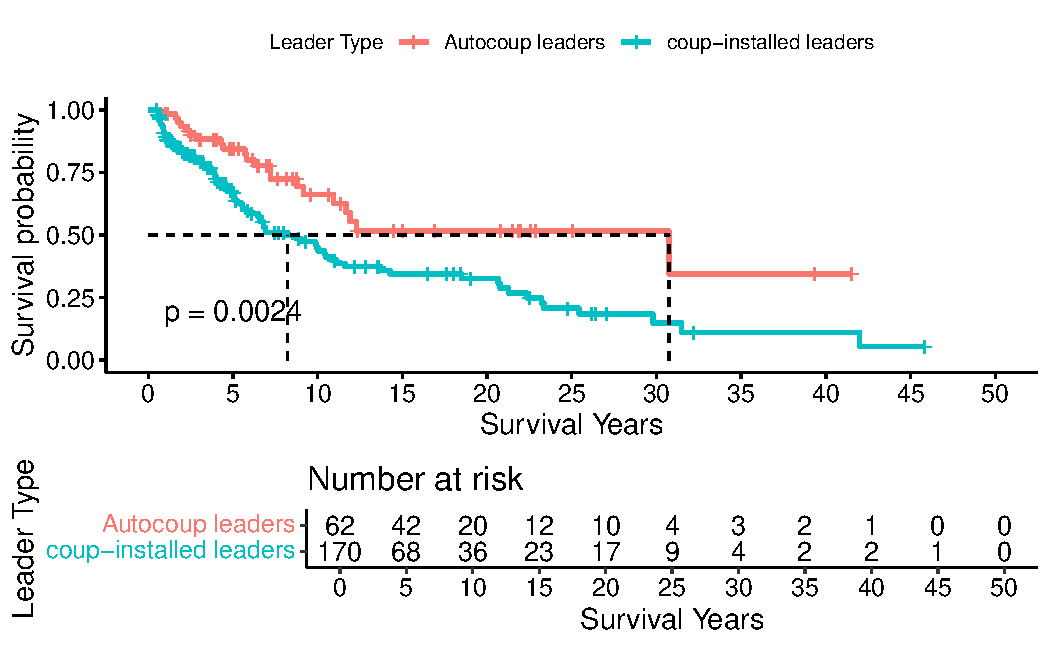
\includegraphics[keepaspectratio]{_coups_and_autocoups_correction_files/figure-pdf/fig-logrank-1.pdf}}

}

\caption{\label{fig-logrank}Survival curves of autocoup and
coup-installed leaders}

\end{figure}%

A preliminary log-rank test in survival analysis, as illustrated in
Figure~\ref{fig-logrank}, demonstrates a statistically significant
difference between the tenures of autocoup and coup-installed leaders.
The survival curve for autocoup leaders consistently exceeds that of
coup-installed leaders, indicating longer survival times and a reduced
risk of ouster for autocoup leaders.

This study posits that the method of accession significantly influences
leadership longevity. Coup-installed leaders likely confront greater
challenges to their rule, resulting in shorter average tenures compared
to autocoup leaders. The analysis, employing Cox proportional hazards
and time-dependent Cox models, supports this hypothesis, demonstrating
that autocoup leaders generally experience longer tenures than
coup-installed leaders.

This research offers two primary contributions to the field. First, it
highlights an understudied factor in leadership survival analysis: the
impact of the method of accession to power. The findings suggest that
leader survival is influenced not only by ruling strategies but also by
the initial method of acquiring power. Second, by employing survival
models, this study provides empirical evidence of the significant
difference in tenure duration between autocoup and coup-installed
leaders. This insight may explain the increasing prevalence of tenure
extensions through autocoups since 2000, as more incumbents observe and
potentially emulate successful precedents.

The remainder of this chapter is structured as follows: Section 2
provides a comprehensive literature review on political survival,
establishing the context for this research. Section 3 explores the
factors influencing the survival of coup and autocoup leaders. Section 4
outlines the methodology and data used, including the application of
survival models to analyze the determinants of leadership longevity.
Section 5 presents the analysis findings and a detailed discussion of
the results. Finally, Section 6 concludes by synthesizing key takeaways
and exploring their broader implications for political stability and
democratic processes.

\section{Literature review}\label{literature-review}

The longevity of political leaders, which varies widely across different
regimes, countries, and historical periods, has been a longstanding
focus of research in political science. This field can be divided into
two interconnected areas: regime survival and individual leader
survival, which are distinct but related concepts. Regime survival
focuses on the endurance of political systems, such as monarchies,
political parties, or specific ideological structures, while leader
survival concerns the duration of individual leaders' time in office.

Political survival patterns vary widely across different systems.
Parliamentary democracies (e.g., Japan, United Kingdom) often experience
prolonged periods of party dominance coupled with frequent leadership
changes. Similarly, communist regimes (e.g., China) typically
demonstrate enduring party rule with more frequent leadership
transitions. Presidential systems (e.g., United States) and many
military regimes tend to exhibit more frequent changes in both ruling
party or junta and leader.

The existing literature on leader survival is extensive and
multifaceted. Some studies explore specific mechanisms influencing
leadership longevity within particular regimes, such as democracies
(\citeproc{ref-svolik2014}{Svolik 2014}) or autocracies
(\citeproc{ref-davenport2021}{Davenport, RezaeeDaryakenari, and Wood
2021}). Others aim to develop more generalizable theoretical frameworks
explaining leader survival across different political systems
(\citeproc{ref-buenodemesquita2003}{Bueno de Mesquita et al. 2003}).
While a universal theory remains an aspirational goal, the complexities
of leadership survival across diverse regime types present significant
challenges.

Power transition mechanisms vary substantially across different types of
regimes, particularly between democracies and autocracies. Autocratic
systems often feature closed leadership selection processes, restricted
to a narrow pool of individuals. While some autocracies may hold
elections, significant barriers to entry for legitimate challengers
typically persist. The opacity of selection processes in autocracies
makes it difficult to assess genuine levels of public support compared
to democracies. Conceptualizing selectorates or winning coalitions, as
proposed by Bueno de Mesquita et al.
(\citeproc{ref-buenodemesquita2003}{2003}), becomes problematic in many
autocratic contexts.

Given these complexities, focusing research on specific regimes or
leader types may be more fruitful. The study of irregular leaders, such
as those who ascend to power through coups or extend their tenures
through autocoups, offers a compelling avenue for research due to the
inherent complexities and uncertainties surrounding their leadership
trajectories.

Two primary perspectives have emerged to explain the dynamics of leader
survival. The first emphasizes objective factors and resources, such as
personal competence (\citeproc{ref-yu2016}{Yu and Jong-A-Pin 2016}),
societal stability (\citeproc{ref-arriola2009}{Arriola 2009}), economic
development (\citeproc{ref-palmer1999}{Palmer and Whitten 1999};
\citeproc{ref-williams2011}{Williams 2011}), natural resource endowments
(\citeproc{ref-smith2004}{Smith 2004};
\citeproc{ref-quirozflores2012}{Quiroz Flores and Smith 2012};
\citeproc{ref-wright2013}{Wright, Frantz, and Geddes 2013}), and
external support (\citeproc{ref-licht2009}{Licht 2009};
\citeproc{ref-wright2008}{Wright 2008}; \citeproc{ref-thyne2017}{C.
Thyne et al. 2017}). The second focuses on subjective factors and
strategies, including political policies, responses to opposition, and
tactics for consolidating power (\citeproc{ref-gandhi2007}{Gandhi and
Przeworski 2007}; \citeproc{ref-morrison2009}{Morrison 2009};
\citeproc{ref-escribuxe0-folch2013}{Escribà-Folch 2013};
\citeproc{ref-davenport2021}{Davenport, RezaeeDaryakenari, and Wood
2021}).

Coups, a significant aspect of irregular leadership transitions, have
received considerable scholarly attention. Research has examined coup
prevention strategies (\citeproc{ref-powell2017}{J. Powell 2017};
\citeproc{ref-sudduth2017}{Sudduth 2017}; \citeproc{ref-debruin2020}{De
Bruin 2020}). Studies have explored the impact of coups on leadership
and the subsequent actions of coup leaders Easton and Siverson
(\citeproc{ref-easton2018}{2018}).

However, a significant gap remains in the literature regarding the
comparison of leadership survival between coup-installed and autocoup
leaders. This study aims to address this gap by investigating and
comparing the duration of leadership survival for these two leader
types.

By focusing on the comparison between coup-installed and autocoup
leaders, this study seeks to contribute to a more nuanced understanding
of political survival in irregular leadership transitions. This approach
may offer valuable insights into the complex dynamics of leader
longevity across different political contexts.

\section{Survival dynamics of autocoup and coup-installed
leaders}\label{survival-dynamics-of-autocoup-and-coup-installed-leaders}

Studying leadership survival in political systems is challenging due to
the opacity and diverse mechanisms of power transitions. These
challenges, however, underscore the significance of this research, as it
illuminates understudied dynamics in political leadership. Although the
survival of political leaders is complex and varied, some patterns do
emerge. Leaders of similar types often exhibit similar characteristics,
allowing for meaningful analysis.

\subsection{Key definitions and scope}\label{key-definitions-and-scope}

Before delving into the comparison, it is essential to clarify several
key terminologies:

\begin{itemize}
\item
  \textbf{Coup and autocoup}: These terms are defined consistently with
  previous chapters to ensure clarity and consistency throughout the
  study.
\item
  \textbf{Tenure length threshold}: To ensure meaningful analysis, this
  study focuses on leaders with substantial periods in power, applying a
  six-month threshold to both autocoup and coup-installed leaders. This
  criterion filters out ephemeral leadership episodes, allowing for a
  more robust examination of survival dynamics.
\item
  \textbf{Autocoup leader}: An incumbent leader who successfully employs
  illegitimate or unconstitutional means to extend their tenure in
  power. This definition encompasses various methods of power
  consolidation that circumvent established democratic processes or
  constitutional limits.
\item
  \textbf{Coup-installed leader}: The individual who assumes power after
  a successful coup, regardless of their role in the coup itself. This
  broad definition allows for the inclusion of both coup instigators and
  those selected to lead post-coup, providing a comprehensive view of
  leadership dynamics following forceful regime change.
\end{itemize}

This study focuses on comparing the post-autocoup tenure of autocoup
leaders with the post-coup tenure of coup-installed leaders. This
comparative approach is motivated by the relevance and similarity of
these leader types in terms of illegitimacy, uncertainty, and
instability. By examining these parallel yet distinct paths to power, we
can gain insights into the factors that influence leadership longevity
in irregular leadership transitions.

\subsection{Challenges in power
consolidation}\label{challenges-in-power-consolidation}

Both autocoup and coup-installed leaders confront distinct challenges in
consolidating their power, primarily stemming from the varying intensity
of issues related to illegitimacy, uncertainty, and instability. This
disparity creates an uneven playing field in terms of power dynamics,
placing coup-installed leaders at a significant disadvantage.
Table~\ref{tbl-leaders} provides a comparative overview of the main
features of autocoup and coup-installed leaders, highlighting these key
differences.

\blandscape

\begin{table}

\caption{\label{tbl-leaders}Main features of autocoup and coup-installed
leaders}

\centering{

\fontsize{12.0pt}{14.4pt}\selectfont
\begin{tabular*}{1\linewidth}{@{\extracolsep{\fill}}>{\raggedright\arraybackslash}p{\dimexpr 112.50pt -2\tabcolsep-1.5\arrayrulewidth}>{\raggedright\arraybackslash}p{\dimexpr 225.00pt -2\tabcolsep-1.5\arrayrulewidth}>{\raggedright\arraybackslash}p{\dimexpr 225.00pt -2\tabcolsep-1.5\arrayrulewidth}}
\toprule
Feature & Autocoup Leader & Coup Entry Leader \\ 
\midrule\addlinespace[2.5pt]
Illegitimacy & Normally attained through
lawful procedures, but
lacking consensus
legitimacy & Blatantly illegal \\ 
Uncertainty & Initially with some certainty, but decreases as the leader's age grows or health worsens & Significant uncertainty initially \\ 
Instability & Relatively stable & Unstable except when a strongman emerges or constitutional institutions are established \\ 
Balance of Power & Generally in a better position of power & Initially unclear and challenging to establish a balance \\ 
\bottomrule
\end{tabular*}

}

\end{table}%

\elandscape

\subsubsection*{Illegitimacy}\label{illegitimacy}
\addcontentsline{toc}{subsubsection}{Illegitimacy}

While both types of leaders suffer from a legitimacy deficit, the nature
and perception of this deficit differ significantly:

\begin{itemize}
\item
  \textbf{Coup-installed leaders}: Their illegitimacy is blatant and
  unambiguous, stemming from the overt and often violent seizure of
  power. This overt act undermines pre-existing norms and institutions,
  generating immediate domestic and international condemnation.
\item
  \textbf{Autocoup leaders}: In contrast, autocoup leaders employ a more
  subtle and deceptive strategy, manipulating legal processes and
  institutions to create a façade of democratic legitimacy. This veneer
  of legality, while often thin, can provide a degree of cover and buy
  time for consolidating power.
\end{itemize}

\subsubsection*{Uncertainty}\label{uncertainty}
\addcontentsline{toc}{subsubsection}{Uncertainty}

The irregular paths to power for both types of leaders create
uncertainty about the longevity of their rule and the mechanisms of
their eventual departure. However, the levels and sources of this
uncertainty differ significantly.

\begin{itemize}
\item
  \textbf{Coup-installed leaders:} These leaders face a trifecta of
  uncertainties. First, the immediate aftermath of a coup often involves
  a struggle for power within the junta or ruling coalition, creating
  ambiguity about who will ultimately consolidate control. Second, the
  tenure of coup-installed leaders is inherently precarious, subject to
  internal rivalries, popular uprisings, or counter-coups. Third, the
  lack of established succession mechanisms further amplifies
  uncertainty, making it difficult to predict the transfer of power and
  potentially triggering future instability.
\item
  \textbf{Autocoup leaders:} While not immune to uncertainty, autocoup
  leaders generally present a clearer picture. The question of who will
  rule post-autocoup is largely settled, as the incumbent retains power.
  Furthermore, many autocoup leaders openly aspire to extend their rule
  indefinitely or incrementally, attempting to establish a sense of
  permanence. This perceived stability, whether real or manufactured,
  can contribute to a more predictable political environment, at least
  in the short term.
\end{itemize}

\subsubsection*{Instability}\label{instability}
\addcontentsline{toc}{subsubsection}{Instability}

The awareness of shaky legitimacy and persistent uncertainty inevitably
breeds insecurity and a sense of crisis, forcing both autocoup and
coup-installed leaders to prioritize stabilization measures. However,
the nature and intensity of these challenges differ:

\begin{itemize}
\item
  \textbf{Coup-installed leaders:} These leaders face the daunting task
  of rapidly reshaping power dynamics, often resorting to purges and
  crackdowns to eliminate potential adversaries and consolidate control.
  This process of dismantling existing structures and building new ones
  generates significant instability, potentially alienating former
  allies and triggering resistance from various segments of society. The
  need to appease powerful actors both domestically and internationally
  further limits their options, forcing them into compromises that can
  undermine their authority and long-term stability.
\item
  \textbf{Autocoup leaders:} In contrast, autocoup leaders often benefit
  from a degree of continuity in regime personnel and institutions. This
  relative stability allows them to implement changes gradually,
  minimizing disruptions and mitigating potential backlash. While they
  may still face opposition, they are less likely to confront immediate
  and existential threats to their rule, providing them with more time
  and leverage to consolidate power.
\end{itemize}

By understanding these contrasting challenges, we can better appreciate
the relative advantages and disadvantages faced by autocoup and
coup-installed leaders. This comparative perspective provides a nuanced
framework for analyzing the strategies these leaders employ to
consolidate power and navigate the perilous terrain of irregular
leadership transitions.

\subsection{Empirical evidence and
hypothesis}\label{empirical-evidence-and-hypothesis}

Empirical evidence substantiates the disadvantage faced by
coup-installed leaders, revealing a complex interplay between historical
precedent, power consolidation challenges, and leadership longevity.
This section presents key data points and introduces the central
hypothesis guiding this study.

Data analysis shows a significant correlation between the frequency of
coup attempts in a country and the likelihood of future coups. Notably,
over a third of coups have occurred in the top ten countries with the
most attempts since 1950 (As shown in \textbf{?@tbl-coups}). This
pattern suggests a self-reinforcing cycle of political instability,
where each successful coup increases the probability of subsequent
attempts, creating an environment of persistent uncertainty for
coup-installed leaders.

The disparity in leadership longevity between autocoup and
coup-installed leaders is starkly illustrated by survival data. As
depicted in Figure~\ref{fig-logrank}, the average survival period
following an autocoup is approximately five years longer than that of
coup-installed leaders. This substantial difference in tenure length
underscores the divergent challenges faced by these two types of leaders
in maintaining their grip on power.

The distinct challenges faced by autocoup leaders and coup-installed
leaders in consolidating power create a self-perpetuating cycle that
significantly influences their tenure length:

\begin{itemize}
\item
  Coup-installed leaders: Face greater legitimacy challenges and
  internal instability; Struggle to attract and retain strong support;
  More vulnerable to internal and external challenges; Shorter average
  tenures reinforce perception of instability.
\item
  Autocoup leaders: Often benefit from a veneer of legitimacy and a
  stronger initial position; Better able to consolidate power and
  attract supporters; Face less immediate threat of overthrow; Longer
  average tenures contribute to perception of stability.
\end{itemize}

This cycle suggests that the initial method of power acquisition or
extension has far-reaching consequences for a leader's ability to
maintain their position over time.

Based on these observations and the theoretical framework outlined
earlier, I propose the following hypothesis:

\textbf{\emph{H4-1: Political leaders who successfully extend their
tenure through autocoups are more likely to survive longer extended
tenure compared to coup-installed leaders.}}

This hypothesis encapsulates the expected outcome of the divergent
challenges and advantages faced by autocoup and coup-installed leaders.
By testing this hypothesis, I aim to quantify the impact of the method
of power acquisition or extension on leadership longevity, contributing
to a more nuanced understanding of political survival in contexts of
irregular transitions.

\section{Research design}\label{research-design-1}

This section employs survival analysis to test the hypothesis that
autocoup leaders have longer survival times in office compared to
coup-installed leaders. This study uses Cox models to analyze the
survival tenures of autocoup and coup-installed leaders, controlling for
various factors that may affect their time in office.

\subsection{Methodology: Survival
analysis}\label{methodology-survival-analysis}

Two Cox models will be employed to analyze the survival tenures of
coup-installed and autocoup leaders:

\begin{itemize}
\item
  \textbf{Cox proportional hazards (PH) model}: This model uses only the
  variables present at the entry year, without considering changes over
  time.
\item
  \textbf{Time-dependent Cox model}: This model accounts for variations
  in time-dependent control variables such as economic performance and
  political stability.
\end{itemize}

The Cox model is preferred over the Kaplan-Meier model because it
enables the estimation of the impact of multiple factors. Although it
does not directly estimate the duration of tenure, it assesses the
hazard rate associated with being ousted from power. This approach
captures different facets of the same phenomenon: as a leader's
cumulative hazard of being ousted increases, their probability of
survival in office decreases.

\subsection{Data and variables}\label{data-and-variables-1}

The dependent variables include survival time and end point status:

\begin{itemize}
\item
  \textbf{Survival time:} Survival time refers to the duration of a
  leader's tenure, measured in days. For coup-installed leaders, the
  survival time begins on the day they assume power through a coup. For
  autocoup leaders, the survival time starts on the expiration date of
  their original legitimate term. For example, Russia's president
  Vladimir Putin assumed power in 2000 and, after serving two terms,
  stepped down in 2008. However, he remained in a powerful position as
  the prime minister and hand-picked Dmitry Medvedev to succeed him as
  president, while continuing to control the power behind the scenes. In
  this case, Putin's survival time begins in 2008, marking the start of
  his post-autocoup tenure. The survival time concludes on the day the
  leader finally exits office, applicable to both coup-installed and
  autocoup leaders.
\item
  \textbf{End point status:} This variable indicates the manner in which
  the leader's tenure concluded, categorized as follows:

  \textbf{0 = Censored:} This status is assigned to leaders who leave
  office through regular means other than being ousted. This includes
  leaders transferring power to their designated successors, leaving
  office as their terms expire, losing in general elections, voluntarily
  leaving office due to health issues, or dying of natural causes.

  \textbf{1 = Ousted:} This status is assigned to leaders who are forced
  to leave office. This includes leaders resigning under pressure, being
  ousted by coups or other forces, or being assassinated.
\end{itemize}

The key independent variable is the leader type, which categorizes
leaders into two distinct groups:

\begin{itemize}
\tightlist
\item
  \textbf{Group A = Autocoup leader}: Leaders who extend their tenure
  through autocoups.
\item
  \textbf{Group B = Coup-installed leader}: Leaders who assume power
  through coups.
\end{itemize}

This variable is the primary independent variable of interest, serving
as the basis for comparing the survival time between these two types of
leaders.

The data for both dependent and independent variables are sourced from
the autocoup dataset introduced in this study, Archigos, and PLAD.

Control variables include economic performance, political stability,
population size, and the leader's age, which are consistent with the
autocoup analysis in Chapter~\ref{sec-chapter3}.

\section{Results and discussion}\label{results-and-discussion}

\subsection{Model results}\label{model-results}

Using the \textbf{\emph{surviavl}} package in R
(\citeproc{ref-survival}{Therneau 2024}), I present the regression
results for both the Cox Proportional Hazards model (Cox PH) and the
time-dependent Cox model in Table~\ref{tbl-cox}.

\begin{table}

\caption{\label{tbl-cox}Cox models for survival time of different types
of leaders}

\centering{

\fontsize{12.0pt}{14.4pt}\selectfont
\begin{tabular*}{\linewidth}{@{\extracolsep{\fill}}lcccccccc}
\toprule
 & \multicolumn{4}{c}{\textbf{Cox PH Model}} & \multicolumn{4}{c}{\textbf{Time-dependent Cox Model}} \\ 
\cmidrule(lr){2-5} \cmidrule(lr){6-9}
\textbf{Characteristic} & \textbf{N} & \textbf{Event N} & \textbf{HR}\textsuperscript{\textit{1,2}} & \textbf{SE}\textsuperscript{\textit{2}} & \textbf{N} & \textbf{Event N} & \textbf{HR}\textsuperscript{\textit{1,2}} & \textbf{SE}\textsuperscript{\textit{2}} \\ 
\midrule\addlinespace[2.5pt]
{\bfseries Leader Type} &  &  &  &  &  &  &  &  \\ 
    Autocoup leaders & 67 & 30 & 1.00 & — & 50 & 25 & 1.00 & — \\ 
    Coup-installed leaders & 163 & 163 & 8.39*** & 0.240 & 167 & 167 & 1.87*** & 0.269 \\ 
{\bfseries GDP Growth Trend} & 230 & 193 & 0.20 & 1.18 & 217 & 192 & 1.02 & 1.26 \\ 
{\bfseries GDP per capita} & 230 & 193 & 0.99 & 0.011 & 217 & 192 & 0.93*** & 0.036 \\ 
{\bfseries Population: log} & 230 & 193 & 1.13* & 0.064 & 217 & 192 & 1.12** & 0.065 \\ 
{\bfseries Polity 5} & 230 & 193 & 0.99 & 0.013 & 217 & 192 & 0.96*** & 0.015 \\ 
{\bfseries Political stability} & 230 & 193 & 1.05 & 0.042 & 217 & 192 & 1.12*** & 0.048 \\ 
{\bfseries Age} & 230 & 193 & 1.03*** & 0.008 & 217 & 192 & 1.02*** & 0.007 \\ 
\bottomrule
\end{tabular*}
\begin{minipage}{\linewidth}
\textsuperscript{\textit{1}}*p\textless{}0.1; **p\textless{}0.05; ***p\textless{}0.01\\
\textsuperscript{\textit{2}}HR = Hazard Ratio, SE = Standard Error\\
\end{minipage}

}

\end{table}%

Both models showed a statistically significant relationship between
leadership type and the hazard of removal from power. Since
time-dependent Cox model use the control variables which change over
time, I interpret the main findings based on time-dependent model.

Coup-installed leaders were found to have a hazard ratio of 2.23 in the
time-dependent model compared to autocoup leaders (reference group),
assuming all other variables in the model are held constant. This
suggests that coup-installed leaders face a significantly greater risk
of removal from power compared to autocoup leaders. At any given time
during their tenure, coup-installed leaders are 2.23 times more likely
to be ousted from power compared to autocoup leaders, all else being
equal in the model.

The control variables perform differently in the two models. Economic
level (GDP per capita) exhibits statistically significant effects in
both models. In the time-dependent model, the hazard ratio of 0.95
indicates that for each unit increase in GDP per capita (measured in
units of \$10,000), the hazard (or risk) of being ousted at any given
time is reduced by 5\%, assuming all other variables in the model are
held constant.

GDP growth trend demonstrates a more substantial effect in reducing the
risk of coups. Specifically, a 1 percentage point higher economic growth
trend is associated with an 80\% reduction in the risk of being ousted,
although this effect is only statistically significant at the 10\%
level. This suggests a possible trend where positive economic
performance might mitigate the risk of removal from power, but the
evidence is not robust enough to confirm this conclusively.

Political stability, as measured by the violence index, shows that a
1-point increase in the index correlates with an 11\% higher risk of
being ousted. However, this effect is also only statistically
significant at the 10\% level, indicating a weaker but potentially
important relationship between increased violence and the risk of
removal from office.

\subsection{Discussion}\label{discussion}

\begin{figure}

\begin{minipage}{0.50\linewidth}

\centering{

\pandocbounded{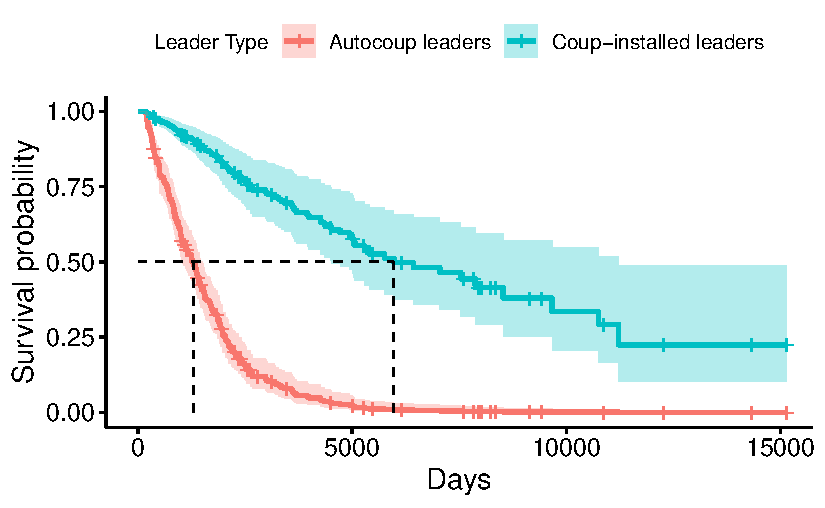
\includegraphics[keepaspectratio]{_coups_and_autocoups_correction_files/figure-pdf/fig-coxSurv-1.pdf}}

}

\subcaption{\label{fig-coxSurv-1}Cox PH Model}

\end{minipage}%
%
\begin{minipage}{0.50\linewidth}

\centering{

\pandocbounded{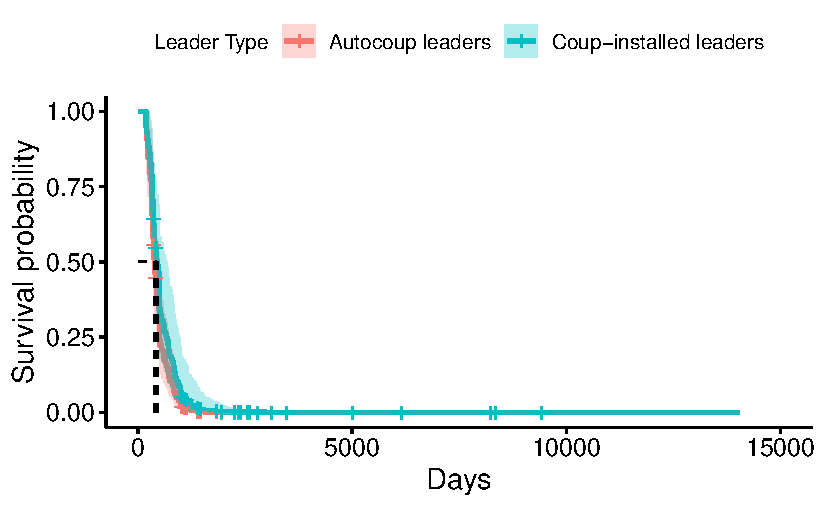
\includegraphics[keepaspectratio]{_coups_and_autocoups_correction_files/figure-pdf/fig-coxSurv-2.pdf}}

}

\subcaption{\label{fig-coxSurv-2}Time-dependent Cox Model}

\end{minipage}%

\caption{\label{fig-coxSurv}Survival curves for Cox Model}

\end{figure}%

The survival curves in Figure~\ref{fig-coxSurv} displays the survival
rates for both types of leaders, highlighting the differences in their
survival curves. Both the Cox PH model and the time-dependent Cox model
yield similar results. Notably, the survival curve for coup-installed
leaders has a significantly lower trajectory than that of autocoup
leaders. The steeper drop at the early stage for coup-installed leaders
indicates they are more likely to be ousted shortly after assuming
power. Additionally, the survival curve for coup-installed leaders
crosses the median survival line much earlier (about 3,000 days) than
that of autocoup leaders (about 8,500 days). This disparity suggests
that autocoup leaders tend to remain in power for longer durations than
their coup-installed counterparts.

\begin{figure}

\begin{minipage}{0.50\linewidth}

\centering{

\pandocbounded{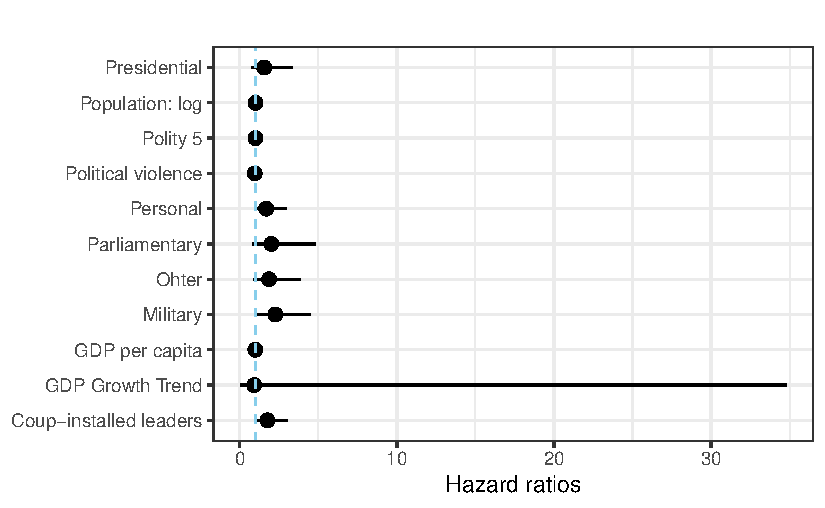
\includegraphics[keepaspectratio]{_coups_and_autocoups_correction_files/figure-pdf/fig-coxHR-1.pdf}}

}

\subcaption{\label{fig-coxHR-1}Cox PH Model}

\end{minipage}%
%
\begin{minipage}{0.50\linewidth}

\centering{

\pandocbounded{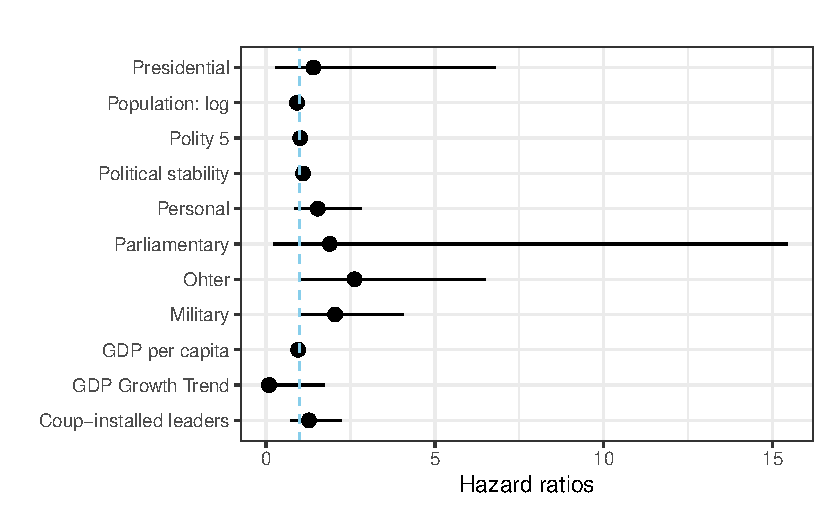
\includegraphics[keepaspectratio]{_coups_and_autocoups_correction_files/figure-pdf/fig-coxHR-2.pdf}}

}

\subcaption{\label{fig-coxHR-2}Time-dependent Cox Model}

\end{minipage}%

\caption{\label{fig-coxHR}Hazard ratios and 95\% CIs for Leader Ousting}

\end{figure}%

Figure~\ref{fig-coxHR} displays the hazard ratios and corresponding 95\%
confidence intervals for the variables incorporated in the Cox model.
Both the Cox Proportional Hazards (PH) model and the time-dependent
model produce similar plots, reinforcing the robustness of the findings.
Key points to note include:

\begin{itemize}
\item
  The closer the hazard ratio (represented by the dots) is to 1, the
  less impact the variable has on the risk of being ousted. A hazard
  ratio of 1 indicates no effect.
\item
  The whiskers extending from the dots represent the 95\% confidence
  intervals. If these whiskers cross the vertical blue line at 1, it
  indicates that the variable is not statistically significant at the
  5\% level.
\item
  The hazard ratio for coup-installed leaders is significantly greater
  than 1 and statistically significant at the 5\% level. This indicates
  that coup-installed leaders face a substantially higher risk of being
  ousted compared to autocoup leaders.
\item
  Most other variables have hazard ratios close to 1, suggesting that a
  one-unit increase in these variables does not significantly affect the
  risk of being ousted.
\item
  Although the hazard ratio for GDP growth trend is considerably less
  than 1 in the time-dependent model, indicating a potential protective
  effect, it is not statistically significant at the 5\% level. However,
  it is statistically significant at the 10\% level, suggesting that
  better economic performance may help to consolidate the rule of the
  incumbents to some extent, albeit the evidence is not as strong.
\end{itemize}

\subsection{Assessing the proportional hazards
assumption}\label{assessing-the-proportional-hazards-assumption}

Assessing the proportional hazards assumption is crucial for the
validity of the Cox model results. To evaluate this, we used the
chi-square test based on Schoenfeld residuals to determine whether the
covariate effects remain constant (proportional) over time. Although the
Cox PH model violates the proportional hazards assumption, our primary
analysis relies on the time-dependent Cox model, which does not show
strong evidence of violating the proportional hazards assumption for any
covariate. The global p-value of 0.416 is much greater than the 5\%
significance level, indicating that the proportional hazards assumption
is reasonably met for the time-dependent Cox model.

\section{Summary}\label{summary-2}

This chapter explores the survival durations of political leaders who
come to power through unconventional means, specifically focusing on
coups and autocoups. Based on the hypothesis that the mode of accession
affects leader tenure, I use survival analysis techniques, including the
Cox proportional hazards model and a time-dependent Cox model, to
investigate this phenomenon. The findings suggest that autocoup leaders
tend to have longer tenures than coup-installed leaders.

Empirical analysis reveals a significant disparity in tenure length:
leaders who assume power via autocoup remain in office for an average of
11 years, compared to just 5.6 years for those installed by coups.
Moreover, the time-dependent Cox model indicates that coup-installed
leaders are 2.23 times more likely to be ousted from power at any given
time compared to their autocoup counterparts, all other factors being
equal. These findings underscore the importance of understanding the
autocoup as a mechanism through which leaders extend their rule by
manipulating legal frameworks and weakening institutional constraints.

The implications of these findings are profound. The relative ease and
potential rewards of an autocoup could incentivize more leaders to
resort to this method of power retention, particularly in fragile
democracies or transitioning regimes. Consequently, democratic
backsliding may become more prevalent, as autocoups erode democratic
institutions and undermine constitutional norms.

This study contributes significantly to the literature on political
leadership survival by showing that the mode of accession has a
substantial impact on leader tenure, an aspect that has received limited
attention in previous research. Methodologically, this work advances the
field by applying robust survival analysis techniques, including both
Cox models, to provide a nuanced understanding of the dynamics that
influence leadership stability.

However, the study is not without limitations. The analysis relies on an
autocoup dataset that was collected and coded by the author, a
relatively novel concept in the academic sphere. As the understanding
and recognition of ``autocoup'' as a term continue to evolve, future
research should refine and expand the dataset. Incorporating additional
cases and cross-referencing with other forms of irregular leadership
transitions would contribute to a more comprehensive view of political
survival under such conditions.

In conclusion, this chapter highlights the need for more refined
approaches to studying political tenure and irregular power retention.
By offering valuable insights into the dynamics of political stability
and the risks associated with non-democratic leadership transitions,
this research emphasizes the importance of continued investigation into
the complex relationships between power, legitimacy, and survival in
political leadership.

\chapter{Coups, Autocoups, and
Democracy}\label{coups-autocoups-and-democracy}

\section*{Abstract}\label{abstract-4}
\addcontentsline{toc}{section}{Abstract}

This chapter explores the impact of autocoups on political institutions,
drawing comparisons with traditional coups through an analysis of
changes in Polity scores. I contend that, first, incumbent leaders
frequently consolidate power by undermining established institutions in
anticipation of an autocoup, resulting in a decline in Polity scores
even prior to the event. Second, unlike coups, which produce mixed
outcomes regarding democratization, autocoups almost invariably lead to
democratic backsliding or authoritarian entrenchment, as they are
specifically designed to dismantle institutional checks, enabling
leaders to maintain power for significantly longer periods than those
installed via coups.

Employing a country-fixed effects model and utilizing datasets on both
autocoups and coups, this study reveals that Polity scores decline both
preceding and following an autocoup, while coups tend to trigger an
immediate decrease that may allow for some degree of democratic recovery
over time. These findings underscore the divergent political
trajectories associated with coups and autocoups. This research not only
addresses a critical gap in the empirical analysis of autocoups but also
significantly raises awareness within academic and policy-making circles
regarding their potential adverse effects, including democratic
backsliding and further authoritarian deterioration.

\section{Introduction}\label{introduction-4}

In the preceding chapters, I clarified the definition of an autocoup,
introduced a novel dataset on autocoups, conducted empirical analyses on
the determinants of autocoup attempts, and compared the post-event
survival times of leaders established through coups versus autocoup
leaders. A natural follow-up question emerges: What are the broader
impacts of autocoups? Specifically, from a political science
perspective, how do autocoups affect the process of democratization?

As previously noted, due to the absence of a widely recognized dataset
on autocoups, most existing discussions on their impact have relied on
case studies (\citeproc{ref-baturo}{Baturo and Elgie, n.d.};
\citeproc{ref-baturo2022}{Baturo and Tolstrup 2022}). To move beyond
case-specific analyses and adopt a more systematic and comparative
approach, this chapter aims to pioneer empirical research on the
democratic consequences of autocoups. The first objective of this
chapter, therefore, is to examine whether autocoups reinforce
authoritarianism, promote democratization, or have no significant effect
on political regimes.

Given the conceptual and empirical connections between coups and
autocoups, another key objective is to compare their respective effects
on democratization. While both events disrupt existing political orders,
their immediate and long-term consequences may vary significantly.
Understanding these distinctions is essential for evaluating their
broader implications.

To address these questions, this study leverages data from a widely
recognized coup dataset alongside a newly compiled dataset on autocoups.
Employing a fixed-effects model, it evaluates their effects on
democracy, as measured by the Polity Index. The findings reveal that
both coups and autocoups lead to an immediate decline in democratic
levels. However, coups have a more pronounced negative short-term
impact. Notably, three years after these events, democracies affected by
coups tend to show significant recovery, whereas those experiencing
autocoups exhibit no meaningful improvement.

This study offers two significant contributions to the field of
political science. First, it provides the inaugural empirical analysis
of the impact of autocoups on democratization, effectively addressing a
critical gap in the existing literature. Second, by directly comparing
the effects of coups and autocoups, this research highlights autocoups
as a distinct phenomenon that demands increased scholarly inquiry and
policy focus.

The remainder of this chapter is structured as follows: Section 2
analyzes the impact of autocoups on democratization, by comparing the
effects with traditional coups. Section 3 outlines the research design,
methodology, and variables used in this study. Section 4 presents and
interprets the empirical findings, followed by a discussion of their
implications. Finally, Section 5 concludes by summarizing the key
results and exploring their significance for understanding and
mitigating the occurrence of autocoups.

\section{Impact of autocoups on political
change}\label{impact-of-autocoups-on-political-change}

According to the definition in \textbf{?@sec-definition}, an autocoup
refers to an incumbent leader extending their tenure in power beyond the
originally mandated limits, whether through legal or illegal means.
While the leader may assume a different title or position, the
individual in power remains unchanged. Therefore, unlike traditional
coups, an autocoup does not result in real leadership turnover, elite
restructuring, or regime change. In other words, the fundamental ruling
structure remains intact.

This distinction has important implications. Since regime change rarely
occurs following an autocoup, its impact on politics cannot be assessed
using conventional methods. Typically, studies on coups and
democratization measure their effects by estimating the probability of
regime transition---either from autocracy to democracy or vice
versa---as seen in previous research on coup outcomes
(\citeproc{ref-thyne2014}{C. L. Thyne and Powell 2014};
\citeproc{ref-derpanopoulos2016}{Derpanopoulos et al. 2016};
\citeproc{ref-miller2016}{Miller 2016}). However, this approach is not
suitable for autocoups, as they do not directly trigger regime
transfers.

Although autocoups rarely lead to formal regime change, this does not
mean they have no impact on political dynamics. In fact, they inevitably
shape political trajectories in various ways and, on occasion, can even
lead to significant transformations. Therefore, a more appropriate
method for assessing the political impact of autocoups is to analyze
democratic indices, such as those measured by Polity5
(\citeproc{ref-p1}{Monty G. Marshall and Gurr 2020}). The Polity Score,
ranging from -10 (full autocracy) to +10 (full democracy), captures
gradual shifts in political regime characteristics rather than abrupt
transitions. Thus, even if an autocoup does not result in a formal
regime change, subtle shifts in political openness and institutional
constraints can still be assessed by examining variations in Polity
scores before and after the event. This approach has also been employed
in previous studies (\citeproc{ref-dahl2023}{Dahl and Gleditsch 2023}).

Although autocoups may not lead to significant regime change, their
impact on democratization should not be overlooked. However, their
influence differs from that of traditional coups in at least two key
ways.

\subsection{\texorpdfstring{\textbf{The pre-emptive effects of autocoups
on political
dynamics}}{The pre-emptive effects of autocoups on political dynamics}}\label{the-pre-emptive-effects-of-autocoups-on-political-dynamics}

First and foremost, unlike coups, which are marked by clear, decisive
events---such as the removal of a leader---autocoups typically unfold
gradually, through incremental steps rather than a singular, dramatic
event. Incumbent leaders seeking to extend their tenure often lay the
groundwork well in advance before executing their final move to remain
in power. To reduce resistance and opposition, they engage in extensive
preparation, which may include purging officials, suppressing political
opposition, cracking down on dissent and protests, and restricting press
freedom. Without such measures, an autocoup might face strong internal
resistance, and in the worst case, provoke a backlash that not only
derails the leader's attempt to extend their rule but also results in
their immediate removal from office.

However, once an incumbent successfully secures an extension of their
rule, continued repression is not always necessary. On the contrary,
some leaders relax political pressure to ease internal dissent and
mitigate opposition from external actors. This adaptive approach helps
maintain stability after the autocoup is complete.

As a result, the primary impact of autocoups on political change is
often reflected in shifts in political scores before the final stage of
the autocoup is enacted. Once the process is completed, further shifts
may be minimal. In contrast, coup plotters, unlike incumbents, lack the
ability to influence political institutions beforehand, meaning their
impact on politics is often felt in the aftermath rather than before the
event.

This distinction is evident in empirical cases of autocoups.

One of the most frequently cited examples of an autocoup is Peru's 1992
case, in which President Alberto Fujimori dissolved Congress,
temporarily suspended the 1979 Constitution, and ruled by decree until
November of that year, when a \emph{Democratic Constituent Congress} was
elected to draft a new constitution (\citeproc{ref-cameron1998}{Maxwell
A. Cameron 1998b}). However, these moves did not immediately grant
Fujimori a longer tenure in office.

Under the 1979 Peruvian Constitution, immediate presidential re-election
was prohibited. To bypass this restriction, Fujimori initiated a
constitutional overhaul, leading to the adoption of a new constitution
in 1993, which permitted re-election. Consequently, he secured a second
term in 1995 (\citeproc{ref-baturo2019}{Baturo 2019}).

An analysis of Peru's Polity5 scores during this process reflects these
political changes. Upon taking office in 1990, Peru's Polity score was
8, remaining unchanged in 1991. However, a dramatic shift occurred in
1992, when Fujimori dissolved Congress, causing the Polity score to
plummet from 8 to -4. Interestingly, when he formally extended his rule
by amending the constitution in 1993, the score rebounded slightly to
-1. This -1 score remained unchanged throughout Fujimori's tenure until
2000, indicating a lack of further institutional transformation after
the constitutional amendment.

A similar pattern emerges in Belarus under Alexander Lukashenko. Upon
assuming office as president in 1994, Belarus had a Polity5 score of 8.
However, in 1995, when Lukashenko moved to hold a referendum---defying
opposition in the Supreme Council and threatening to suspend its
activities---the score dropped sharply to 0. Following the 1996
referendum, which extended his term by two additional years, Lukashenko
officially overstayed his tenure. Consequently, the Polity5 score
further declined to -7 in 1996, where it has remained ever since,
despite two additional term extensions (\citeproc{ref-ash2014}{Ash
2014}; \citeproc{ref-baturo}{Baturo and Elgie, n.d.}).

These cases illustrate a broader pattern: the impact of autocoups on
political change is often reflected before the final stage of the
autocoup is enacted, whereas the impact of coups tends to materialize
afterwards, as have been fully discussed by previous studies.

Based on this analysis, I propose the first hypothesis:

\begin{quote}
\emph{H1}: Autocoups primarily shape political change in advance,
whereas coups typically drive political change only after they are
executed.
\end{quote}

\subsection{\texorpdfstring{\textbf{The singular nature of
autocoups}}{The singular nature of autocoups}}\label{the-singular-nature-of-autocoups}

Secondly, in contrast to the ambiguous nature of coups
(\citeproc{ref-dahl2023}{Dahl and Gleditsch 2023}), the impact of
autocoups on political change rarely contributes to democratization.

The influence of coups on democratization has been extensively examined
in existing literature. Some scholars argue that coups---and even the
mere threat of them---can act as catalysts for democratization. One
argument suggests that coups deliver a political ``shock'' that may
create opportunities for liberalization that would not have otherwise
materialized (\citeproc{ref-thyne2014}{C. L. Thyne and Powell 2014}). In
a critical examination, Derpanopoulos et al.
(\citeproc{ref-derpanopoulos2016}{2016}) questioned the role of coups in
promoting democracy, engaging in multiple rounds of debate with Miller
(\citeproc{ref-miller2016}{2016}). More recently, Dahl and Gleditsch
(\citeproc{ref-dahl2023}{2023}) further explored this ongoing
discussion, arguing that both democratic and autocratic transitions are
likely to follow a coup, with popular mobilization playing a decisive
role in shaping post-coup trajectories.

A frequently cited example of a ``pro-democracy coup'' occurred in
February 2010, when Nigerien troops ousted President Mamadou Tandja
after he extended his rule autocratically. The Supreme Council for the
Restoration of Democracy (CSRD) took control, pledging democratic
reforms. Their actions were widely celebrated, with both citizens and
political opposition viewing the coup as an opportunity to restore
democracy. The CSRD fulfilled its commitment by overseeing free and fair
elections in 2011, resulting in Mahamadou Issoufou assuming the
presidency (\citeproc{ref-miller2016}{Miller 2016}).

While the debate on the democratic consequences of coups remains
ongoing, it is evident that their impact is not uniform. In contrast,
autocoups almost never lead to democratic transitions, nor do they even
marginally enhance political freedoms. This stems from the intrinsic
nature of autocoups, which disrupt the established process of political
leadership transition, particularly term limits.

Term limits are constitutional provisions that restrict the maximum
duration a leader can remain in office. They play a crucial role in both
democracies and autocracies by preventing the excessive concentration of
power and ensuring political stability. In democracies, term limits
promote accountability, leadership renewal, and reduce the risks of
corruption and authoritarian entrenchment. In autocracies, when
enforced, they can curb indefinite rule, mitigate succession crises, and
provide rare opportunities for political transitions. However, without
term limits, leaders can entrench themselves in power, undermining
institutions and hindering political progress.

As shown in Table~\ref{tbl-autocoup_method} in Chapter 3, autocoups are
executed through either façade legal mechanisms or blatantly illegal
methods. This includes amending or disregarding term limits, delaying or
cancelling elections, rigging electoral outcomes, or outright refusing
to accept election results. While many autocoups maintain a veneer of
legality, their defining characteristic is the violation of term limits,
which are intended as safeguards against prolonged and unchecked rule.

As previously discussed, before an incumbent leader formally overstays
their term, they often inflict significant damage on political
institutions. Furthermore, to secure their prolonged rule, they are
unlikely to fully restore political freedoms even if they temporarily
ease political repression once they have consolidated power.

Case studies from Peru and Belarus illustrate how autocoups lead to a
decline in Polity scores, reflecting democratic backsliding. However,
most autocoups occur in already autocratic regimes where Polity scores
are low. This aligns with trends observed in coups, which also primarily
occur in autocracies.

For instance, in China's 2018 constitutional amendment, Xi Jinping
abolished presidential term limits, effectively allowing himself to
remain in power indefinitely\footnote{\textbf{BBC News,} ``China's Xi
  Allowed to Remain `President for Life' as Term Limits Removed,''
  \emph{BBC News}, March 11, 2018,
  \url{https://www.bbc.co.uk/news/world-asia-china-43361276}, accessed
  March 14, 2025.}. However, China's Polity score remained unchanged at
-7 before and after the amendment. This pattern is common in autocratic
regimes with Polity scores below -6, as they already lack significant
democratic features, leaving little room for further decline.

While most autocoups occur in low-Polity-score countries, some have
taken place in relatively democratic settings, where the Polity score
remains stable despite term limit extensions. This is particularly
evident in Latin America, where presidents have amended ``no immediate
re-election'' rules to allow for a second consecutive term, but
voluntarily stepped down afterwards. Examples include: Argentina (1993),
Polity score remained at 7; Brazil (1997), Polity score remained at 8,
Colombia (2004), Polity score remained at 7. In these cases, leaders
extended their tenure within a structured political framework without
further dismantling democratic institutions
(\citeproc{ref-baturo2019}{Baturo 2019}).

Across all cases---whether in Peru, Belarus, China, Argentina, Brazil,
or Colombia---there is no instance where a Polity score increased
following an autocoup. In the autocoup dataset which I introduced in
Chapter 3, only four cases---Guinea-Bissau (1988), Burkina Faso (1997),
Congo-Brazzaville (2001), and Lebanon (2004)---saw minor increases in
Polity scores, but the changes were insignificant.

Thus, unlike some coup leaders who justify their actions by claiming to
restore democracy (as seen in Niger's 2010 case), leaders who execute
autocoups lack any democratic justification. If their true intention
were to advance democracy, they would transfer power peacefully rather
than violate term limits.

Based on this analysis, I propose the second hypothesis:

\begin{quote}
\emph{H2}: Autocoups are more likely to entrench autocracy than coups.
\end{quote}

\section{Methodology and variables}\label{methodology-and-variables}

\subsection{Methodology}\label{methodology-1}

As discussed earlier, autocoups are less likely to result in full regime
transitions---either from democracy to autocracy or vice versa.
Therefore, it is inappropriate to assess their effects solely based on
regime transitions or changes that cross a critical threshold. Instead,
this study examines political changes through fluctuations in Polity5
scores.

Unlike coup analysis, which primarily focuses on post-event effects,
this study examines both pre-event and post-event impacts of autocoups.
Specifically, pre-event effects are measured by the change in Polity5
scores three years before the autocoup compared to the year of the
autocoup, expressed as:

\(Polity_t - Polity_{t-3}\)

Post-event effects are measured by the change in Polity5 scores three
years after the autocoup compared to the year of the autocoup, expressed
as:

\(Polity_{t+3} - Polity_t\)

The three-year window is chosen for two key reasons. Pre-event political
changes typically occur incrementally, as incumbents consolidate power
gradually over several years rather than through a single, abrupt
action. Post-event analysis focuses on medium-term effects rather than
short-term shocks, as autocoups rarely trigger immediate regime
transitions and instead reinforce existing political structures.
Short-term fluctuations may be too minor to capture meaningful
institutional change empirically.

To estimate how political institutions change before and after
autocoups, I employ a linear model with country-case fixed effects. For
pre-event effects, I analyze attempted autocoups, since before the
event, no one knows whether the autocoup will succeed or fail.

For post-event effects, I analyze only successful autocoups for three
reasons: The majority of autocoups succeed (87 out of 110 cases); failed
autocoups tend to produce immediate political shocks, rather than
medium- or long-term effects; failed autocoups are often followed by
major disruptive events, such as coups, insurrections, or mass protests,
making it difficult to isolate their impact. For example, in Niger's
case, a failed autocoup in 2009 was followed by a coup in 2010, creating
overlapping political effects. In contrast, successful autocoups provide
a clearer analytical framework, as their effects are less entangled with
other disruptions, allowing for a more systematic assessment of
institutional change.

\subsection{Variables}\label{variables}

This study uses a global sample of all country-year data from 1950 to
2020, applying a linear model to examine the effects of autocoups on
political change. The dependent variable is the change in Polity scores,
while the main independent variable is autocoups. The dataset includes
approximately 7,500 observations.

The dependent variable measures political change using three-year
differences in Polity scores. Model 1 (Pre-event effects):
\(Polity_t − Polity_{t − 3}\). Model 2 (Post-event effects):
\(Polity_{t+3} - Polity_t\).

The Polity score ranges from -10 (full autocracy) to 10 (full
democracy). Some values in the dataset, such as -66, -77, and -88,
represent transitional regimes or special periods. To prevent excessive
data loss, I replace these values with the closest valid Polity scores.
This approach ensures that the model captures all changes in Polity
scores, rather than focusing solely on transitions that cross a
democratic threshold.

The main independent variable is autocoups, as introduced in Chapter 3.
The dataset includes110 attempted autocoups (used for pre-event
analysis) and 87 successful autocoups (used for post-event analysis).
For pre-event analysis, the autocoup variable is binary, where: 1
indicates the presence of an attempted autocoup and 0 indicates no
autocoup event.

For post-event analysis, I apply decay functions to account for both
immediate and delayed effects, following the methodology of Dahl and
Gleditsch (\citeproc{ref-dahl2023}{2023}). To assess the persistence of
autocoup effects, I consider a half-life specification of five years,
analysing the impact from the autocoup year (\(y_t\)) to four years
after (\(y_{t+4}\)).

I also include traditional coups as a secondary independent variable for
two reasons. Comparative significance: It is essential to compare the
effects of autocoups and coups. Overlapping events: In many cases, coups
and autocoups are interconnected, as autocoups can trigger coups.
Distinguishing their effects is necessary for a clear empirical
analysis.

As in previous chapters, I use the coup dataset from Powell and Thyne
(\citeproc{ref-powell2011}{2011}). To maintain consistency, I apply the
same methodological approach to coups as to autocoups: Binary coding for
pre-event effects and decay function coding for post-event effects.

Control variables include economic performance, political stability, and
population size, all of which have been analysed in previous chapters.
Additionally, I incorporate two dummy variables. The first,
\textbf{``\textbf{non\_democracy},''} accounts for regime type,
recognizing that non-democratic regimes with Polity scores below -6 have
limited room for further decline, while democracies with scores above 6
are less likely to experience significant increases. The second,
\textbf{``\textbf{cold\_war},''} follows the approach used in prior
studies on the impact of coups on democratization
(\citeproc{ref-thyne2014}{C. L. Thyne and Powell 2014};
\citeproc{ref-derpanopoulos2016}{Derpanopoulos et al. 2016};
\citeproc{ref-dahl2023}{Dahl and Gleditsch 2023}) and accounts for the
Cold War period. This variable captures the observable trend of
declining Polity scores from the 1960s to 1990, followed by an upward
shift after 1990.

\section{Results and discussion}\label{results-and-discussion-1}

\subsection{Pre-event effects}\label{pre-event-effects}

Initially, I analyse the trajectory of Polity scores leading up to these
events. As presented in Table~\ref{tbl-demomodel}, columns 1 and 2
display the empirical results for pre-event effects, examining changes
over two years (model 1) and three years (model 2) prior to the event.
Consistent with the first hypothesis, Polity scores exhibit a
significant decline in the 2--3 years preceding an autocoup. Notably,
this downward trend is both more pronounced and statistically
significant for autocoups compared to traditional coups.

\begin{table}

\caption{\label{tbl-demomodel}The Impact of Autocoups on
Democratization(1950--2018): OLS with country-fixed effects}

\centering{

\begin{tabular}{@{\extracolsep{30pt}}lcccc} 
\\[-1.8ex]\hline 
\hline \\[-1.8ex] 
 & \multicolumn{4}{c}{Dependent variable: Differences of Polity scores} \\ 
\cline{2-5} 
\\[-1.8ex] & \multicolumn{2}{c}{Pre-event effects} & \multicolumn{2}{c}{Post-event effects} \\ 
\\[-1.8ex] & (1) & (2) & (3) & (4)\\ 
\hline \\[-1.8ex] 
 Autocoup & $-$0.449$^{*}$ & $-$1.488$^{***}$ & $-$0.244 & $-$0.382$^{**}$ \\ 
  & (0.248) & (0.294) & (0.152) & (0.168) \\ 
  & & & & \\ 
 Coup & 0.012 & $-$1.280$^{***}$ & 0.483$^{***}$ & 0.713$^{***}$ \\ 
  & (0.129) & (0.153) & (0.077) & (0.104) \\ 
  & & & & \\ 
 GDP per Capita & $-$0.008$^{**}$ & $-$0.010$^{**}$ & $-$0.010$^{**}$ & $-$0.011$^{**}$ \\ 
  & (0.004) & (0.005) & (0.005) & (0.005) \\ 
  & & & & \\ 
 Economic Trend & $-$0.356 & $-$0.840$^{*}$ & $-$0.498 & $-$0.581 \\ 
  & (0.365) & (0.435) & (0.437) & (0.436) \\ 
  & & & & \\ 
 Log Population & 0.689$^{***}$ & 1.019$^{***}$ & 1.175$^{***}$ & 1.165$^{***}$ \\ 
  & (0.100) & (0.120) & (0.121) & (0.121) \\ 
  & & & & \\ 
 Political Violence & 0.020 & 0.034 & 0.026 & 0.027 \\ 
  & (0.020) & (0.023) & (0.023) & (0.023) \\ 
  & & & & \\ 
 Non-Democracy & 1.679$^{***}$ & 2.447$^{***}$ & 2.408$^{***}$ & 2.427$^{***}$ \\ 
  & (0.087) & (0.104) & (0.105) & (0.105) \\ 
  & & & & \\ 
 Cold War & $-$0.228$^{***}$ & $-$0.227$^{**}$ & $-$0.213$^{**}$ & $-$0.223$^{**}$ \\ 
  & (0.088) & (0.104) & (0.104) & (0.104) \\ 
  & & & & \\ 
\hline \\[-1.8ex] 
Observations & 8,926 & 8,761 & 8,761 & 8,761 \\ 
R$^{2}$ & 0.048 & 0.081 & 0.075 & 0.076 \\ 
Adjusted R$^{2}$ & 0.029 & 0.062 & 0.056 & 0.057 \\ 
F Statistic & 55.534$^{***}$ & 94.723$^{***}$ & 87.342$^{***}$ & 88.769$^{***}$ \\ 
\hline 
\hline \\[-1.8ex] 
\textit{Note:}  & \multicolumn{4}{r}{$^{*}$p$<$0.1; $^{**}$p$<$0.05; $^{***}$p$<$0.01} \\ 
\end{tabular}

}

\end{table}%

Column 1 examines the pre-event changes, specifically the difference
between Polity scores at time \(t-1\) and \(t-3\)
(\(Polity_{t-1} - Polity_{t-3}\)). The results reveal a statistically
significant decrease in Polity scores prior to autocoups. On average,
Polity scores decline by 0.45 in the two years before an autocoup,
holding other factors constant. In contrast, no significant changes are
observed before traditional coups, indicating that pre-coup periods do
not measurably affect democratization levels.

Column 2 assesses the cumulative impact from three years prior to the
event year, calculated as \(Polity_{t} - Polity_{t-3}\). As previously
discussed, the year of an autocoup or coup witnesses a substantial shock
to political institutions. Consequently, both types of events result in
a decline in Polity scores relative to three years earlier. However, the
negative effect of autocoups is more severe. Polity scores decline by an
average of 1.53 in the three years leading up to an autocoup, compared
to 1.27 for coups, all else being equal. This disparity reinforces our
hypothesis that autocoups have a more detrimental pre-event effect on
democratic institutions as incumbents overextend their legitimate
tenure.

\subsection{Post-event effects}\label{post-event-effects}

Columns 3 and 4 present the empirical results for post-event effects,
analysing changes in Polity scores following attempted (column 3) and
successful (column 4) autocoups.

Column 3 examines the impact of attempted autocoups. The results
indicate that attempted autocoups do not have a statistically
significant effect on Polity scores. This contrasts with coup attempts,
which lead to an average increase of 0.48 in Polity scores over three
years, all else being equal.

Column 4 evaluates the impact of successful autocoups. In contrast to
attempted autocoups, successful autocoups demonstrate a significant
negative effect on Polity scores, with an average decline of 0.33 over
three years, holding other factors constant. Conversely, successful
coups continue to exhibit positive effects on democratization, resulting
in an average increase of 0.72.

These findings yield several key insights. First, while both successful
and attempted coups influence Polity scores, only successful autocoups
produce statistically significant effects---and exclusively in a
negative direction. Second, the impact of coups on democratization is
more nuanced. Although post-coup Polity scores may improve, the pre-coup
period often involves significant democratic backsliding. My models
indicate that, on average, the democratic gains following a coup fail to
offset the losses incurred before it.

\subsection{Effects of control
variables}\label{effects-of-control-variables}

To ensure robust results, I incorporated several control variables into
the models. While economic trends and political violence do not exhibit
statistically significant effects on Polity scores, other factors
warrant further discussion.

The impact of the Cold War is relatively straightforward. As outlined in
the research design section, global democracy experienced a general
decline during the Cold War period. Consistent with this trend, all four
models indicate that the Cold War era is associated with an average
decrease of 0.23 in Polity scores.

The effects of GDP per capita, population size, and regime type,
however, present a more complex pattern. Counter-intuitively, higher GDP
per capita correlates with lower Polity scores, whereas non-democratic
regimes and larger populations correspond with positive changes in
Polity scores. This pattern may be explained by considering baseline
differences between democracies and non-democracies. In established
democracies, Polity scores are already high, leaving limited room for
further increases. These countries also tend to have higher GDP per
capita and lower birth rates, further reinforcing stability in their
democratic scores. In contrast, non-democracies start from lower Polity
scores, providing greater potential for upward movement. Given that
authoritarian regimes often exhibit weaker economic performance and
higher population growth rates, their Polity scores may increase as they
undergo political transitions or reforms.

Taken together, these results support both hypotheses. First, the
primary effects of autocoups on Polity scores manifest before the events
occur. Second, whereas coups have ambiguous consequences for
democratization, the effects of autocoups are
unidirectional---consistently negative.

\subsection{Robustness tests}\label{robustness-tests}

To assess the sensitivity of my key findings to model specifications, I
conduct a series of robustness tests. The results indicate that the
findings remain consistent across these variations.

First, I compare the effects of autocoups over a period ranging from one
to five years after the event. The results show that the effects of
coups are positive and statistically significant throughout all five
years, with a general trend of increasing magnitude as time progresses.
In contrast, the effects of autocoups are negative across all five years
but reach statistical significance only three years after the event.
This finding aligns with the earlier hypothesis: autocoups never
contribute to an increase in Polity scores.

\begin{table}

\caption{\label{tbl-demomodel1}The Impact of Autocoups on
Democratization: one to five years}

\centering{

\begin{tabular}{@{\extracolsep{10pt}}lccccc} 
\\[-1.8ex]\hline 
\hline \\[-1.8ex] 
 & \multicolumn{5}{c}{Dependent variable: Differences of Polity scores} \\ 
\cline{2-6} 
\\[-1.8ex] & \multicolumn{5}{c}{Years after the event} \\ 
\\[-1.8ex] & (1) & (2) & (3) & (4) & (5)\\ 
\hline \\[-1.8ex] 
 Autocoup & $-$0.179$^{*}$ & $-$0.230 & $-$0.382$^{**}$ & $-$0.343$^{*}$ & $-$0.368$^{*}$ \\ 
  & (0.101) & (0.141) & (0.168) & (0.191) & (0.208) \\ 
  & & & & & \\ 
 Coup & 0.192$^{***}$ & 0.436$^{***}$ & 0.713$^{***}$ & 0.777$^{***}$ & 0.860$^{***}$ \\ 
  & (0.064) & (0.088) & (0.104) & (0.117) & (0.128) \\ 
  & & & & & \\ 
 GDP per Capita & $-$0.005 & $-$0.009$^{**}$ & $-$0.011$^{**}$ & $-$0.012$^{**}$ & $-$0.012$^{*}$ \\ 
  & (0.003) & (0.004) & (0.005) & (0.006) & (0.006) \\ 
  & & & & & \\ 
 Economic Trend & $-$0.093 & $-$0.292 & $-$0.581 & $-$0.743 & $-$0.672 \\ 
  & (0.261) & (0.364) & (0.436) & (0.491) & (0.538) \\ 
  & & & & & \\ 
 Log Population & 0.334$^{***}$ & 0.721$^{***}$ & 1.165$^{***}$ & 1.625$^{***}$ & 2.086$^{***}$ \\ 
  & (0.071) & (0.100) & (0.121) & (0.137) & (0.152) \\ 
  & & & & & \\ 
 Political Violence & 0.007 & 0.017 & 0.027 & 0.037 & 0.056$^{*}$ \\ 
  & (0.014) & (0.020) & (0.023) & (0.026) & (0.029) \\ 
  & & & & & \\ 
 Non-Democracy & 0.883$^{***}$ & 1.684$^{***}$ & 2.427$^{***}$ & 3.163$^{***}$ & 3.796$^{***}$ \\ 
  & (0.063) & (0.087) & (0.105) & (0.118) & (0.130) \\ 
  & & & & & \\ 
 Cold War & $-$0.165$^{***}$ & $-$0.230$^{***}$ & $-$0.223$^{**}$ & $-$0.171 & $-$0.080 \\ 
  & (0.063) & (0.088) & (0.104) & (0.117) & (0.128) \\ 
  & & & & & \\ 
\hline \\[-1.8ex] 
Observations & 9,098 & 8,930 & 8,761 & 8,592 & 8,424 \\ 
R$^{2}$ & 0.026 & 0.051 & 0.076 & 0.101 & 0.121 \\ 
Adjusted R$^{2}$ & 0.007 & 0.032 & 0.057 & 0.082 & 0.103 \\ 
F Statistic & 30.222$^{***}$ & 58.691$^{***}$ & 88.769$^{***}$ & 117.893$^{***}$ & 142.550$^{***}$ \\ 
\hline 
\hline \\[-1.8ex] 
\textit{Note:}  & \multicolumn{5}{r}{$^{*}$p$<$0.1; $^{**}$p$<$0.05; $^{***}$p$<$0.01} \\ 
\end{tabular}

}

\end{table}%

\begin{table}

\caption{\label{tbl-demomodel2}The Impact of Autocoups on
Democratization: Dummy autocoups}

\centering{

\begin{tabular}{@{\extracolsep{20pt}}lcccc} 
\\[-1.8ex]\hline 
\hline \\[-1.8ex] 
 & \multicolumn{4}{c}{Dependent variable: Differences of Polity scores} \\ 
\cline{2-5} 
\\[-1.8ex] & \multicolumn{2}{c}{Attempted} & \multicolumn{2}{c}{Succeeded} \\ 
\\[-1.8ex] & (1) & (2) & (3) & (4)\\ 
\hline \\[-1.8ex] 
 Autocoup & $-$0.296 & $-$0.542$^{*}$ & $-$0.428 & $-$0.730$^{**}$ \\ 
  & (0.247) & (0.296) & (0.271) & (0.324) \\ 
  & & & & \\ 
 Coup & 0.718$^{***}$ & 0.842$^{***}$ & 0.952$^{***}$ & 1.359$^{***}$ \\ 
  & (0.133) & (0.158) & (0.182) & (0.216) \\ 
  & & & & \\ 
 GDP per Capita & $-$0.012$^{**}$ & $-$0.015$^{**}$ & $-$0.012$^{**}$ & $-$0.016$^{***}$ \\ 
  & (0.005) & (0.006) & (0.005) & (0.006) \\ 
  & & & & \\ 
 Economic Trend & $-$0.482 & $-$1.115$^{**}$ & $-$0.551 & $-$1.183$^{**}$ \\ 
  & (0.414) & (0.499) & (0.414) & (0.498) \\ 
  & & & & \\ 
 Log Population & 0.833$^{***}$ & 1.309$^{***}$ & 0.821$^{***}$ & 1.305$^{***}$ \\ 
  & (0.121) & (0.146) & (0.121) & (0.146) \\ 
  & & & & \\ 
 Political Violence & 0.003 & 0.019 & 0.005 & 0.019 \\ 
  & (0.021) & (0.026) & (0.021) & (0.026) \\ 
  & & & & \\ 
 Regime: Dominant-party & 1.553$^{***}$ & 2.028$^{***}$ & 1.576$^{***}$ & 2.049$^{***}$ \\ 
  & (0.144) & (0.173) & (0.144) & (0.172) \\ 
  & & & & \\ 
 \hspace{1.5cm} Military & $-$1.317$^{***}$ & $-$1.921$^{***}$ & $-$1.315$^{***}$ & $-$1.925$^{***}$ \\ 
  & (0.152) & (0.183) & (0.152) & (0.183) \\ 
  & & & & \\ 
 \hspace{1.5cm} Monarchy & 0.185 & 0.350$^{**}$ & 0.203 & 0.370$^{**}$ \\ 
  & (0.135) & (0.162) & (0.135) & (0.162) \\ 
  & & & & \\ 
 \hspace{1.5cm} Personal & $-$1.112$^{***}$ & $-$1.662$^{***}$ & $-$1.116$^{***}$ & $-$1.671$^{***}$ \\ 
  & (0.133) & (0.161) & (0.133) & (0.161) \\ 
  & & & & \\ 
 Cold War & $-$0.200$^{**}$ & $-$0.193$^{*}$ & $-$0.206$^{**}$ & $-$0.200$^{*}$ \\ 
  & (0.097) & (0.116) & (0.097) & (0.116) \\ 
  & & & & \\ 
\hline \\[-1.8ex] 
Observations & 7,808 & 7,653 & 7,808 & 7,653 \\ 
R$^{2}$ & 0.071 & 0.099 & 0.071 & 0.100 \\ 
Adjusted R$^{2}$ & 0.051 & 0.078 & 0.051 & 0.080 \\ 
F Statistic & 53.250$^{***}$ & 74.406$^{***}$ & 53.222$^{***}$ & 75.777$^{***}$ \\ 
\hline 
\hline \\[-1.8ex] 
\textit{Note:}  & \multicolumn{4}{r}{$^{*}$p$<$0.1; $^{**}$p$<$0.05; $^{***}$p$<$0.01} \\ 
\end{tabular}

}

\end{table}%

Second, I refine the treatment of autocoups by replacing the decay
effects of autocoups with a dummy variable that distinguishes between
attempted and successful autocoups. Additionally, I disaggregate the
`Non-democracy' category into specific regime types---democracy,
dominant-party, military, monarchy, and personal---consistent with the
analysis of coup determinants, setting democracy as the reference
category.

Columns 1 and 2 in Table~\ref{tbl-demomodel2} examine the effects of
attempted autocoups, measured two and three years after the event,
respectively, while Columns 3 and 4 focus on successful autocoups. As in
previous models, these adjustments do not alter the core findings across
all four models. However, while they lead to differences in regression
coefficients, the results consistently show that Polity scores decline
following autocoups in all models, in contrast to the increase observed
after coups.

Comparing Columns 3 and 4 in Table~\ref{tbl-demomodel2} and
Table~\ref{tbl-demomodel}, it becomes evident that replacing the decay
factor for autocoups and coups with a dummy variable significantly
amplifies the estimated effects---nearly doubling them. This result
aligns with expectations, as the decay factor distributes the influence
of events over subsequent years, whereas the event dummy captures their
impact exclusively in the year of occurrence.

Furthermore, Table~\ref{tbl-demomodel2} reveals distinct regime-specific
variations. Military regimes exhibit the largest increase in Polity
scores, followed by monarchies and personalist regimes, with
dominant-party regimes showing the smallest but still statistically
significant positive effect compared to democracies. This finding
corroborates the results in Chapter 2, which indicate that military and
personalist regimes are more prone to coups. The analysis in this
chapter proves that Polity scores increase significantly following
coups.

\section{Summary}\label{summary-3}

This chapter examines the impact of autocoups on political institutions,
particularly in contrast to coups, by analysing their effects on changes
in Polity scores. It tests two central hypotheses: first, that unlike
coups, the effects of autocoups on Polity scores manifest primarily
before the event, indicating that leaders consolidate power in
anticipation of their autocoups; and second, that while coups produce
ambiguous effects---sometimes leading to democratization and other times
reinforcing authoritarianism, as suggested by previous
literature---autocoups consistently result in democratic backsliding or
authoritarian entrenchment.

To evaluate these hypotheses, the chapter employs multiple robustness
checks, including varying time horizons, alternative model
specifications, and different variable treatments. A key finding is that
Polity scores begin to decline in the years leading up to an autocoup,
underscoring a pre-emptive process of authorization. In contrast, coups
initially cause a sharp drop in Polity scores due to the shock of
leadership change, but over time, scores often rise, suggesting that in
some cases, coups can contribute to an improvement in the level of
democracy. These findings highlight the fundamentally different
political trajectories triggered by coups and autocoups.

The implications of these results are significant for both academic
research and political practice. While coups have long been a focal
point of democratization studies, this chapter argues that autocoups
demand equal, if not greater, attention due to their systematic role in
reversing democratic progress. Unlike coups, which can sometimes serve
as catalysts for political reform, autocoups almost always reinforce
authoritarianism, weakening institutions and eroding democratic
governance. This underscores the urgent need for scholars and
policy-makers to closely monitor the conditions that enable autocoups
and their broader consequences for democratic stability.

Methodologically, this chapter contributes to the study of political
transitions by demonstrating the importance of pre-event trends in
analysing regime change. It also highlights the necessity of
distinguishing between different types of irregular power transitions
when assessing their long-term effects. While the findings reinforce the
study's core arguments, they also raise questions for future
research---particularly regarding leader survival. As shown in Chapter
4, autocoup leaders tend to survive in power for nearly 11 years on
average, while coup-installed leaders last only about 5 years. This
suggests that coups and autocoups not only differ in their immediate
effects but also have distinct long-term political consequences.

In conclusion, this chapter strengthens the argument that autocoups are
a critical yet under-explored mechanism of authoritarian survival, one
that warrants further investigation to fully understand its implications
for global democratization and authoritarian resilience.

\chapter{Conclusion}\label{conclusion}

\section{Main findings}\label{main-findings}

This study provides critical insights into the dynamics and implications
of irregular power transitions, with a specific focus on coups and
autocoups. The research illuminates the complex interplay between
incumbents and challengers vying for power, yielding three key findings.

\begin{itemize}
\item
  \textbf{Coup attempt determinant}: The expected success rate
  significantly influences the likelihood of a coup attempt. This
  success rate is largely determined by the balance of power between
  incumbent leaders and challengers, which varies by regime type.
  Notably, the findings show that military regimes are approximately
  277.7\% more likely, and personalist regimes 94\% more likely, to
  experience coups compared to dominant-party regimes, all else being
  equal.
\item
  \textbf{Autocoup concept and dataset}: I introduce a refined concept
  of ``autocoup'', defined as an incumbent leader's refusal to
  relinquish power as mandated. We present the first publicly available
  dataset of autocoup events from 1945 to 2023, encompassing 110
  attempts and 87 successful autocoups. Case studies and empirical
  analyses demonstrate the dataset's utility for quantitative research.
\item
  \textbf{Leader longevity}: Survival analysis techniques reveal clear
  differences in leader longevity between coup-installed leaders and
  autocoup leaders. The findings reveal that, on average, coup-installed
  leaders are 2.23 times more likely to be ousted from power than
  autocoup leaders, all else being equal.
\end{itemize}

\section{Policy implications}\label{policy-implications-1}

The examination of irregular power transitions and leadership survival
offers a crucial perspective on the interrelated phenomena of democratic
backsliding, breakdown, and autocratic intensification. The findings of
this study provide logical explanations for several political trends:

\begin{itemize}
\item
  \textbf{Global democracy regression:} This study elucidates why global
  freedom has declined for the 18th consecutive year. Irregular power
  transitions, whether through coups or autocoups, inherently violate
  democratic norms and disrupt the trajectory toward stable democracies.
\item
  \textbf{Within-regime democratic erosion:} The research explains why
  democratic backsliding often occurs within regimes
  (\citeproc{ref-mechkova2017}{Mechkova, Lührmann, and Lindberg 2017}),
  rather than through regime change. Democracies are becoming less
  liberal and autocracies less competitive, particularly due to the
  prevalence of autocoups since 2000 (\citeproc{ref-bermeo2016}{Bermeo
  2016}). As discussed in Chapter 3, autocoups extend the tenure of
  incumbent leaders without overturning the regime itself.
\item
  \textbf{Rise of autocoups since 2000:} The analysis also clarifies why
  autocoups have been on the rise since 2000. Incumbent leaders possess
  several strategic advantages: firstly, they have a significantly
  higher probability of success due to their incumbent vantages compared
  to coup plotters. Secondly, the consequences of failed autocoups are
  relatively milder than those for failed coup plotters, resulting in
  lower costs even if they fail. Lastly, leaders who manage to extend
  their rule through an autocoup often enjoy considerably longer tenures
  compared to coup-installed leaders, thus benefiting more
  substantially.
\item
  \textbf{Role of external pressure:} Due to the challenges of internal
  opposition to autocoups, where power is concentrated in the hands of
  incumbent leaders, external pressure from regional or international
  communities may play a vital role in encouraging adherence to
  constitutional processes of power transition. For instance, after the
  general election in Venezuela on July 29, 2024, at least nine Latin
  American countries rejected the election results and called for
  dialogue\footnote{While the world waited for the outcome, nine Latin
    American countries released a joint statement urging transparency
    and recognition of the voters' will. The nine countries are
    Argentina, Costa Rica, the Dominican Republic, Ecuador, Guatemala,
    Panama, Paraguay, Peru, and Uruguay. On the morning after the
    election, the same group released a second statement demanding a
    complete review of the results in the presence of independent
    electoral observers
    (\href{https://www.as-coa.org/articles/how-have-international-leaders-responded-venezuelas-2024-election}{AS/COA},
    accessed on September 9, 2024).}. Although this pressure might not
  be effective in every case, it showcases the potential influence of
  the international community in discouraging future autocoup attempts.
\end{itemize}

\section{Limitations and directions for future
research}\label{limitations-and-directions-for-future-research}

While the study offers a novel framework for analysing irregular
leadership transitions, several limitations require further exploration:

\begin{itemize}
\item
  \textbf{Data refinement:} Defining and classifying autocoups is a new
  approach. Future research should validate this classification system
  through additional studies and expert evaluations.
\item
  \textbf{Data harmonization:} The current analysis faces challenges due
  to mismatched units (country-year vs.~leader) between coup and
  autocoup datasets. Future efforts should explore data harmonization
  techniques for more robust comparisons.
\item
  \textbf{Democratic backsliding:} While this study establishes a
  connection between irregular power transitions and democratic
  backsliding, further empirical evidence is needed to solidify this
  link.
\end{itemize}

Future research avenues include:

\begin{itemize}
\item
  \textbf{Terminology and data collection:} Refining the ``autocoup''
  concept and achieving wider recognition will facilitate more accurate
  and comprehensive data collection.
\item
  \textbf{Dataset expansion:} Expanding the autocoup dataset with more
  cases and integrating it with data on other irregular leadership
  transitions can provide a more holistic view of political survival
  after these events.
\item
  \textbf{Power dynamics and long-term impacts:} Utilizing this dataset,
  future studies can delve deeper into power dynamics at play and
  explore the long-term consequences of irregular transitions on
  political systems, particularly regarding democratic backsliding,
  breakdown, and personalization of power.
\end{itemize}

In conclusion, this study significantly contributes to our understanding
of irregular leadership transitions, focusing on coups and autocoups. By
redefining autocoups, classifying the dataset, analysing determinants,
and comparing leader longevity, I establish a robust framework for
understanding irregular power transitions and leadership survival. This
work deepens our comprehension of democratic resilience and political
stability, providing a foundation for future research to conduct further
empirical analyses based on the novel autocoup dataset and continue
refining the framework.

\chapter*{References}\label{references}
\addcontentsline{toc}{chapter}{References}

\phantomsection\label{refs}
\begin{CSLReferences}{1}{0}
\bibitem[\citeproctext]{ref-albrecht2014}
Albrecht, Holger. 2014a. {``Does Coup-Proofing Work?
Political{\textendash}Military Relations in Authoritarian Regimes Amid
the Arab Uprisings.''} \emph{Mediterranean Politics} 20 (1): 36--54.
\url{https://doi.org/10.1080/13629395.2014.932537}.

\bibitem[\citeproctext]{ref-albrecht2014a}
---------. 2014b. {``The Myth of Coup-Proofing.''} \emph{Armed Forces \&
Society} 41 (4): 659--87.
\url{https://doi.org/10.1177/0095327x14544518}.

\bibitem[\citeproctext]{ref-antonio2021}
Antonio, Robert J. 2021. {``Democracy and Capitalism in the Interregnum:
Trump{'}s Failed Self-Coup and After.''} \emph{Critical Sociology} 48
(6): 937--65. \url{https://doi.org/10.1177/08969205211049499}.

\bibitem[\citeproctext]{ref-arriola2009}
Arriola, Leonardo R. 2009. {``Patronage and Political Stability in
Africa.''} \emph{Comparative Political Studies} 42 (10): 1339--62.
\url{https://doi.org/10.1177/0010414009332126}.

\bibitem[\citeproctext]{ref-ash2014}
Ash, Konstantin. 2014. {``The Election Trap: The Cycle of Post-Electoral
Repression and Opposition Fragmentation in Lukashenko's Belarus.''}
\emph{Democratization} 22 (6): 1030--53.
\url{https://doi.org/10.1080/13510347.2014.899585}.

\bibitem[\citeproctext]{ref-baturo2019}
Baturo, Alexander. 2019. {``Continuismo in Comparison.''} In, 75--100.
Oxford University Press.
\url{https://doi.org/10.1093/oso/9780198837404.003.0005}.

\bibitem[\citeproctext]{ref-baturo}
Baturo, Alexander, and Robert Elgie. n.d. {``The Politics of
Presidential Term Limits.''}

\bibitem[\citeproctext]{ref-baturo2022}
Baturo, Alexander, and Jakob Tolstrup. 2022. {``Incumbent Takeovers.''}
\emph{Journal of Peace Research} 60 (2): 373--86.
\url{https://doi.org/10.1177/00223433221075183}.

\bibitem[\citeproctext]{ref-bermeo2016}
Bermeo, Nancy. 2016. {``On Democratic Backsliding.''} \emph{Journal of
Democracy} 27 (1): 5--19. \url{https://doi.org/10.1353/jod.2016.0012}.

\bibitem[\citeproctext]{ref-bomprezzi2024wedded}
Bomprezzi, Pietro, Axel Dreher, Andreas Fuchs, Teresa Hailer, Andreas
Kammerlander, Lennart Kaplan, Silvia Marchesi, Tania Masi, Charlotte
Robert, and Kerstin Unfried. 2024. {``Wedded to Prosperity? Informal
Influence and Regional Favoritism.''} Discussion Paper. CEPR.

\bibitem[\citeproctext]{ref-brown2015}
Brown, Cameron S., Christopher J. Fariss, and R. Blake McMahon. 2015.
{``Recouping After Coup-Proofing: Compromised Military Effectiveness and
Strategic Substitution.''} \emph{International Interactions} 42 (1):
1--30. \url{https://doi.org/10.1080/03050629.2015.1046598}.

\bibitem[\citeproctext]{ref-brown2001}
Brown, Stephen. 2001. {``Authoritarian Leaders and Multiparty Elections
in Africa: How Foreign Donors Help to Keep Kenya's Daniel Arap Moi in
Power.''} \emph{Third World Quarterly} 22 (5): 725--39.
\url{https://doi.org/10.1080/01436590120084575}.

\bibitem[\citeproctext]{ref-buenodemesquita2003}
Bueno de Mesquita, Bruce, Alastair Smith, Randolph M. Siverson, and
James D. Morrow. 2003. \emph{The Logic of Political Survival}. The MIT
Press. \url{https://doi.org/10.7551/mitpress/4292.001.0001}.

\bibitem[\citeproctext]{ref-cameron1998a}
Cameron, Maxwell A. 1998a. {``Latin American Autogolpes : Dangerous
Undertows in the Third Wave of Democratisation.''} \emph{Third World
Quarterly} 19 (2): 219--39.
\url{https://doi.org/10.1080/01436599814433}.

\bibitem[\citeproctext]{ref-cameron1998}
Cameron, Maxwell A. 1998b. {``Self-Coups: Peru, Guatemala, and
Russia.''} \emph{Journal of Democracy} 9 (1): 125--39.
\url{https://doi.org/10.1353/jod.1998.0003}.

\bibitem[\citeproctext]{ref-carey2015}
Carey, Sabine C., Michael P. Colaresi, and Neil J. Mitchell. 2015.
{``Risk Mitigation, Regime Security, and Militias: Beyond
Coup-Proofing.''} \emph{International Studies Quarterly}, August, n/a--.
\url{https://doi.org/10.1111/isqu.12210}.

\bibitem[\citeproctext]{ref-cassani2020}
Cassani, Andrea. 2020. {``Autocratisation by Term Limits Manipulation in
Sub-Saharan Africa.''} \emph{Africa Spectrum} 55 (3): 228--50.
\url{https://doi.org/10.1177/0002039720964218}.

\bibitem[\citeproctext]{ref-chaisty2019}
Chaisty, Paul. 2019. {``The Uses and Abuses of Presidential Term Limits
in Russian Politics.''} In, 385--402. Oxford University PressOxford.
\url{https://doi.org/10.1093/oso/9780198837404.003.0019}.

\bibitem[\citeproctext]{ref-cheeseman2015}
Cheeseman, Nic. 2015. {``Democracy in Africa,''} March.
\url{https://doi.org/10.1017/cbo9781139030892}.

\bibitem[\citeproctext]{ref-cheeseman2019}
---------. 2019. {``Should I Stay or Should I Go? Term Limits,
Elections, and Political Change in Kenya, Uganda, and Zambia.''} In,
311--38. Oxford University PressOxford.
\url{https://doi.org/10.1093/oso/9780198837404.003.0016}.

\bibitem[\citeproctext]{ref-cheeseman2019a}
Cheeseman, Nic, and Brian Klaas. 2019. \emph{How to Rig an Election}.
Yale University Press. \url{https://doi.org/10.12987/9780300235210}.

\bibitem[\citeproctext]{ref-clayton2000}
Clayton, Anthony, and Chuka Onwumechili. 2000. {``African
Democratization and Military Coups.''} \emph{The International Journal
of African Historical Studies} 33 (1): 187.
\url{https://doi.org/10.2307/220297}.

\bibitem[\citeproctext]{ref-close2019}
Close, David. 2019. {``Presidential Term Limits in Nicaragua.''} In,
159--78. Oxford University PressOxford.
\url{https://doi.org/10.1093/oso/9780198837404.003.0009}.

\bibitem[\citeproctext]{ref-dahl2023}
Dahl, Marianne, and Kristian Skrede Gleditsch. 2023. {``Clouds with
Silver Linings: How Mobilization Shapes the Impact of Coups on
Democratization.''} \emph{European Journal of International Relations},
January, 135406612211432.
\url{https://doi.org/10.1177/13540661221143213}.

\bibitem[\citeproctext]{ref-davenport2021}
Davenport, Christian, Babak RezaeeDaryakenari, and Reed M Wood. 2021.
{``Tenure Through Tyranny? Repression, Dissent, and Leader Removal in
Africa and Latin America, 1990{\textendash}2006.''} \emph{Journal of
Global Security Studies} 7 (1).
\url{https://doi.org/10.1093/jogss/ogab023}.

\bibitem[\citeproctext]{ref-debruin2020}
De Bruin, Erica. 2020. {``Preventing Coups d{'}état.''} In, 1--12.
Cornell University Press.
\url{https://doi.org/10.7591/cornell/9781501751912.003.0001}.

\bibitem[\citeproctext]{ref-derpanopoulos2016}
Derpanopoulos, George, Erica Frantz, Barbara Geddes, and Joseph Wright.
2016. {``Are Coups Good for Democracy?''} \emph{Research \& Politics} 3
(1): 205316801663083. \url{https://doi.org/10.1177/2053168016630837}.

\bibitem[\citeproctext]{ref-easton2018}
Easton, Malcolm R, and Randolph M Siverson. 2018. {``Leader Survival and
Purges After a Failed Coup d{'}état.''} \emph{Journal of Peace Research}
55 (5): 596--608. \url{https://doi.org/10.1177/0022343318763713}.

\bibitem[\citeproctext]{ref-escribuxe0-folch2013}
Escribà-Folch, Abel. 2013. {``Repression, Political Threats, and
Survival Under Autocracy.''} \emph{International Political Science
Review} 34 (5): 543--60. \url{https://doi.org/10.1177/0192512113488259}.

\bibitem[\citeproctext]{ref-ezrow2019}
Ezrow, Natasha. 2019. {``Term Limits and Succession in Dictatorships.''}
In, 269--88. Oxford University PressOxford.
\url{https://doi.org/10.1093/oso/9780198837404.003.0014}.

\bibitem[\citeproctext]{ref-fariss2022}
Fariss, Christopher J., Therese Anders, Jonathan N. Markowitz, and
Miriam Barnum. 2022. {``New Estimates of Over 500 Years of Historic GDP
and Population Data.''} \emph{Journal of Conflict Resolution} 66 (3):
553--91. \url{https://doi.org/10.1177/00220027211054432}.

\bibitem[\citeproctext]{ref-frantz2016}
Frantz, Erica, and Elizabeth A. Stein. 2016. {``Countering Coups:
Leadership Succession Rules in Dictatorships.''} \emph{Comparative
Political Studies} 50 (7): 935--62.
\url{https://doi.org/10.1177/0010414016655538}.

\bibitem[\citeproctext]{ref-freedomhouse2024freedom}
Freedom House. 2024. {``Freedom in the World 2024.''}
\url{https://freedomhouse.org/sites/default/files/2024-02/FIW_2024_DigitalBooklet.pdf}.

\bibitem[\citeproctext]{ref-gandhi2007}
Gandhi, Jennifer, and Adam Przeworski. 2007. {``Authoritarian
Institutions and the Survival of Autocrats.''} \emph{Comparative
Political Studies} 40 (11): 1279--1301.
\url{https://doi.org/10.1177/0010414007305817}.

\bibitem[\citeproctext]{ref-gassebner2016}
Gassebner, Martin, Jerg Gutmann, and Stefan Voigt. 2016. {``When to
Expect a Coup d{'}état? An Extreme Bounds Analysis of Coup
Determinants.''} \emph{Public Choice} 169 (3-4): 293--313.
\url{https://doi.org/10.1007/s11127-016-0365-0}.

\bibitem[\citeproctext]{ref-geddes1999}
Geddes, Barbara. 1999. {``What Do We Know About Democratization After
Twenty Years?''} \emph{Annual Review of Political Science} 2 (1):
115--44. \url{https://doi.org/10.1146/annurev.polisci.2.1.115}.

\bibitem[\citeproctext]{ref-geddes2014}
Geddes, Barbara, Joseph Wright, and Erica Frantz. 2014. {``Autocratic
Breakdown and Regime Transitions: A New Data Set.''} \emph{Perspectives
on Politics} 12 (2): 313--31.
\url{https://doi.org/10.1017/s1537592714000851}.

\bibitem[\citeproctext]{ref-ginsburg2019}
Ginsburg, Tom, and Zachary Elkins. 2019. {``One Size Does Not Fit
All.''} In, 37--52. Oxford University Press.
\url{https://doi.org/10.1093/oso/9780198837404.003.0003}.

\bibitem[\citeproctext]{ref-ginsburg2011evasion}
Ginsburg, Tom, James Melton, and Zachary Elkins. 2011. {``On the Evasion
of Executive Term Limits.''} \emph{William and Mary Law Review} 52:
1807.

\bibitem[\citeproctext]{ref-goemans2009}
Goemans, Henk E., Kristian Skrede Gleditsch, and Giacomo Chiozza. 2009.
{``Introducing Archigos: A Dataset of Political Leaders.''}
\emph{Journal of Peace Research} 46 (2): 269--83.
\url{https://doi.org/10.1177/0022343308100719}.

\bibitem[\citeproctext]{ref-haynes2022d}
Haynes, Jeffrey. 2022. {``Revolution and Democracy in Ghana,''}
December. \url{https://doi.org/10.4324/9781003229773}.

\bibitem[\citeproctext]{ref-helmke2017}
Helmke, Gretchen. 2017. {``Institutions on the Edge,''} January.
\url{https://doi.org/10.1017/9781139031738}.

\bibitem[\citeproctext]{ref-hiroi2013}
Hiroi, Taeko, and Sawa Omori. 2013. {``Causes and Triggers of
{\emph{Coups d'état}}: An Event History Analysis.''} \emph{Politics \&
Policy} 41 (1): 39--64. \url{https://doi.org/10.1111/polp.12001}.

\bibitem[\citeproctext]{ref-klesner2019}
Klesner, Joseph L. 2019. {``The Politics of Presidential Term Limits in
Mexico.''} In, 141--58. Oxford University Press.
\url{https://doi.org/10.1093/oso/9780198837404.003.0008}.

\bibitem[\citeproctext]{ref-kokkonen2019}
Kokkonen, Andrej, and Anders Sundell. 2019. {``Leader Succession and
Civil War.''} \emph{Comparative Political Studies} 53 (3-4): 434--68.
\url{https://doi.org/10.1177/0010414019852712}.

\bibitem[\citeproctext]{ref-krishnarajan2019}
Krishnarajan, Suthan. 2019. {``Economic Crisis, Natural Resources, and
Irregular Leader Removal in Autocracies.''} \emph{International Studies
Quarterly} 63 (3): 726--41. \url{https://doi.org/10.1093/isq/sqz006}.

\bibitem[\citeproctext]{ref-landau2019}
Landau, David, Yaniv Roznai, and Rosalind Dixon. 2019. {``Term Limits
and the Unconstitutional Constitutional Amendment Doctrine.''} In,
53--74. Oxford University PressOxford.
\url{https://doi.org/10.1093/oso/9780198837404.003.0004}.

\bibitem[\citeproctext]{ref-licht2009}
Licht, Amanda A. 2009. {``Coming into Money: The Impact of Foreign Aid
on Leader Survival.''} \emph{Journal of Conflict Resolution} 54 (1):
58--87. \url{https://doi.org/10.1177/0022002709351104}.

\bibitem[\citeproctext]{ref-llanos2019}
Llanos, Mariana. 2019. {``The Politics of Presidential Term Limits in
Argentina.''} In, 473--94. Oxford University Press.
\url{https://doi.org/10.1093/oso/9780198837404.003.0023}.

\bibitem[\citeproctext]{ref-londregan1995}
Londregan, John, Henry Bienen, and Nicolas van de Walle. 1995.
{``Ethnicity and Leadership Succession in Africa.''} \emph{International
Studies Quarterly} 39 (1): 1. \url{https://doi.org/10.2307/2600721}.

\bibitem[\citeproctext]{ref-marshall2005current}
Marshall, Monty G. 2005. {``Current Status of the World's Major Episodes
of Political Violence.''} \emph{Report to Political Instability Task
Force.(3 February)}.

\bibitem[\citeproctext]{ref-p1}
Marshall, Monty G., and Ted Robert Gurr. 2020. {``Polity v Project,
Political Regime Characteristics and Transitions, 1800-2018.''} Center
for Systemic Peace.

\bibitem[\citeproctext]{ref-marsteintredet2019a}
Marsteintredet, Leiv. 2019. {``Presidential Term Limits in Latin
America: {\emph{C}}.1820{\textendash}1985.''} In, 103--22. Oxford
University PressOxford.
\url{https://doi.org/10.1093/oso/9780198837404.003.0006}.

\bibitem[\citeproctext]{ref-marsteintredet2019}
Marsteintredet, Leiv, and Andrés Malamud. 2019. {``Coup with Adjectives:
Conceptual Stretching or Innovation in Comparative Research?''}
\emph{Political Studies} 68 (4): 1014--35.
\url{https://doi.org/10.1177/0032321719888857}.

\bibitem[\citeproctext]{ref-mauceri1995}
Mauceri, Philip. 1995. {``State Reform, Coalitions, and The Neoliberal
{\emph{Autogolpe}} in Peru.''} \emph{Latin American Research Review} 30
(1): 7--37. \url{https://doi.org/10.1017/s0023879100017155}.

\bibitem[\citeproctext]{ref-mechkova2017}
Mechkova, Valeriya, Anna Lührmann, and Staffan I. Lindberg. 2017. {``How
Much Democratic Backsliding?''} \emph{Journal of Democracy} 28 (4):
162--69. \url{https://doi.org/10.1353/jod.2017.0075}.

\bibitem[\citeproctext]{ref-demesquita1995}
Mesquita, Bruce Bueno de, and Randolph M. Siverson. 1995. {``War and the
Survival of Political Leaders: A Comparative Study of Regime Types and
Political Accountability.''} \emph{American Political Science Review} 89
(4): 841--55. \url{https://doi.org/10.2307/2082512}.

\bibitem[\citeproctext]{ref-miller2012}
Miller, Michael K. 2012. {``Economic Development, Violent Leader
Removal, and Democratization.''} \emph{American Journal of Political
Science} 56 (4): 1002--20.
\url{https://doi.org/10.1111/j.1540-5907.2012.00595.x}.

\bibitem[\citeproctext]{ref-miller2016}
---------. 2016. {``Reanalysis: Are Coups Good for Democracy?''}
\emph{Research \& Politics} 3 (4): 205316801668190.
\url{https://doi.org/10.1177/2053168016681908}.

\bibitem[\citeproctext]{ref-morrison2009}
Morrison, Kevin M. 2009. {``Oil, Nontax Revenue, and the
Redistributional Foundations of Regime Stability.''} \emph{International
Organization} 63 (1): 107--38.
\url{https://doi.org/10.1017/s0020818309090043}.

\bibitem[\citeproctext]{ref-muuxf1oz-portillo2019}
Muñoz-Portillo, Juan, and Ilka Treminio. 2019. {``The Politics of
Presidential Term Limits in Central America.''} In, 495--516. Oxford
University PressOxford.
\url{https://doi.org/10.1093/oso/9780198837404.003.0024}.

\bibitem[\citeproctext]{ref-neto2019}
Neto, Octavio Amorim, and Igor P. Acácio. 2019. {``Presidential Term
Limits as a Credible-Commitment Mechanism.''} In, 123--40. Oxford
University PressOxford.
\url{https://doi.org/10.1093/oso/9780198837404.003.0007}.

\bibitem[\citeproctext]{ref-nurumov2019}
Nurumov, Dmitry, and Vasil Vashchanka. 2019. {``Presidential Terms in
Kazakhstan.''} In, 221--46. Oxford University PressOxford.
\url{https://doi.org/10.1093/oso/9780198837404.003.0012}.

\bibitem[\citeproctext]{ref-palmer1999}
Palmer, Harvey D., and Guy D. Whitten. 1999. {``The Electoral Impact of
Unexpected Inflation and Economic Growth.''} \emph{British Journal of
Political Science} 29 (4): 623--39.
\url{https://doi.org/10.1017/s0007123499000307}.

\bibitem[\citeproctext]{ref-pieterse1982}
Pieterse, Jan. 1982. {``Rawlings and the 1979 Revolt in Ghana.''}
\emph{Race \& Class} 23 (4): 251--73.
\url{https://doi.org/10.1177/030639688202300402}.

\bibitem[\citeproctext]{ref-pilster2012}
Pilster, Ulrich, and Tobias Böhmelt. 2012. {``Do Democracies Engage Less
in Coup-Proofing? On the Relationship Between Regime Type and
Civil-Military Relations{\textsuperscript{1}}.''} \emph{Foreign Policy
Analysis} 8 (4): 355--72.
\url{https://doi.org/10.1111/j.1743-8594.2011.00160.x}.

\bibitem[\citeproctext]{ref-pion-berlin2022}
Pion-Berlin, David, Thomas Bruneau, and Richard B. Goetze. 2022. {``The
Trump Self-Coup Attempt: Comparisons and Civil{\textendash}Military
Relations.''} \emph{Government and Opposition} 58 (4): 789--806.
\url{https://doi.org/10.1017/gov.2022.13}.

\bibitem[\citeproctext]{ref-posner}
Posner, Daniel N., and Daniel J. Young. n.d. {``Term Limits: Leadership,
Political Competition and the Transfer of Power.''} In, 260--78.
Cambridge University Press.
\url{https://doi.org/10.1017/9781316562888.011}.

\bibitem[\citeproctext]{ref-powell2017}
Powell, Jonathan. 2017. {``Leader Survival Strategies and the Onset of
Civil Conflict: A Coup-Proofing Paradox.''} \emph{Armed Forces \&
Society} 45 (1): 27--44. \url{https://doi.org/10.1177/0095327x17728493}.

\bibitem[\citeproctext]{ref-powell}
Powell, Jonathan M. n.d. {``Coups and Conflict: The Paradox of
Coup-Proofing.''}

\bibitem[\citeproctext]{ref-powell2014a}
Powell, Jonathan M. 2014. {``An Assessment of the {`}Democratic{'} Coup
Theory.''} \emph{African Security Review} 23 (3): 213--24.
\url{https://doi.org/10.1080/10246029.2014.926949}.

\bibitem[\citeproctext]{ref-powell2011}
Powell, and Thyne. 2011. {``Global Instances of Coups from 1950 to 2010:
A New Dataset.''} \emph{Journal of Peace Research} 48 (2): 249--59.
\url{https://doi.org/10.1177/0022343310397436}.

\bibitem[\citeproctext]{ref-przeworski2000}
Przeworski, Adam, Michael E. Alvarez, Jose Antonio Cheibub, and Fernando
Limongi. 2000. {``Democracy and Development,''} August.
\url{https://doi.org/10.1017/cbo9780511804946}.

\bibitem[\citeproctext]{ref-quinlivan1999}
Quinlivan, James. 1999. \emph{Coup-Proofing: Its Practice and
Consequences in the Middle East}. MIT Press.
\url{https://doi.org/10.7249/rp844}.

\bibitem[\citeproctext]{ref-quirozflores2012}
Quiroz Flores, Alejandro, and Alastair Smith. 2012. {``Leader Survival
and Natural Disasters.''} \emph{British Journal of Political Science} 43
(4): 821--43. \url{https://doi.org/10.1017/s0007123412000609}.

\bibitem[\citeproctext]{ref-reiter2020}
Reiter, Dan. 2020. {``Avoiding the Coup-Proofing Dilemma: Consolidating
Political Control While Maximizing Military Power.''} \emph{Foreign
Policy Analysis} 16 (3): 312--31.
\url{https://doi.org/10.1093/fpa/oraa001}.

\bibitem[\citeproctext]{ref-reyntjens2016}
Reyntjens, Filip. 2016. {``A New Look at the Evidence.''} \emph{Journal
of Democracy} 27 (3): 61--68.
\url{https://doi.org/10.1353/jod.2016.0044}.

\bibitem[\citeproctext]{ref-schiel2019}
Schiel, Rebecca E. 2019. {``An Assessment of Democratic Vulnerability:
Regime Type, Economic Development, and Coups d{'}état.''}
\emph{Democratization} 26 (8): 1439--57.
\url{https://doi.org/10.1080/13510347.2019.1645652}.

\bibitem[\citeproctext]{ref-shannon2014}
Shannon, Megan, Clayton Thyne, Sarah Hayden, and Amanda Dugan. 2014.
{``The International Community's Reaction to Coups.''} \emph{Foreign
Policy Analysis} 11 (4): 363--76.
\url{https://doi.org/10.1111/fpa.12043}.

\bibitem[\citeproctext]{ref-singh2016}
Singh, Naunihal. 2016. \emph{Seizing Power}. Johns Hopkins University
Press. \url{https://doi.org/10.1353/book.31450}.

\bibitem[\citeproctext]{ref-smith2004}
Smith, Benjamin. 2004. {``Oil Wealth and Regime Survival in the
Developing World, 1960{\textendash}1999.''} \emph{American Journal of
Political Science} 48 (2): 232--46.
\url{https://doi.org/10.1111/j.0092-5853.2004.00067.x}.

\bibitem[\citeproctext]{ref-stinnett2002}
Stinnett, Douglas M., Jaroslav Tir, Paul F. Diehl, Philip Schafer, and
Charles Gochman. 2002. {``The Correlates of War (Cow) Project Direct
Contiguity Data, Version 3.0.''} \emph{Conflict Management and Peace
Science} 19 (2): 59--67.
\url{https://doi.org/10.1177/073889420201900203}.

\bibitem[\citeproctext]{ref-sudduth2017}
Sudduth, Jun Koga. 2017. {``Strategic Logic of Elite Purges in
Dictatorships.''} \emph{Comparative Political Studies} 50 (13):
1768--1801. \url{https://doi.org/10.1177/0010414016688004}.

\bibitem[\citeproctext]{ref-sudduth2018}
Sudduth, Jun Koga, and Curtis Bell. 2018. {``The Rise Predicts the Fall:
How the Method of Leader Entry Affects the Method of Leader Removal in
Dictatorships.''} \emph{International Studies Quarterly} 62 (1):
145--59. \url{https://doi.org/10.1093/isq/sqx075}.

\bibitem[\citeproctext]{ref-svolik2009}
Svolik, Milan W. 2009. {``Power Sharing and Leadership Dynamics in
Authoritarian Regimes.''} \emph{American Journal of Political Science}
53 (2): 477--94. \url{https://doi.org/10.1111/j.1540-5907.2009.00382.x}.

\bibitem[\citeproctext]{ref-svolik2014}
---------. 2014. {``Which Democracies Will Last? Coups, Incumbent
Takeovers, and the Dynamic of Democratic Consolidation.''} \emph{British
Journal of Political Science} 45 (4): 715--38.
\url{https://doi.org/10.1017/s0007123413000550}.

\bibitem[\citeproctext]{ref-tangri2010}
Tangri, Roger, and Andrew M. Mwenda. 2010. {``President Museveni and the
Politics of Presidential Tenure in Uganda.''} \emph{Journal of
Contemporary African Studies} 28 (1): 31--49.
\url{https://doi.org/10.1080/02589000903542574}.

\bibitem[\citeproctext]{ref-survival}
Therneau, Terry M. 2024. {``A Package for Survival Analysis in r.''}
\url{https://CRAN.R-project.org/package=survival}.

\bibitem[\citeproctext]{ref-thyne2014}
Thyne, Clayton L., and Jonathan M. Powell. 2014. {``Coup d{'}état or
Coup d'Autocracy? How Coups Impact Democratization, 1950-2008.''}
\emph{Foreign Policy Analysis}, April, n/a--.
\url{https://doi.org/10.1111/fpa.12046}.

\bibitem[\citeproctext]{ref-thyne2020}
Thyne, Clayton, and Kendall Hitch. 2020. {``Democratic Versus
Authoritarian Coups: The Influence of External Actors on States{'}
Postcoup Political Trajectories.''} \emph{Journal of Conflict
Resolution} 64 (10): 1857--84.
\url{https://doi.org/10.1177/0022002720935956}.

\bibitem[\citeproctext]{ref-thyne2017}
Thyne, Clayton, Powell, Sarah Parrott, and Emily VanMeter. 2017. {``Even
Generals Need Friends.''} \emph{Journal of Conflict Resolution} 62 (7):
1406--32. \url{https://doi.org/10.1177/0022002716685611}.

\bibitem[\citeproctext]{ref-thyne2019}
Thyne, and Powell. 2019. {``Coup Research,''} October.
\url{https://doi.org/10.1093/acrefore/9780190846626.013.369}.

\bibitem[\citeproctext]{ref-williams2011}
Williams, Laron K. 2011. {``Pick Your Poison: Economic Crises,
International Monetary Fund Loans and Leader Survival.''}
\emph{International Political Science Review} 33 (2): 131--49.
\url{https://doi.org/10.1177/0192512111399006}.

\bibitem[\citeproctext]{ref-wobig2014}
Wobig, Jacob. 2014. {``Defending Democracy with International Law:
Preventing Coup Attempts with Democracy Clauses.''}
\emph{Democratization} 22 (4): 631--54.
\url{https://doi.org/10.1080/13510347.2013.867948}.

\bibitem[\citeproctext]{ref-wright2008}
Wright, Joseph. 2008. {``To Invest or Insure?''} \emph{Comparative
Political Studies} 41 (7): 971--1000.
\url{https://doi.org/10.1177/0010414007308538}.

\bibitem[\citeproctext]{ref-wright2013}
Wright, Joseph, Erica Frantz, and Barbara Geddes. 2013. {``Oil and
Autocratic Regime Survival.''} \emph{British Journal of Political
Science} 45 (2): 287--306.
\url{https://doi.org/10.1017/s0007123413000252}.

\bibitem[\citeproctext]{ref-yu2016}
Yu, Shu, and Richard Jong-A-Pin. 2016. {``Political Leader Survival:
Does Competence Matter?''} \emph{Public Choice} 166 (1-2): 113--42.
\url{https://doi.org/10.1007/s11127-016-0317-8}.

\end{CSLReferences}

\chapter*{\texorpdfstring{Appendix\textbf{:
Datasets}}{Appendix: Datasets}}\label{appendix-datasets}
\addcontentsline{toc}{chapter}{Appendix\textbf{: Datasets}}

\begin{itemize}
\item
  \textbf{Coup Model Dataset}

  \begin{itemize}
  \item
    \textbf{Dataset Name:} \textbf{\texttt{coup\_model.csv}}
  \item
    \textbf{Description:} This dataset is specifically cleaned for the
    coup model and contains the relevant data points necessary for
    analysis.
  \end{itemize}
\item
  \textbf{Autocoup Dataset}

  \begin{itemize}
  \item
    \textbf{Dataset Name:} \textbf{\texttt{autocoup.csv}}
  \item
    \textbf{Description:} This dataset is an original contribution of
    this thesis, compiled and curated by the author to support the
    research objectives.
  \end{itemize}
\item
  \textbf{Autocoup Model Dataset}

  \begin{itemize}
  \item
    \textbf{Dataset Name:} \textbf{\texttt{autocoup\_model.csv}}
  \item
    \textbf{Description:} This dataset is cleaned for the autocoup model
    and includes the data required for the modelling process.
  \end{itemize}
\item
  \textbf{Cox Proportional Hazards (Cox PH) Model Dataset}

  \begin{itemize}
  \item
    \textbf{Dataset Name:}
    \textbf{\texttt{survival\_cox\_ph\_model.csv}}
  \item
    \textbf{Description:} This dataset is used for the Cox Proportional
    Hazards model and contains the data necessary for analysing survival
    rates and hazard ratios.
  \end{itemize}
\item
  \textbf{Time-Dependent Cox Model Dataset}

  \begin{itemize}
  \item
    \textbf{Dataset Name:}
    \textbf{\texttt{survival\_cox\_td\_model.csv}}
  \item
    \textbf{Description:} This dataset is cleaned for the time-dependent
    Cox model, incorporating variables that account for time-dependent
    effects in survival analysis.
  \end{itemize}
\end{itemize}




\end{document}
